\documentclass[a4paper,12pt,oneside]{report}%FinalView
%\documentclass[draft,a4paper,12pt,oneside]{report}%draftView

\usepackage{indentfirst}

%Page Geometry
\usepackage[
	top=3cm,
	bottom=2cm,
	left=2cm,
	right=2cm,
	%bindingoffset=2cm, %Adds a Binding offset for printed documents
	marginparwidth=6cm, %Adds Overflow Width to Rigth Margin 
	marginparsep=3mm %Gap between right margin and right overflow margin
	]{geometry}
%\usepackage{showframe} % UNCOMMENT TO SHOW BORDERS REPRESENTING YOUR PAGE ARANGMENT
%\usepackage[cam,center,a3]{crop}%Extends PageView

\usepackage[T1]{fontenc}
\usepackage[none]{hyphenat} %Prevents hyphen words
\usepackage{soul}%alows highlighting with \hl{}
\usepackage{setspace}
%\doublespace
\onehalfspacing

\usepackage{graphicx}
\graphicspath{{./images/}}
\usepackage[center]{caption}
\usepackage{subcaption}
\usepackage{placeins}
\usepackage{float}
%\captionsetup[sub]{labelsep=newline}
%\usepackage{subfigure}

\usepackage[colorinlistoftodos]{todonotes} %Adds todonotes to margin
\usepackage{marginnote} %Adds basic margin notes 	\marginpar{This is a sample margin note....}
%\sloppy
\usepackage[hyperfigures=true,colorlinks=true,linkcolor=black]{hyperref}%hyperlinks
\usepackage[toc]{glossaries}%glossary
\makeglossaries%create glossary
\usepackage{tikz}
\usetikzlibrary{patterns}
\usepackage{pgfplots}
\usepackage{color}
\usepackage{hyperref}
\hypersetup{urlcolor=blue,linkcolor=black,citecolor=black,colorlinks=true}
\usepackage{array,multirow}
\usepackage[numbers,sort&compress]{natbib}
\usetikzlibrary{plotmarks}
\usepackage{amsmath}
\usepackage{mathpazo}
%\usepackage{fancyhdr}
%\pagestyle{fancy}
\usepackage{numprint}
\usepackage{sistyle}
\usepackage{booktabs}
%\DeclareMathOperator\erfc{erfc}
%\DeclareMathOperator\erf{erf}
%\DeclareMathOperator\F{F}
%\DeclareMathOperator\G{G}
\usepackage{lscape}
\setlength{\unitlength}{1cm}
\usepackage{amssymb} 
\usepackage[parfill]{parskip}
\usepackage[nottoc,numbib]{tocbibind}
\usepackage{rotating, graphicx}
\usepackage{pdflscape}
\usepackage[toc,page]{appendix}
\pgfplotsset{minor grid style={dashed,gray!50}}
\pgfplotsset{major grid style={black}}
\usepackage{threeparttable}
\usepackage[version=2]{mhchem}
\usepackage{array}
\newcolumntype{L}[1]{>{\raggedright\let\newline\\\arraybackslash\hspace{0pt}}m{#1}}
\newcolumntype{C}[1]{>{\centering\let\newline\\\arraybackslash\hspace{0pt}}m{#1}}
\newcolumntype{R}[1]{>{\raggedleft\let\newline\\\arraybackslash\hspace{0pt}}m{#1}}
\setcounter{tocdepth}{4} %Adds subsubsection numbers
\setcounter{secnumdepth}{4} %Adds subsubsections to ToC
\usepackage{verbatim} %Allows multiple line comments
\usepackage{titletoc}

%Allow costume names for sections like Bibiography
\renewcommand\bibname{BIBLIOGRAPHY}
\renewcommand{\contentsname}{TABLE OF CONTENTS}
\renewcommand{\listfigurename}{LIST OF FIGURES}
\renewcommand{\listtablename}{LIST OF TABLES}
\renewcommand{\glossaryname}{GLOSSARY}

%My Commands
\newcommand{\MgZnCa}{Mg$_{65}$Zn$_{30}$Ca$_{5}$}
\newcommand{\ZrCuNiAl}{Zr$_{55}$Cu$_{30}$Ni$_{5}$Al$_{10}$}
\newcommand{\ZrCuAl}{Zr$_{65}$Cu$_{27.5}$Al$_{7.5}$}
\newcommand{\Tg}{$T_{g}$}
\newcommand{\Tx}{$T_{x}$}
\newcommand{\Tm}{$T_{m}$}
\newcommand{\Tl}{$T_{l}$}
\newcommand{\TgTm}{$T_{g}/T_{m}$}
\newcommand{\TgTl}{$T_{g}/T_{l}$}
\newcommand{\n}{$\eta$}
\newcommand{\Rc}{$R_{c}$}
\newcommand{\dTg}{$\delta T_{g}$}
\newcommand{\Tsub}{$T_{sub}$}
\newcommand{\Tf}{$T_{f}$}
\newcommand{\Tk}{$T_{k}$}
\newcommand{\Tonset}{$T_{onset}$}
\newcommand{\degree}{$^{\circ}$}
\newcommand{\Cp}{$C_{p}$}
\newcommand{\p}{$\rho$}


%Glossary
\newacronym{fda}{FDA}{Food and Drug Administration}
\newacronym{tga}{TGA}{Therapeutic Goods Administration}
\newacronym{unsw}{UNSW}{University of New South Wales}

\newacronym[longplural={metallic glasses}]{mg}{MG}{metallic glass}
\newacronym[longplural={bulk metallic glasses}]{bmg}{BMG}{bulk metallic glass}
\newacronym[longplural={glass forming abilities}]{gfa}{GFA}{glass forming ability}
\newacronym[longplural={ultrastable metallic glasses}]{smg}{SMG}{ultrastable metallic glass}
\newacronym[longplural={thin film metallic glasses}]{tfmg}{TFMG}{thin film metallic glass}
\newacronym[longplural={ultrastable glasses}]{usg}{USG}{ultrastable glass}
\newacronym{stz}{STZ}{shear transfer zone}
\newacronym{sro}{SRO}{short range order}
\newacronym{mro}{MRO}{medium range order}
\newacronym{lro}{LRO}{long range order}
\newacronym{Rc}{$R_{c}$}{critical cooling rate} %K/s
\newacronym{scl}{SCL}{super cooled liquid}
\newacronym{sclr}{SCLR}{super cooled liquid region}
\newacronym[longplural={fragilities}]{m}{$m$}{fragility}
\newacronym{ttt}{TTT}{time-temperature-transformation}
\newacronym{cct}{CCT}{continuous cooling transformation}

\newacronym{E}{E}{young's modulus} %GPa
\newacronym{n}{$\eta$}{viscosity} %Pa S   NOTE overpotential is nOver
\newacronym{p}{$\rho$}{density} %kg/m^3
\newacronym{V}{$V$}{volume} %m^3
\newacronym{v}{$v$}{specific volume} %m^3/kg
\newacronym{Vm}{$V_{m}$}{molar volume} %m^3/mol
\newacronym{G}{$G$}{Gibb's Free Energy} %J
\newacronym{G*}{$\Delta G^*$}{nucleation barrier energy} %J
\newacronym{ysl}{$\gamma_{SL}$}{surface energy} %J/m^2
\newacronym{dG}{$\Delta G$}{change in Gibb's Free Energy} %J
\newacronym{dGV}{$\Delta G_{V}$}{reduction in volume energy} %J/m^3
\newacronym[longplural={nucleus radii}]{r}{$r$}{nucleus radius} %m
\newacronym[longplural={critical radii}]{r*}{$r^{*}$}{critical radius} %m
\newacronym{M}{$M$}{indentation modulus}

\newacronym{Cp}{$C_{p}$}{heat capacity} %J
\newacronym{cp}{$c_{p}$}{specific heat capacity} %J / gK
\newacronym{H}{$H$}{enthalpy} %J
\newacronym{h}{$h$}{specific enthalpy} %J / g
\newacronym{H0}{$H_{0}$}{absolute zero enthalpy} %J
\newacronym{S}{$S$}{entropy} %J/K
\newacronym{s}{$s$}{specific entropy} %J/gK

\newacronym{dc}{DC}{direct current} %I
\newacronym{Vp}{$V$}{potential} %V
\newacronym{Ea}{$E_{A}$}{applied potential} %V
\newacronym{Eocp}{$E_{OCP}$}{open circuit potential} %V
\newacronym{Ecorr}{$E_{corr}$}{corrosion potential} %V
\newacronym{i}{$i$}{current density} %A/cm^2
\newacronym{i0}{$i_{0}$}{exchange current density} %A/cm^2
\newacronym{icorr}{$i_{corr}$}{corrosion current density} %A/cm^2
\newacronym{nOver}{$\eta$}{overpotential} %V
\newacronym{ocp}{OCP}{open circuit potential}
\newacronym{B}{$\beta$}{Tafel slope}

\newacronym{re}{RE}{rare earth element}
\newacronym{pcl}{PCL}{polycaprolactone}
\newacronym{tmax}{$t_{max}$}{maximum sample thickness} %mm
\newacronym{ok}{$\theta _{k}$}{proportion along the energy landscape}

\newacronym{T}{$T$}{temperature} %K
\newacronym{Tf}{$T_{f}$}{fictive temperature} %K
\newacronym{Tg}{$T_{g}$}{glass transition temperature} %K
\newacronym{Tg0}{$T_{g0}$}{normallised glass transition temperature} %K
\newacronym{Ti}{$T_{i}$}{intersection temperature} %K
\newacronym{Tk}{$T_{k}$}{Kauzmann temperature} %K
\newacronym{Tl}{$T_{l}$}{liquidus temperature} %K
\newacronym{Tm}{$T_{m}$}{melting temperature} %K
\newacronym{Tonset}{$T_{onset}$}{onset temperature} %K
\newacronym{Trg}{$T_{rg}$}{reduced glass transition temperature} %Tg/Tm
\newacronym{Tsub}{$T_{sub}$}{substrate temperature} %K
\newacronym{Tx}{$T_{x}$}{crystallisation temperature} %K
\newacronym{dT}{$\Delta T$}{super cooled liquid region} %K
\newacronym{dTg}{$\delta T_{g}$}{enhanced glass transition temperature} %K

\newacronym{vd}{VD}{vapour deposition}
\newacronym{cvd}{CVD}{chemical vapour deposition}
\newacronym{pvd}{PVD}{physical vapour deposition}
\newacronym{pld}{PLD}{pulse laser deposition}
\newacronym{uhv}{UHV}{ultrahigh vacuum}
\newacronym{tpf}{TPF}{thermoplastic forming}

\newacronym{abed}{ABED}{angstrom beam electron diffraction}
\newacronym{afm}{AFM}{atomic force microscopy}
\newacronym{dsc}{DSC}{differential scanning calorimetry}
\newacronym{dta}{DTA}{differential thermal analysis}
\newacronym{eds}{EDS}{energy-dispersive X-ray spectroscopy}
\newacronym{epma}{EPMA}{electron probe microanalyzer}
\newacronym{icp}{ICP}{inductively coupled plasma mass spectrometry}
\newacronym{fib}{FIB}{focused ion beam}
\newacronym{sem}{SEM}{scanning electron microscopy}
\newacronym{stem}{STEM}{scanning transmission electron microscopy}
\newacronym{tem}{TEM}{transmission electron microscopy}
\newacronym{hrtem}{HRTEM}{high-resolution transmission electron microscopy}
\newacronym{xrd}{XRD}{X-ray diffraction}
\newacronym{xrr}{XRR}{X-ray reflectivity}
\newacronym{pdp}{PDP}{potentiodynamic polarisation}

\newacronym{rt}{RT}{room temperature}
\newacronym{comp}{CP}{commercially pure}
%Inputs Preamble for its .tex
\usepackage[color]{showkeys}%Shows cross ref paths

\begin{document}
\thispagestyle{empty} % don't show (roman) page number on titlepage
\begin{titlepage}
\begin{center}
\vspace*{1cm}
	
%Title
\textbf{\LARGE{Biocompatible magnesium based ultrastable\\ metallic glass (SMG) thin films}}\\
%\textbf{\LARGE{Biocompatible thin film and ultrastable\\metallic glass surfaces (TFMGs and SMGs)}}\\
%Subtitle
\textbf{PhD Thesis}

\vspace{2cm}

\textbf{\large{PhD Candidate: Scott Alan Gleason}}

\textbf{Supervisor: Professor Michael Ferry}

\textbf{Co-Supervisor: Dr. Kevin Laws}

\vspace{2cm}

A thesis in fulfilment of the requirements for the degree of \\
Doctor of Philosophy

\vspace{1.1cm}

%image

\includegraphics[width=0.2\textwidth]{UNIlogo.png}
\label{fig:Unilogo}

\vspace{0.8cm}

School of Material Science and Engineering\\ Faculty of Science

\vspace{2cm}

%Month and Year
\today
\end{center}
\end{titlepage}

\clearpage 
\pagenumbering{roman}

%%%%%%%%%%%%%%%%%%%%%%%%%%%%%%%%%%%%%%%%%%%%%%%%%%%%%%%%%%%%%%%%%%%%%%%%%%

\chapter*{CERTIFICATE OF ORIGINALITY}
\addcontentsline{toc}{chapter}{CERTIFICATE OF ORIGINALITY}

I hereby declare that this submission is my own work and to the best of my knowledge it
contains no material previously published or written by another person, nor material which
to a substantial extent has been accepted for the award of any other degree or diploma
at \acrshort{unsw} or any other educational institution, except where due acknowledgement is
made in the thesis. Any contribution made to the research by others, with whom I have
worked at \acrshort{unsw} or elsewhere, is explicitly acknowledged in the thesis.

I also declare that the intellectual content of this thesis is the product of my own work,
except to the extent that assistance from others in the project’s design and conception
or in style, presentation and linguistic expression is acknowledged.

\vspace{2cm}

Signed ...................................................................................


%%%%%%%%%%%%%%%%%%%%%%%%%%%%%%%%%%%%%%%%%%%%%%%%%%%%%%%%%%%%%%%%%%%%%%%%%%

\chapter*{ACKNOWLEDGEMENTS}
\addcontentsline{toc}{chapter}{ACKNOWLEDGEMENTS}

%People
Professor Michael Ferry $-$ 

Dr. Kevin Laws $-$ 

Dr. Bulent Gun $-$ 

Professor Jianzhong Jiang $-$

Dr. George Yang $-$ General lab training and assistance.

Dr. Yu Wang $-$ \acrshort{xrd} training and assistance.

Dr. Simon Hager $-$ \acrshort{sem} training and assistance.

Patrick Conway $-$ 

Caitlin Healy $-$ 

David Miskovic $-$ 

Dr. Jake Cao $-$ For his correspondence specialist advice on the MgZnCa system.

Nicholas Hamilton $-$ For his assistance with \LaTeX{} typesetting, and various scripting programmes.

Jane Gao \& Danny Kim $-$ For their continued IT assistance throughout my time at \acrshort{unsw}.

Laura McNally $-$

Professor Charles Sorrell $-$ For his advice on presenting research in meaningful way.

Brad Jones $-$ For his assistance is setting up backup \& syncing scripts.

Gary \& Sharleen Gleason $-$ My parents, 

%%%%%%%%%%%%%%%%%%%%%%%%%%%%%%%%%%%%%%%%%%%%%%%%%%%%%%%%%%%%%%%%%%%%%%%%%%

\chapter*{ABSTRACT}
\addcontentsline{toc}{chapter}{ABSTRACT}
\todo{General abstract structure;
	Problem investigated;
	Procedures followed;
	Principle results obtained;
	Major conclusion reached}

The aims of this thesis are to produce and examine biodegradable \gls{tfmg} and the recently discovered \glspl{smg} films for biomedical applications. To ensure full biocompatibility the films will be composed entirely of essential mineral MgZnCa alloys.

The literature review provides an overview of metallic glass formation and processing, thin films and deposition methods, initial understandings of ultrastable glasses, and biomedical requirements with a focus on biodegradation. 

The films will be deposited onto various substrates by \gls{dc} magnetron sputtering and \gls{pld} techniques. The master alloys and deposition targets will be prepared by induction furnace melting and copper mould gravity casting of pure base elemental Mg, Zn, and Ca (99.8wt\% pure or better).

The initial results have shown the \MgZnCa~ alloy is relatively brittle, with most targets fracturing during casting or shaping operations. The targets which were produced without failure were examined by \acrshort{dsc} and found to be at best primarily crystalline in structure. This should be expected as this alloy's critical casting thickness is similar to the thickness of the mould utilised. 

Going forward \acrshort{xrd} analysis will be used to definitively establish the targets' structures, and the target manufacturing process will be refined (current method is not efficient). Numinous thin film metallic glass specimens will be produced by sputtering / \gls{pld} and evaluated; hopefully leading to publications and attendance at conferences.
\todo{Injection moulding;
	
	Wider spacer;
	
	Pre-heat the mould;
	
	Coat riser with more thermal conductive materials (Diamond);
	
	Add a bottom riser to the mould to help it display air and get more fill;
	
	Coat riser with Boron-Nitrate for more even cooling? No, that would make riser take longer time to cool and make plate crack more.} 


%%%%%%%%%%%%%%%%%%%%%%%%%%%%%%%%%%%%%%%%%%%%%%%%%%%%%%%%%%%%%%%%%%%%%%%%%%

%Table of Contents
%\clearpage
\newpage
\tableofcontents\newpage
\addcontentsline{toc}{chapter}{TABLE OF CONTENTS}
\listoffigures\newpage
\listoftables\newpage
\clearpage %% start of main matter


%%%%%%%%%%%%%%%%%%%%%%%%%%%%%%%%%%%%%%%%%%%%%%%%%%%%%%%%%%%%%%%%%%%%%%%%%%

\chapter{INTRODUCTION}
\pagenumbering{arabic}
\glsresetall
\todo{Property modification Coating BMG with same composition coating.
	Look at K. Schluter Intro (Green part on property modification);
	Look at Thin films, and the newly discovered ultra-stable thin films;
	Multiple deposition methods PLD, RF, Magnetron;
	Corrosion in Melbourne labs;
	Look at other compositions or metal systems;
	Modifying the machines/equipment to fit our purposes.}
Current pharmaceutical technology relies on re-dosing of drugs, often with treatments being readminister several times per day or week. Coating pharmaceuticals with tailored bioabsorbable films designed to degrade over time could allow for a slow controlled release of drug packages such as antibiotics, antimicrobials, and analgesics (painkillers). These medical devices could be implanted during surgeries, eliminating the need for daily drug administration. 

\Gls{tfmg} are one technology which may make this possible. These novel amorphous metallic materials have been demonstrated to significantly modify substrate properties such as hardness, wear residence, surface finish, fatigue and corrosion residence, and even ductility. Recently \gls{smg} films have been discovered which display improved thermal and kinetic stabilities, and often reduced entropy relative to the more established \gls{tfmg}s. Many properties of \gls{smg}s have not yet been characterised and it is not yet known if in additional to improved stability if they may offer greater improvements in substrate property modification. The application of these films onto drug delivery systems, or even orthopaedic devices, could potentially provide great improvements in wound healing and pain management practices.

The aims of this thesis are to produce and investigate quality \gls{tfmg}s and \gls{smg}s for biomedical applications. Thin films of established \gls{bmg} compositions, such as \MgZnCa~ will be deposited onto various substrates including; silicon wafer, \gls{bmg}s of similar film composition, \Gls{pcl} scaffolds, and dissolvable NaCl substrate (to allow base film to be studied independently). The properties and characteristics of the films as well as their property modification effects on the different substrates will be investigated, and the characterised films compared with their \gls{bmg} counterparts. 

%%%%%%%%%%%%%%%%%%%%%%%%%%%%%%%%%%%%%%%%%%%%%%%%%%%%%%%%%%%%%%%%%%%%%%%%%%

\chapter{LITERATURE SURVEY} 
\glsresetall
\todo{Be coincident with use of ‘Thin Film’ and “Coating”}
\section{Metallic Glasses (MGs)}
\subsection{Introduction}
\Glspl{mg} are alloys which exhibit an amorphous structure with no \gls{lro}. This lack of an ordered structure results in \glspl{mg} possessing a range of unquiet properties which make them distinct even from traditional crystalline alloys of similar composition.

\subsection{Metallic Glass (MG) Properties}
The unique properties of \glspl{mg} are largely the result of their lack of crystalline structure and grain boundaries, meaning they have essentially eliminated the principal structural and chemical weaknesses of metallic systems. This serves to provide \glspl{mg} with superior strength, hardness, corrosion, oxidation and wear resistance, reduced density, reduced thermal and electrical conductivity, and low coefficients of friction when compared with conventional crystalline alloys. \todo{Remember, metals are ductile because bonds are not directional and alloy for easy sliding. The elimination of dislocations though means despite this BMGs can fracture!}
 
These \gls{mg} alloys also generally display large amounts of elastic deformation, though their plastic deformation is significantly limited. This results from the amorphous structure's lack of slip systems and dislocation movement; the fundamental mechanism of plastic deformation in crystalline metals. The plastic deformation that is displayed by \glspl{mg} is via a limited localised shear band mechanism in what is termed the \gls{stz}. \todo{Flush out STZ later.} Thus when \glspl{mg} fail at high stress it tends to be via brittle fracture mechanisms, although it should be emphasised \glspl{mg} are far less brittle than molecular glasses owing to their non-directional metallic bonds \cite{Greer2013}. This bonding structure also allows the failure mechanics to shift from brittle to ductile at elevated temperatures, as will be explained.

\subsection{Metallic Glass (MG) Production}
The production of \glspl{mg} requires metallic alloys to be solidified in such a way as to produce stable amorphous structures. This is accomplished by the high cooling rates achieved through rapid quenching from the liquid or vapour states. The physical mechanisms that make this possible are described below. 

\subsubsection{Glass Formation from the Liquid State} \label{sec:Gibbs}
Theoretically most liquid materials cooled to their \gls{Tm} will undergo a phase change into an ordered solid with a repeating crystalline structure. This is a first-order thermodynamic phase change with the entire process occurring solely at the \gls{Tm} and being observed as an \gls{H} and \gls{V} discontinuity. As the ordered structure is at a lower energy and generally more dense than the amorphous liquid both the \gls{H} and \gls{V} discontinues are negative, with a notable exception being water where the \gls{V} increases.
 
A thermodynamical stable system is at the lowest energy as given by Gibb's Free Energy Theory, equation \ref{equ:Gibbs}, which indicates energy reduces with increasing \gls{T}. At low temperatures the lowest energy is dominated by the \gls{H0} while the \gls{Cp} slope dominates at higher temperatures. Weakly bonded structures have greater \gls{H0} and \gls{Cp} and hence their slopes vary more rapidly than strongly bonded structures. Thus at low temperatures strongly bonded solids are at the lowest stable energy, while at higher temperatures weakly bonded liquids become stable, see Figure \ref{fig:FreeEnergy}. 

%numbered display equation
\begin{equation}
	G = H_{0}-\int_{0}^{T} 
	\left[
	\int_{0}^{T}(C_{p}/T) dT
	\right] dT
	\label{equ:Gibbs}
\end{equation}

Where \acrshort{G} is the free energy, \acrshort{H0} the enthalpy at absolute zero, \acrshort{Cp} the heat capacity, and \acrshort{T} the temperature. 

Despite the thermodynamic driving force liquids are generally cooled below their \gls{Tm} before they begin to solidify because they require a stable nucleus to initiation the phase change. This solidification is described by Gibb's Free Energy Theory for homogenous and heterogeneous nucleation. In brief, a stable nuclei initiates solidification by reaching a critical size where further growth requires less energy than remelting, providing the driving force for the phase change. The simpler case of homogenous nucleation is given by equation \ref{equ:Homo} which is plotted as Figure \ref{fig:GibbsNucleation}. 

\begin{equation}
\Delta G(r) = (4 \pi r^2 ) \gamma_{SL}+(4/3) \pi r^3 \Delta G_{V} 
\label{equ:Homo}
\end{equation}

Where \acrshort{dG} is the change in free energy, \acrshort{r} the nuclei radius, \acrshort{ysl} the surface energy, and \acrshort{dGV} the reduction in volume energy.

%code to put 2 images side by side in a figure
\begin{figure}[h]
	\centering
	%Image 1
	\begin{subfigure}[htbp]{0.49\textwidth}
		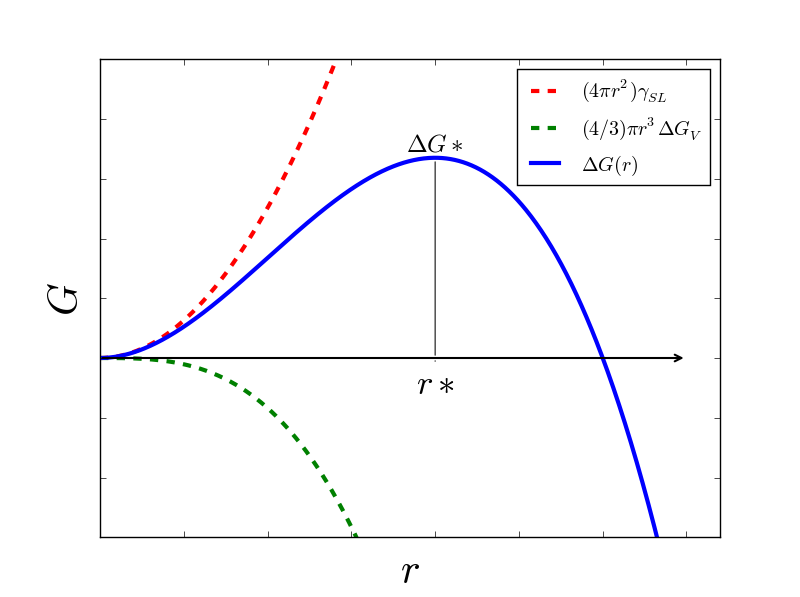
\includegraphics[width=\textwidth]{nucleation_free_energy.png}
		\caption{}
		\label{fig:GibbsNucleation}
	\end{subfigure}
	%Image 2
	\begin{subfigure}[htbp]{0.49\textwidth}
		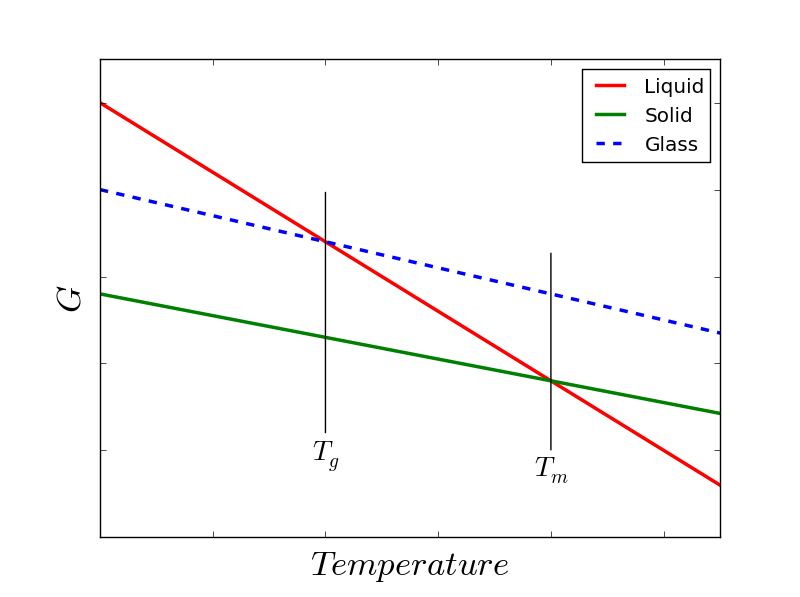
\includegraphics[width=\textwidth]{gibbs_free_energy.png}
		\caption{}
		\label{fig:FreeEnergy}
	\end{subfigure}
	\caption{(a) Homogeneous nuclei within the liquid must reach the \gls{r*} of the \gls{G*} to initiate crystalline growth. (b) Thermodynamically stable materials are always at the lowest \gls{G} state, but can exist in unstable higher free energy states if there is no driving force for the energy reduction.}%global caption
	\label{fig:Gibbs}
\end{figure}
	\todo{Note: Weakly bonded structures have greater free energy slopes due to the large Cp/T dT value
		Assume typical glass bonding Ionic
		Assume typical solid bonding Covalent
		Covalent > Ionic bond strength.
		Thus solid slope < glass
		Glass Tg changes because H and Cp is dependent on cooling rate (i.e. its free energy line is not rigidly defined).}

When a liquid is cooled below its \gls{Tm} without solidifying it is termed a \gls{scl}. Amorphous solids, or glasses, are formed from \gls{scl} by cooling at rates sufficient to suppress the nucleation process entirely. As the \gls{scl} is cooled its \gls{n} increases while its \gls{H} and \gls{V} decrease linearly with temperature at the same rate as the liquid state. As the \gls{n} approaches about $10^{12}$ $Pa*s$ the time scale for molecular rearrangement of the \gls{scl} becomes significantly longer than experimental observation and the \gls{scl} is for all practical purposes 'frozen' as a glass \cite{Ediger1996, Ishii2014}. This transition occurs at the \gls{Tg} and is characterised by a decrease in the rate of change of \gls{H} and \gls{V} with temperature. Note this transition is not a phase change but instead a kinetic event, meaning the material is not technically thermodynamically or kinetically stable, but is treated as stable since the glass does not possess the required kinetic energy to transform into a more stable structure \cite{Ediger1996, Ishii2014}. Being a kinetic event, this means glass' \gls{Tg}, \gls{H}, and \gls{V} are depend on the cooling rate, with faster cooling rates generally producing glasses with higher \gls{Tg}, \gls{H}, and \gls{V} (i.e. quickly cooled glasses have higher services temperatures and reduced density compared to slowly cooled glasses), see Figure \ref{fig:GlassCooling}. \todo{Glass is metastable structure with greater free energy than the crystal state (Ishii, 2014)
	
	Structure does not possess the required kinetic energy to transform into the equilibrium state
	
	Gibbs Free Energy - Lower free energy means a process is more spontaneous. Therefore by thermos crystal is more
	stable than glass.}

%single image
\begin{figure}[htbp]
	\centering
	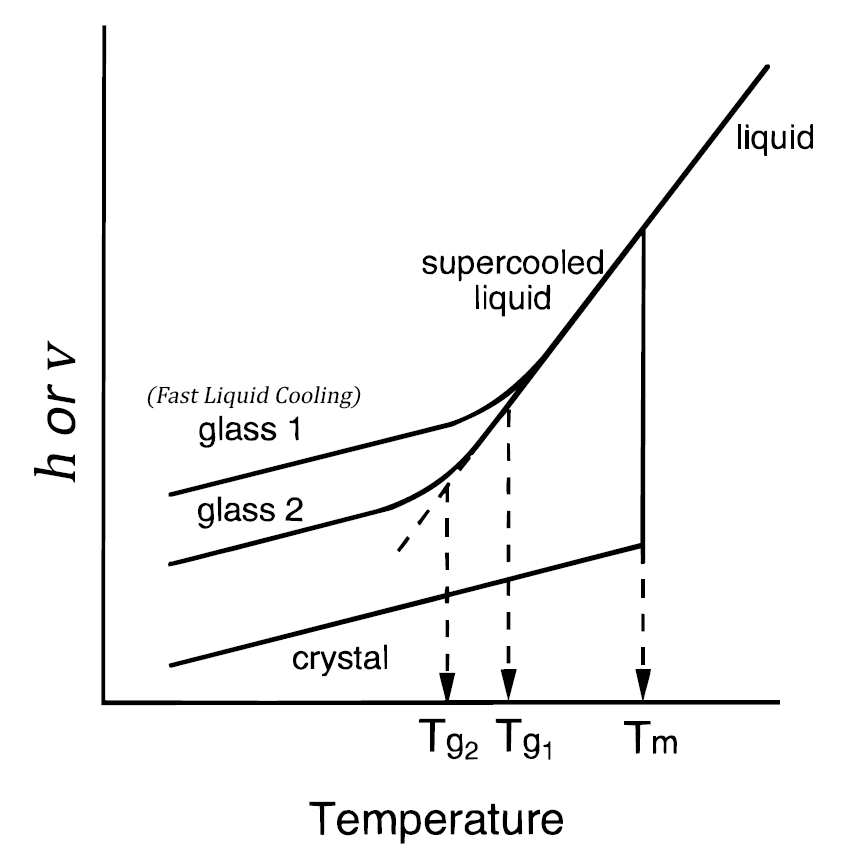
\includegraphics[width=0.75\textwidth]{Glass_Cooling_Graph.png}
	\caption[Schematic of \gls{h} or \gls{v} as a function of temperature for a material that exhibits both glass and crystalline solid states. Note 'glass 1' has a greater \acrshort{Tg} and accordingly greater \gls{h} \& \gls{v} than 'glass 2.' This higher temperature stability is the result of 'glass 1' being cooled more quickly than 'glass 2.']{Schematic of \gls{h} or \gls{v} as a function of temperature for a material that exhibits both glass and crystalline solid states. Note 'glass 1' has a greater \acrshort{Tg} and accordingly greater \gls{h} \& \gls{v} than 'glass 2.' This higher temperature stability is the result of 'glass 1' being cooled more quickly than 'glass 2.' Adapted from \cite{Ediger1996}.}
	\label{fig:GlassCooling}
\end{figure}

As the production demonstrates \glspl{mg} have a similar amorphous atomic structure to liquid metals. This explains \glspl{mg}' relative low density as their atoms are essentially still arranged in a spacious liquid-like configuration (see Figure \ref{fig:GlassCooling}). This liquid-like structure enables \glspl{mg} to excide traditional alloys' solubility limits as the lack of \gls{lro} helps prevents the formation of intermetallic compounds. \glspl{mg} lack of significant plastic deformation is due to the atoms not possessing the required kinetic energy for molecular rearrangement. Hence the atoms are not able to 'slide' past one another to deform as in the molten liquid state.

\subsubsection{Glass Forming Ability (GFA) and Bulk Metallic Glasses (BMGs)}
The ease at which a material is able to form a glass is termed its \gls{gfa}. The \gls{gfa} is also closely tied to a glass's stability with high \glspl{gfa} generally indicating high thermal stability \cite{Aji2013}. Molecular glasses possess sufficiently high \glspl{gfa} and thermal stability that the material has been produced since ancient times, and polymers' \glspl{gfa} are often high enough they can form glass even with slow cooling rates. In contrast metals have such low \glspl{gfa} their amorphous glass state was only discovered in 1960 by Klement, et al. \cite{Klement1960}. \hl{This low GFA results from metals' high atomic mobility, which allows for mgs' fast structural relaxation and recrystallization at elevated temperatures} \cite{Aji2013}. \todo{Maybe more this down to the processing section.}

Much of the work on \glspl{mg} has been to improve their \glspl{gfa} in order to decrease their \gls{Rc}, the rate of quench required to avoid nucleation into the crystalline state \cite{Inoue2000}. From these works it has been discovered alloys with their \gls{Tg} near their \gls{Tm} have higher \glspl{gfa} \cite{Inoue2000, Trexler2010, Turnbull1969}. Meaning the \gls{gfa} of an alloy increases with its \gls{Trg}, given by \gls{Trg} $= T_{g}/T_{m}$ \cite{Inoue2000, Trexler2010, Turnbull1969}. 

From these findings Inoue \cite{Inoue2000} has formulised three rules for high \gls{gfa} systems;

%Bullet List
\begin{itemize}
	\item Multi-component systems of three or more alloy constituents;
	\item Significant difference of above 12\% in atomic size ratios of the three main constituents; and
	\item Negative heats of mixing among the three main constituents (i.e. exothermic reaction). \todo{exothermal = rejects heat!}
\end{itemize}

Alloys that follow these rules display deep eutectics with low \gls{Tm}, sluggish crystallisation kinetics, and accordingly a high $T_{g}/T_{m}$ \cite{Inoue2000, Schroers2010}. The application of these rules has helped to lower \gls{Rc} sufficiently to allow the produce of three-dimensional amorphous alloys with their smallest dimension being at least 1mm, formally referred to as \gls{bmg} formers. These \glspl{bmg} are superior to \glspl{mg} as they possess sufficiently high \glspl{gfa} to allow for these greater dimensions and accordantly display improved thermal stability. As such alloys of \gls{bmg} composition are of the most interests regardless of a sample's desired dimensions, and all alloy compositions henceforth in these works shall be \glspl{bmg} unless otherwise noted. 

%single image
\begin{figure}[htb]
	\centering
	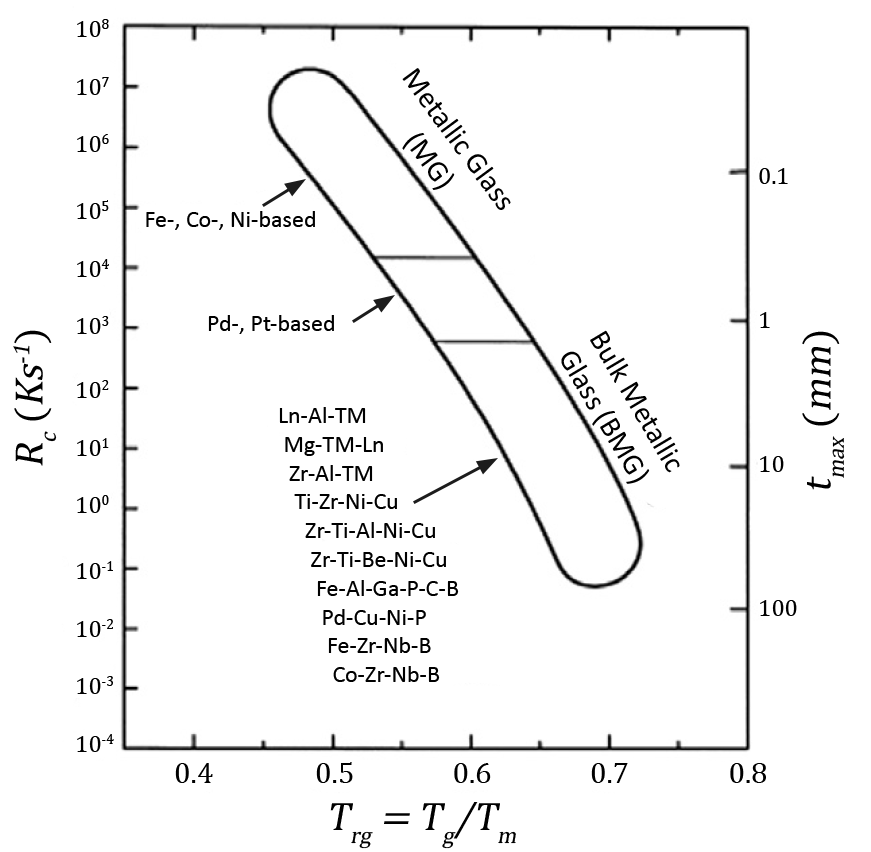
\includegraphics[width=0.75\textwidth]{BMG_Tg_on_Tm_01.png}
	\caption[Schematic of \acrfull{Rc} and \acrfull{tmax} as a function of reduced glass transition temperature (\acrshort{Trg} $= T_{g}/T_{m}$) for a number of glass forming systems. Note the \acrshort{Rc} and \acrshort{tmax} improve with increasing $T_{g}/T_{m}$.]{Schematic of \acrfull{Rc} and \acrfull{tmax} as a function of reduced glass transition temperature (\acrshort{Trg} $= T_{g}/T_{m}$) for a number of glass forming systems. Note the \acrshort{Rc} and \acrshort{tmax} improve with increasing $T_{g}/T_{m}$. Adapted from \cite{Trexler2010}.}
	\label{fig:BMGRc}
\end{figure}

The improvements in \gls{Rc} for amorphous alloy compositions is shown in Figure \ref{fig:BMGRc}, with the defining moment of \gls{bmg} development being denoted by the \gls{tmax} reaching the 1mm mark. Note the \gls{Rc} and \gls{tmax} improve with increasing $T_{g}/T_{m}$, signifying alloys' with larger $T_{g}/T_{m}$ ratios possess higher \glspl{gfa}. 

\subsubsection{BMG Production Methods}
As mentioned, the production of \glspl{bmg} requires the alloys be rapidly quenched at a rate equal or better than their \gls{Rc} in order to avoid crystallisation. For bulk samples these cooling rates are achieved by solidifying the liquid \gls{bmg} alloys onto copper heat sinks capable of extracting heat at the high rates required. The four standard production methods are: \todo{Diamond extracts heat several times faster than Cu. Could industrial diamond be used in BMG production?}

%Bullet List
\begin{itemize}
	\item Gravity Casting: Molten metal is poured under an air \todo{Natural or air atmosphere?} atmosphere into a copper mould to solidify;
	\item Injection Casting: Molten metal under an inert atmosphere is forced by pressure into a copper mould to solidify;
	\item Melt Spinning: Molten metal is solidified onto a water cooled copper wheel, producing ribbons of material; and
	\item Strip Casting: Molten metal is extruded between two water cooled copper rollers, producing continuous plate. 
\end{itemize}

These methods yield cooling rate sufficient for production of simple geometry \glspl{bmg}, but do not allow for complex shapes. Furthermore secondary processing of \glspl{bmg} by methods like machining are often impractical do to the materials' brittleness, low thermal conductivity, and the risk of recrystallization by the processing heat additions. Instead more complex shapes are accomplished by secondary processing conducted above the \glspl{bmg}' \gls{Tg}. 

\subsubsection{BMG Secondary Processing}
A unique property of amorphous metals are once formed they can be heated above their \gls{Tg} into the \gls{scl} temperature range without crystallising for an appreciable amount of time. This is possible because \glspl{bmg} process sufficient thermal stability above their \gls{Tg} to maintain their amorphous structure, i.e. the kinetics for crystallisation are slow \cite{Schroers2010}. At these elevated temperatures \glspl{bmg} display dramatic softening and superplastically as their \gls{n} reduces to its \gls{scl} values, enabling the constituent atoms to flow more freely past each other. 

The introduction of this temporary plastic deformation mechanism allows \glspl{bmg} to be post-processed by \gls{tpf} techniques, similar to thermoplastic polymers. Once the elevated temperature processing is complete the newly formed \gls{bmg} components can be slowly cooled below their \gls{Tg} to the glassy state without initiating crystallisation. This slow cooling helps to eliminate residual internal stresses and allows for high dimensional accuracy in complex \gls{bmg} components \cite{Schroers2010}. Note this processing is unique to \gls{bmg} systems as the more rigid and limited plastic deformation mechanisms of conventional crystalline metallic systems do not support the high deformations of \gls{tpf}.

%single image
\begin{figure}[htb]
	\centering
	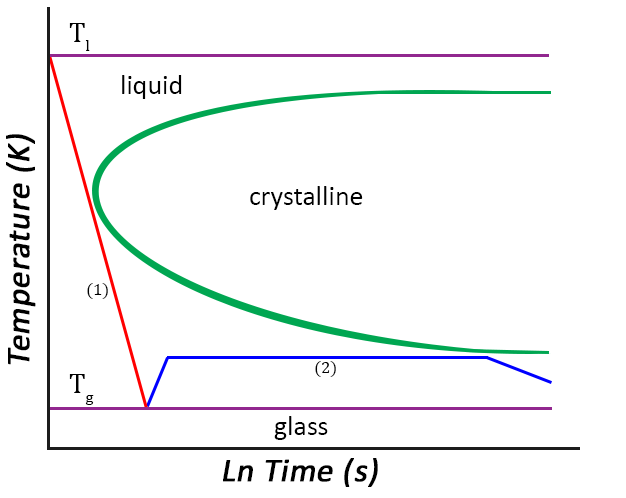
\includegraphics[width=0.75\textwidth]{ProcessingofBMGs_NewDraw.png}
	\caption[Schematic \acrshort{ttt} diagram where line (1) indicates the slowest cooling rate possible to avoid crystallisation and achieve the metallic glass state, and line (2) an elevated temperature processing window above \acrshort{Tg} where metallic glass displays excessive plastic deformation.]{Schematic \acrshort{ttt} diagram where line (1) indicates the slowest cooling rate possible to avoid crystallisation and achieve the metallic glass state, and line (2) an elevated temperature processing window above \acrshort{Tg} where metallic glass displays excessive plastic deformation. Adapted from \cite{Schroers2010}.}
	\label{fig:BMGTTT}
\end{figure}

Figure \ref{fig:BMGTTT} shows a \gls{ttt} diagram for a generic \gls{bmg}. Line (1) of this image shows the minimum \gls{Rc} quench required to completely avoid crystallisation nucleation when forming the \gls{bmg}. Line (2) then displays an elevated temperature processing window available for post-processing of the formed \gls{bmg}. Note with line (2) the processing window stays below the crystallisation zone and displays a gradual cooling once the post processing is complete.

These methods are well suited to the production of \gls{bmg} substrates, but are unsuitable to forming \gls{tfmg}. The \glspl{tfmg} of primary interest for these works must be quenched from the vapour state onto a substrates by deposition techniques.

\section{Thin Films}
\subsection{Thin Film Properties}
Thin films are coatings of less than a nanometre to several micrometres in thickness applied to a substrate with the express purpose of modifying the substrate properties. The application of \glspl{tfmg} to substrates has been shown to have wide spreading effects on properties such as hardness \cite{Chu2012}, \todo{Hardness is tired to wear residence in a few source. Can probably add in those sources.} wear residence \cite{Liu2009, Prakash2005}, fatigue properties \cite{Chiang2006, Chu2011}, corrosion residence \cite{Chu2009}, and surface finish \cite{Liu2009, Chiang2006, Chu2011, Tsai2012}. Chu, et al. \cite{Chu2012} have even demonstrated \glspl{tfmg} can significantly increase \gls{bmg} substrates' bending ductility via modifying the shear band distribution. This ability to dramatically improving substrate properties, and for the films to often display enhanced properties even from equivalent macro \glspl{bmg} makes \glspl{tfmg} an intriguing method for the enhancement of biomaterials.

%single image
\begin{figure}[htbp]
	\centering
	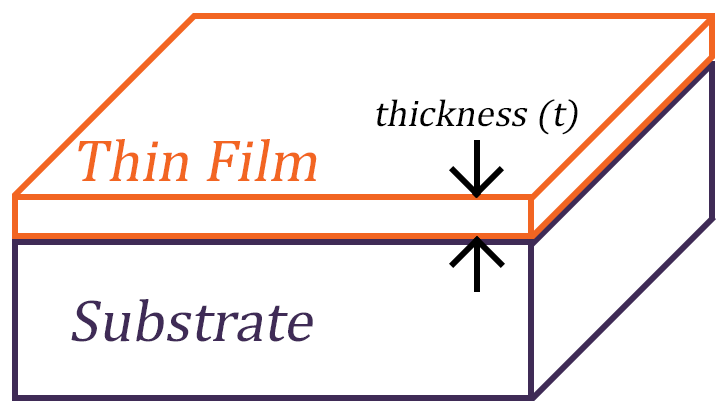
\includegraphics[width=0.50\textwidth]{ThinFilm.png}
	\caption[Schematic of a thin film applied to a substrate to modify its properties. Typical film thickness ($t$) ranges are from a few $nm$ to several $\mu m$ depending on application.]{Schematic of a thin film applied to a substrate to modify its properties. Typical film thickness ($t$) ranges are from a few $nm$ to several $\mu m$ depending on application.}
	\label{fig:ThinFilm}
\end{figure}

\subsection{Production by Deposition}
\Gls{tfmg} coatings are readily produced by \gls{vd} processes such as the \gls{pvd} processes of \gls{pld} and sputtering. These processes produce thin films by condensing vaporised material onto a solid substrate under low vacuum. \todo{The cooling rate achieved are estimated to be as much as 100K within the rotational relaxation time of the material (molecules)! (i.e. fractions of a second!) (Ishii, 2014)}

The \gls{vd} manufacturing route has a significant advantage over traditional \gls{bmg} liquid casting methods in that the composition window is much wider. The vaporised atoms are at much higher vapour pressure than the solid substrate and on impact their kinetic energy is rapidly dissipated into the substrate \cite{Ishii2014}. This greater distance from equilibrium provides a much greater rapid quench for this vapour-to-solid state process than the liquid-to-solid state utilised in \gls{bmg} casting processes \cite{Chu2012b}. 

\subsection{Pulsed Laser Deposition (PLD)}
\Acrfull{pld} produces films primarily by a thermal process under \gls{uhv}. In the process a 'target,' typically rotating, of the desired film material is irradiated and locally vaporised by a 45\degree inclined laser photon pulses. This results in vaporised atoms being ejected from the target as a primarily perpendicular plasma plume, which is directed toward the substrate. Over the course of thousands of repetitions the resulting build-up of atoms produces a thin film (Figure \ref{fig:PLD}). \todo{Note in PLD, the Target atoms are the plasma. (Different from Sputtering). Therefore electrons must re-bond once atoms are deposited onto substrate.}

%single image
\begin{figure}[htbp]
	\centering
	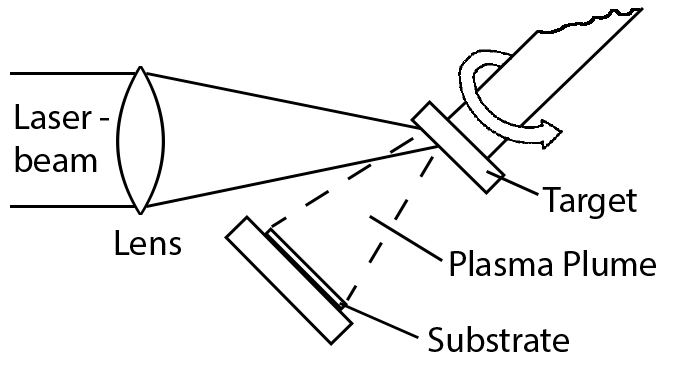
\includegraphics[width=0.75\textwidth]{PLD.png}
	\caption[Schematic of a typical \acrshort{pld} setup showing the incoming laser beam inclined at an approximate 45\degree angle to the target, and the rotating target and substrate parallel to each other.]{Schematic of a typical \acrshort{pld} setup showing the incoming laser beam inclined at an approximate 45\degree angle to the target, and the rotating target and substrate parallel to each other. Adapted from \cite{Krebs1993}.}
	\label{fig:PLD}
\end{figure}

\subsubsection{PLD Advantages}
The key advantage of \gls{pld} is it is able to deposit films of the same stoichiometric ratio, or composition, as its targets \cite{Dijkkamp1987, Heitz1990}. This is significant as it means deposited films have the same elemental composition as their target material. As the compositions of \glspl{bmg} are generally carefully chosen this is practically useful as it streamlines achieving the desired \gls{tfmg} compositions. 

\subsubsection{PLD Challenges}
The work of Cao \cite{Cao2013} has identified potential problems in the \gls{pld} deposition of \glspl{tfmg} with achieving quality surface finishes and recrystallization of amorphous targets. It appears the deposition times of the \gls{pld} allow for sufficient heat to be applied to amorphous targets to cause partial crystallisation (Figure \ref{fig:ReCryTarget}), while still achieving amorphous \glspl{tfmg} depositions onto the examined crystalline zirconium substrates. As \gls{pld} is by definition a thermal deposition process preventing this heat from entering the targets could be difficult. And it remains to be examined if this excess heat could affect the substrates; i.e. recrystallization of amorphous substrates, \gls{pcl} scaffolds strength, thermal breakdown of the scaffold payloads, etc. Naturally this heat is a moot point when examining standalone \glspl{tfmg} as these specimens are separated from their substrate after deposition. 

%single image
\begin{figure}[htbp]
	\centering
	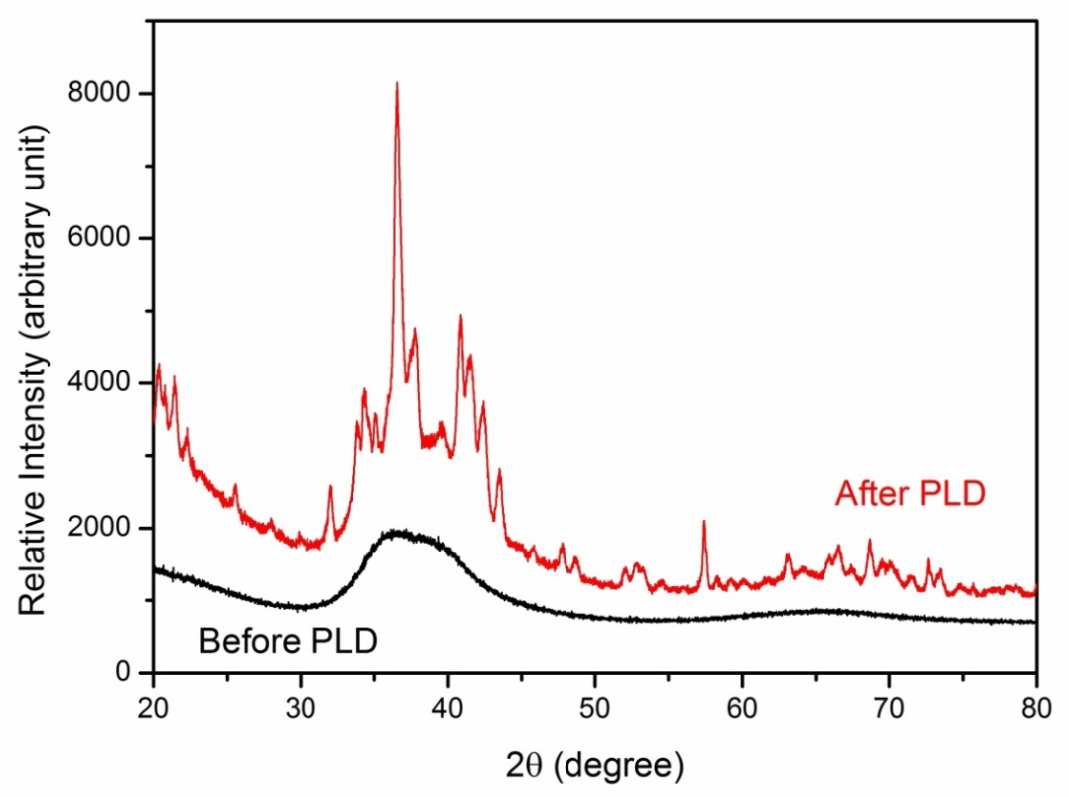
\includegraphics[width=0.75\textwidth]{CaoThesis_XRDTarget.png}
	\caption[Amorphous target \acrshort{xrd} scan before (black curve) and after (red curve) \acrshort{pld} showing the shift from characteristic amorphous structure to crystalline.]{Amorphous target \acrshort{xrd} scan before (black curve) and after (red curve) \acrshort{pld} showing the shift from characteristic amorphous structure to crystalline. Reproduced from \cite{Cao2013}.}
	\label{fig:ReCryTarget}
\end{figure}

\Gls{pld} \gls{tfmg} surface finish droplet defects have been observed by Krebs and Bremert \cite{Krebs1993} and later Cao \cite{Cao2013}. It is suggested these defects are intrinsic to the setup configuration and cannot be eliminated by refining the \gls{pld} parameters. It is further proposed it may be possible to achieve higher quality surface finishes with setup modifications such as the addition of a mechanical velocity filter to remove slower, droplet depositing prone particles from the plasma plume. Another option is dual-beam ablation geometry which utilised two colliding laser ablation to redirect the coating to a substrate outside the direct path of both plumes, preventing heavier droplet depositing prone particles from reaching the substrate. Note both of these methodologies reduce the deposition rate and it remains to be seen if these changes are practical to implicate at \acrshort{unsw}.

\subsection{Sputtering Deposition}
Sputtering deposition is similar to \gls{pld} in that it also coats a substrate with material transferred from a target under vacuum. The essential difference is sputtering utilises the momentum of colliding plasma cations, instead of lasers, to accomplish the transfer. \todo{The voltage potential between the substrate and target supplies excess electrons to the negative target. The electrons are attracted to the positive substrate but collide with Ar atoms on their journey. This cause Ar to lose an electron and to become a plasma (Ar+ + e-). Ar+ collide with the target, and releases M atoms from the target. (Note e- has too little momentum to eject atoms from substrate).
Thus the M atoms are neutral charge (not plasma) because they are not being impacted by electrons in the field.}

\subsubsection{Direct Current (DC) Sputtering} 
\Gls{dc} sputtering applies a high-voltage to create a circuit between the target and substrate, forming a negative (cathode) and positive (anode) electrode respectively. The high-voltage electric field generated within the chamber ionises the low pressure inert working gas, generally Argon, into a plasma, with its positivity charged cations being attracted to the negative target. When the charged cations collide with the target the moment exchange dislodges atoms from the target's surface and expelled them in all directions. A portion of these free, non-ionised target atoms are ejected toward the substrate surface and on impact are deposited as the thin film (Figure \ref{fig:Sputter_Schematic}). \todo{Because the Target and Substrate gap is not insulted, like in a capacitor, current can flow between the two. Providing the electrons as detailed above.}

%code to put 2 images side by side in a figure
\begin{figure}[bp]
	\centering
	%Image 1
	\begin{subfigure}[htbp]{0.75\textwidth}
		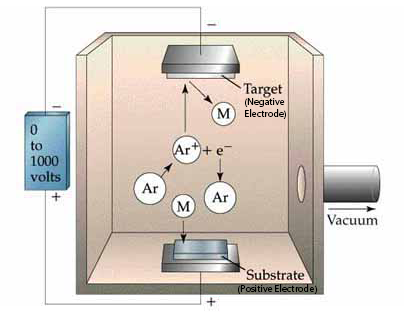
\includegraphics[width=\textwidth]{Sputtering_02.png}
		\caption{}
		\label{fig:Sputter_Schematic}
	\end{subfigure}
	%Image 2
	\begin{subfigure}[htbp]{0.75\textwidth}
		\includegraphics[width=\textwidth]{Field_Sputtering.png}
		\caption{}
		\label{fig:Field_Sputtering}
	\end{subfigure}
	\caption[(a) Schematic of a typical \acrshort{dc} sputtering setup with an Ar working gas. The high-voltage field generates and propels Ar+ cations toward the negative target of material 'M.' Dislodged neutral 'M' atoms are hurled in all directions with some being deposited onto the positive substrate. (b) Schematic of magnetron sputtering deposition showing magnetic field line's effect on the working Ar plasma. Note target 'M' atoms remain neutrally charged.]{(a) Schematic of a typical \acrshort{dc} sputtering setup with an Ar working gas. The high-voltage field generates and propels Ar+ cations toward the negative target of material 'M.' Dislodged neutral 'M' atoms are hurled in all directions with some being deposited onto the positive substrate. (b) Schematic of magnetron sputtering deposition showing magnetic field line's effect on the working Ar plasma. Note target 'M' atoms remain neutrally charged. (a) Modified from \cite{Brown2014}.}%global caption
	\label{fig:Sputter}
\end{figure}

The key advantage of \gls{dc} sputtering when working with amorphous materials is it able to accommodate low working temperatures as the momentum mechanism avoids adding unnecessary heat to the targets and substrates. Additionally, while Ar is a convenient working gas, greater deposition efficiency can be achieved when depositing lighter or heavier elements by working with lighter or heavier gases, respectively. These characteristics help make it possible to deposit most \glspl{bmg} by \gls{dc} sputtering. 

\subsubsection{Magnetron Sputtering}
Magnetron sputtering is a variant of \gls{dc} sputtering which improves ionisation efficiency by applying a magnetic field to trap the charged plasma cations near the target surface. This trap also increases the total volume of plasma cations by trapped free electrons colliding with neutral working gas atoms and ionising them. The extra target collisions from these two effects increases the deposition rate even at lower working pressures . For these reasons this variant is prevalent in most recent studies and all further mention of sputtering shall be magnetron sputtering, unless otherwise noted. \todo{Advantage of Sputtering is higher pressure than PLD. Maybe a better way to word this.}

\subsubsection{Sputtering Advantages}
While the momentum exchange mechanism of sputtering allows for the use of amorphous targets when depositing \gls{tfmg} (i.e. excess heat is not added to the system) it has been found the use of crystalline targets results in no appreciable difference in the quality, composition, and structure of the substrate coating \todo{Find more sources to back this up. - Jake got closer to this conclusion, but did not quite make it.} \cite{Liu2012}. Instead, as shown by Liu, et al. \cite{Liu2012} work on the \ZrCuNiAl~ system, the coating quality and production of \gls{tfmg} is primarily controlled by the Ar pressure and sputtering power parameters. This has implications for practical application production runs as crystalline targets are easier, quicker and cheaper to produce than amorphous ones. 

When depositing \glspl{tfmg} it has been observed the deposition rate is proportional to the sputtering power, and that higher rates result in smoother film surfaces \cite{Cao2013, Liu2012}. Additionally, Liu, et al. \cite{Liu2012} have found a dynamic smoothing effect occurs making it possible to produce atomically flat \glspl{tfmg} with low Ar pressure and high sputtering power. 

\subsubsection{Sputtering Challenges}
One of the core challenges with single target magnetron sputtering is it can be difficult to achieve the same stoichiometric ratio as the target alloy when depositing multi-component \glspl{tfmg} \cite{Cao2013, Liu2012, Kondoh2008}. This occurs because lighter elements dislodged from the target more easily when subjected to ion bombardment, resulting in different sputtering yields for each element of multicomponent targets. It is possible to remedy the situation through the use of multiple pure element targets, called combination deposition \cite{Deng2007, Qin2009, Apreutesei2014}, but as shown by Liu, et al. \cite{Liu2012} this method may not be necessary. Liu, et al. \cite{Liu2012} found it is possible to deposit \glspl{tfmg} with the same composition as their \ZrCuNiAl~ target by refining the Ar pressure and sputtering power parameters. As this solution requires only a single target and no modifications to the sputtering set up it seems reasonable to examine it first with the Mg based systems. 

\subsection{Preferred PVD Methods}
Thus despite sputtering having more difficulties than \gls{pld} when refining the stoichiometric ratios for deposition, it is has been concluded it the superior deposition method. This is primarily because of its significant advantages; non-thermal process, higher operating pressures, faster deposition rates, and better surface finishes. For these reason sputtering shall be the preferred method for \gls{tfmg} deposition in these works. 

\section{Ultrastable Glass (USG)} \todo{SMG corrosion has not been studied!!!}
\subsection{Introduction}
\Glspl{usg} are \gls{vd} produced amorphous films in a low energy state generally characterised by high thermodynamic and kinetic stabilities, low entropy, high density, high elastic modulus, and always by an \gls{dTg}. The \gls{dTg} phenomenon is their defining characteristic as it indicates the high kinetic stability due to the higher temperatures required to dislodge their atoms from the glassy configuration \cite{Swallen2007, Dawson2011}. This naturally extends to give \glspl{usg} higher service temperatures, and hence higher softening temperatures relative to their ordinary glass counterparts. \todo{Cut high density/modulus so next section is less redundant?}

\subsection{USG General Properties and Development}
The defining characteristic of \glspl{usg} are the \gls{dTg} and accordingly their high kinetic stability. They also generally are at a low-thermodynamic-energy state exhibited by low enthalpy, have a high density, and possess a high elastic modulus. These effects can be significant as demonstrated by Aji, et al. \cite{Aji2013} whom produced materials with 30\% gains in elastic modulus and hardness. 

To date the only developed \glspl{usg} are organic, molecular and polymer glasses, with only a handful of attempts being made to produce \glspl{smg} \cite{Aji2013, Yu2013, Wang2014}. Part of the reason for this is it unclear if the more simple atomic structures of metallic alloys, relativity to molecular and polymer glasses, are suitable to form \glspl{usg} \cite{Yu2013}. Nevertheless the work of Yu, et al. \cite{Yu2013}, Aji, et al. \cite{Aji2013}, and Wang, et al. \cite{Wang2014} on Zr and Au alloy systems have established the initial understandings of what appear to be \glspl{smg}, though it remains to be seen how the established trends will extend to other metallic systems. 

\subsection{USG Production}
Production of \glspl{usg} is by low rate, low pressure \gls{vd} techniques onto substrates at elevated temperature \cite{Ishii2014, Aji2013, Yu2013, Wang2014, Nakayama2013}. This method allows sufficient time for the molecular relaxation kinetics of glasses to rearrange into highly efficient packing structures \cite{Aji2013, Swallen2007, Wang2014}. This initial work on \glspl{usg} shows the more complicated the deposition material's atomic structure the higher the \gls{Tsub} must be \cite{Yu2013}. Accordingly the ideal \gls{Tsub} for a \gls{smg} is 0.7 $-$ 0.8 \gls{Tg}, while it is 0.75 $-$ 0.85 \gls{Tg} for the more complicated molecular glasses \cite{Swallen2007, Dawson2011, Yu2013, Dawson2010, Kearns2008}. 
 
Yu, et al. \cite{Yu2013} has noted that while more complicated atomic structures require higher temperatures to arrange into \gls{usg} configurations no definite mechanism has been identified for why the ideal ranges are well below the \glspl{usg}' \gls{Tg}. Theoretically higher temperatures should allow for more efficient rearrangement of atoms, but this does not happen due to unidentified limiting factors. Ishii and Nakayama \cite{Ishii2014} suggest increased diffusion and quicker relaxation times at the surface may be responsible while Yu, et al. \cite{Yu2013} extends, suggesting the quicker relaxation times lead to a lower \gls{Tg} at the \gls{usg} surface. This implies the surface atoms behave as a \gls{scl}, meaning the atoms have essentially been quenched from the liquid state instead of being directly deposited from the vapour state \cite{Yu2013}. It is anticipated the simple atomic structure of \glspl{smg} could serve as model material in the study of these glass thermodynamics and kinetics phenomena \cite{Yu2013, Wang2014}. 

%single image
\begin{figure}[htb]
	\centering
	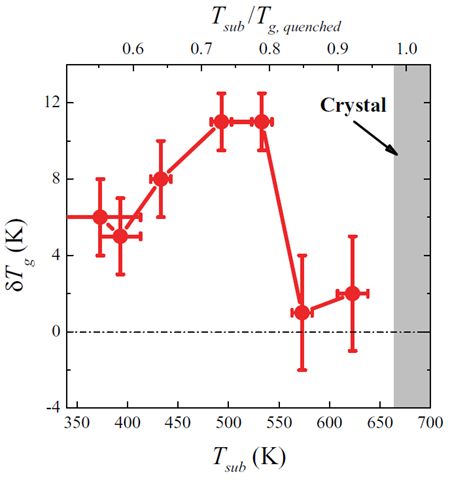
\includegraphics[width=0.75\textwidth]{Tsub_Yu_SMG.png}
	\caption[Relationship between \acrshort{Tsub} and \acrshort{dTg} for the Yu, et al. \acrshort{smg}. Data clearly shows deposition at \acrshort{Tsub} outside of the ideal temperature range results in poor \acrshort{usg} \acrshort{dTg} gains.]{Relationship between \acrshort{Tsub} and \acrshort{dTg} for the Yu, et al. \cite{Yu2013} \acrshort{smg}. Data clearly shows deposition at \acrshort{Tsub} outside of the ideal temperature range results in poor \acrshort{usg} \acrshort{dTg} gains. Reproduced from \cite{Yu2013}.}
	\label{fig:YuTsub}
\end{figure}

Non-\gls{vd} production techniques do not allow sufficient rearrangement time to form \glspl{usg} as is demonstrated by organic glass where a reduction in cooling rate by a factor of 10 typically only decreases the \gls{Tg} by 3 $-$ 5 kelvin \cite{Ediger1996, Dawson2011}. \todo{Dawson reference other papers before this, but made the conclusion. Can I site him, or should I go to his source material? Check the “Tg + Tf paper” as it should have first principles reference to this.} The results of the \gls{vd} techniques cannot even be replicated with extensive artificial aging or annealing times below \gls{Tg}. For example Swallen, et al. \cite{Swallen2007} found with organic glass \todo{Organic glasses are carbon based, molecular are Si or other elements.} the ultrastable effects could not be replicated even when annealed below their \gls{Tg} for 6 months, and when working with Kearns, et al. \cite{Kearns2008} went on to show the theoretical annealing time required would be at least 1000 years. Additionally both Aji, et al. \cite{Aji2013} and Wang, et al. \cite{Wang2014} showed annealing \glspl{smg} can completely remove the ultrastable effects, implying any production materials should have their service temperatures and thermal creep carefully evaluated.

\subsection{SMG Characterisation}
Additional insight into the thermodynamic and kinetic stability, general properties, and structure of \glspl{smg} have been identified by a number of characterisation and modelling techniques. 

\subsubsection{Fictive Temperature (\Tf), Kinetic Stability and Enthalpy by Differential Scanning Calorimetry (DSC)}
\Gls{dsc} is an analytical technique that measures the heat flow of an unknown sample. This is done by raising its temperature linearly at the same rate as a reference sample with a known heat capacity. This allows phase changes to be detected in the unknown sample as more or less heat will need to be applied to it to maintain both samples at the same temperature. This can be used to detect melting, crystallising, and other changes like glass transition in a sample.

With amorphous materials the analysis displays an exothermic 'step in the baseline' as the sample reaches its \gls{Tg} because it undergoes a change in its heat capacity. Upon further heating many amorphous materials spontaneously rearrange themselves into an ordered crystalline structure. This \gls{Tx} \todo{Crystallisation is exothermic because the LRO has a lower free energy than SRO glass (So the transformation releases energy). Solid to liquid causes an increase in rate of change of free energy, hence it is endothermic.} is recorded as an exothermic peak. With further heating the \gls{Tm} and \gls{Tl} are reached and recorded as endothermic peaks, \todo{Melting of solid to liquid is an endothermic reaction (i.e. heat needs to be supplied to the reaction).} absorbing energy. Note these peaks correspond with Gibb's Free Energy, \todo{Free energy always decreases. Tg to Tx reduces energy as there are kinetics for atoms to move to lowest energy state. Tx to Tm/Tl reduces energy because Liquid free energy line has greater rate of change than solid.} with system restructuring to more ordered lower energy states being exothermic (i.e. glass to crystalline), and disordered lower energy states being endothermic (i.e. crystalline to liquid), see Figure \ref{fig:FreeEnergy}.

Using \gls{dsc} the kinetic stability of glass can be measured by shifts in the \gls{Tonset}, which appear as the first 'step in the baseline' in the \gls{dsc} \gls{cp} trace; identifying the start of the \gls{Tg} region. Shifts in the \gls{Tonset} to higher temperatures identify an increase in heat capacity as the atoms need to absorb more energy to become mobile; indicating the higher kinetic stability with a higher \gls{Tg} \cite{Kearns2008}. The value of the \gls{Tg} is generally taken as the maxima of the derivative of trace with respect to temperature.

A \acrfull{h} curve from the \gls{dsc} trace can be obtained by integrating the original \gls{Cp} trace, with respect to temperature. Using this curve the \gls{Tf} \todo{Find a proper/ full definition of Tf!} can be used to establish the enthalpy of the glass \todo{Tf measures enthalpy. I.e. High Tf means higher enthalpy.} by measuring were the film's enthalpy line interests the extrapolated \gls{scl} enthalpy line of the bulk material (Figure \ref{fig:DSC_IMC_PMMA}) \cite{Kearns2008}. An ordinary glass's enthalpy appears at \gls{Tf} $=$ \gls{Tg} on the trace, whereas an ultrastable glass's is expected to have a lower \gls{Tf} and lower enthalpy at \gls{Tf} $<$ \gls{Tg}. 

%code to put 2 images side by side in a figure
\begin{figure}[bp]
	\centering
	%Image 1
	\begin{subfigure}[htbp]{0.70\textwidth}
		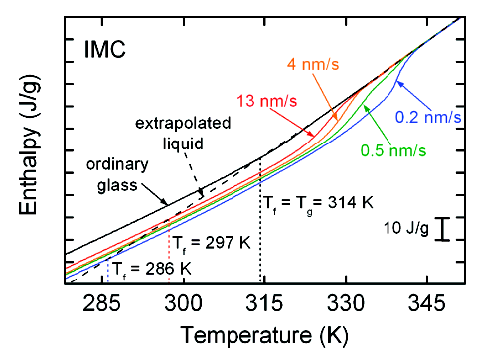
\includegraphics[width=\textwidth]{Kearns_DSC.png}
		\caption{}
		\label{fig:DSC_IMC}
	\end{subfigure}
	%Image 2
	\begin{subfigure}[htbp]{0.70\textwidth}
		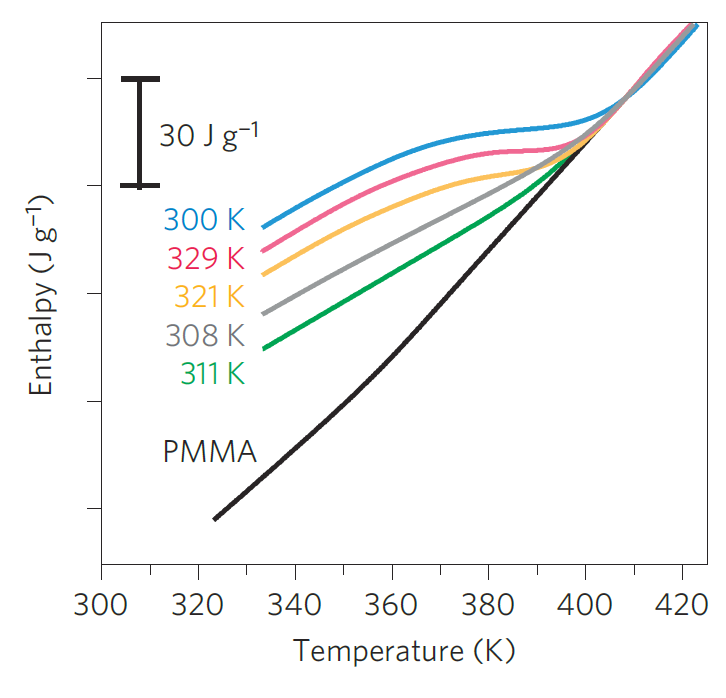
\includegraphics[width=\textwidth]{Guo_DSC.png}
		\caption{}
		\label{fig:DSC_PMMA}
	\end{subfigure}
	\caption[(a) An integrated \acrshort{dsc} trace for the molecular IMC glass system displaying the various values of \acrshort{Tf} obtained when varying the deposition rate (the coloured lines). Note all deposited glasses have a reduced \acrshort{Tf} indicating a reduction in enthalpy compared to ordinary glass. (b) An integrated \acrshort{dsc} trace for the polymer PMMA system showing increased enthalpy with varied substrate temperature.]{(a) An integrated \acrshort{dsc} trace for the molecular IMC glass system displaying the various values of \acrshort{Tf} obtained when varying the deposition rate (the coloured lines). Note all deposited glasses have a reduced \acrshort{Tf} indicating a reduction in enthalpy compared to ordinary glass. (b) An integrated \acrshort{dsc} trace for the polymer PMMA system showing increased enthalpy with varied substrate temperature. Reproduced from \cite{Kearns2008} and \cite{Guo2012} respectively.}%global caption
	\label{fig:DSC_IMC_PMMA}
\end{figure} \todo{Technically fig:DSC IMC (a) may be Organic (Figure of the molecular structure has C-rings).}

Most developed \glspl{usg} and the new \glspl{smg} display reduced enthalpy, as improved stability predicts \cite{Aji2013, Wang2014}. However the work Yu, et al. \cite{Yu2013} and Guo, et al. \cite{Guo2012} on \glspl{smg} and polymer \glspl{usg} respectively have shown exceptions with high enthalpy being coupled with high kinetic stability \gls{dTg}. When this occurs the enthalpy traces of \glspl{usg} are greater than ordinary glass and intersect higher on the \gls{scl} line with \gls{Tf} $>$ \gls{Tg}. This contradiction with Kearns, et al. \cite{Kearns2008} demonstrates that \gls{Tonset} and \gls{Tf} are not coupled together and act independently in \gls{usg} systems. Accordingly both parameters should be examined when studying new \gls{smg} materials. 

\subsubsection{The Theoretical Entropy Limit of Glasses and the Kauzmann Temperature (\Tk)}
Normally a glass is formed when a material's \gls{scl} solidifies on reaching its \gls{Tg}. However if the \gls{scl} could be lowered to the \gls{S} of its crystalline state before solidifying it would achieve the theoretical lowest thermodynamic-energy state possible and its 'ideal' \gls{Tg}, known as the \gls{Tk}, \todo{“Tk is usually determined by extrapolation of supercooling liquid entropy to the temperature where S(liquid) = S(crystal)” (Angell, 2014)} (Figure \ref{fig:TkGraph}) \cite{Swallen2007, Kearns2008}. \todo{Have some other references around this point. Should have a look at them.} This makes \gls{Tk} a useful limit to evaluate the effectiveness of the improvements in thermodynamic stability of \glspl{usg}. 

%single image
\begin{figure}[htbp]
	\centering
	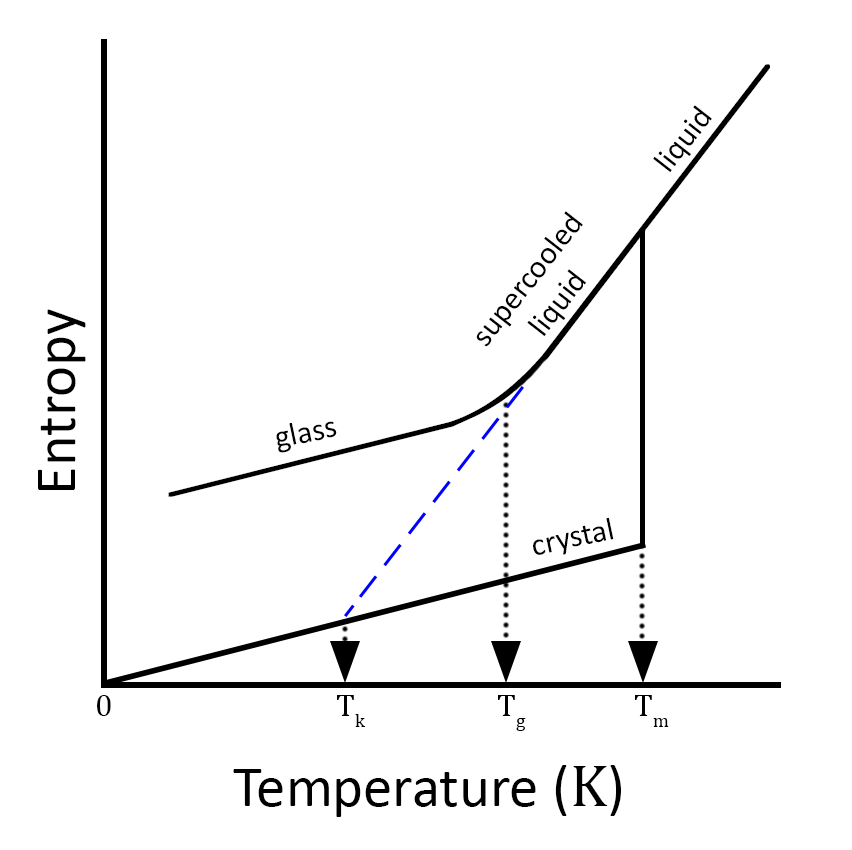
\includegraphics[width=0.75\textwidth]{Tk_Graph_New_Draw.png}
	\caption[Schematic of glass temperature vs entropy in a typical glass forming system. The \acrfull{Tk} represents the \acrfull{Tg} of an ideal glass. The blue line is the extrapolated \acrshort{scl} line and the ideal path.]{Schematic of glass temperature vs entropy in a typical glass forming system. The \acrfull{Tk} represents the \acrfull{Tg} of an ideal glass. The blue line is the extrapolated \acrshort{scl} line and the ideal path. Adapted from \cite{Ediger1996, Kearns2008}.}
	\label{fig:TkGraph}
\end{figure}

Rewriting Swallen, et al. \cite{Swallen2007} and Kearns, et al. \cite{Kearns2008} equation for \gls{ok} to measure between \gls{Tk} and \gls{Tg} the following expression is obtained. 

%numbered display equation
\begin{equation}
\theta_{k} = 1 - \frac{T_{g}-T_{f}}{T_{g}-T_{k}}
\label{equ:EngeryLandscape}
\end{equation}

Equation \ref{equ:EngeryLandscape} follows the extrapolation \gls{scl} line of a glass and calculates an entropy ratio relative to the glass's ideal \gls{Tk} and its \gls{Tg}. From this it is seen an ideal glass with \gls{Tf} $=$ \gls{Tk} results in \gls{ok} $=0.0$, signifying the glass has reached the bottom of the energy landscape \cite{Swallen2007, Kearns2008}. While an ordinary glass with \gls{Tf} $=$ \gls{Tk} results in \gls{ok} $=1.0$, signifying the glass has not moved down the energy landscape (it is 100\% the distance between \gls{Tk} and \gls{Tg}).

Thus for real \glspl{usg} with reduced entropy \todo{Tf was used in enthalpy before Should this be ‘enthalpy’ instead of ‘entropy’?} the \gls{ok} falls between 0.0 and 1.0, while the higher entropy \glspl{smg} of Yu, et al. \cite{Yu2013} would yield \gls{ok} greater than 1.0, indicating they have moving up the energy landscape past the \gls{Tg} datum. For example, a \gls{ok} $=1.25$ would indicate a glass's entropy is 125\% greater than its ideal \gls{Tk} glass.

\subsubsection{Glass Fragility (m)}
The \gls{m} \todo{Angell invented this relationship in old paper. Should use it more as source on m. (Angell, 1995)} of a glass is a measure of its deviation from ideal Arrhenius behaviour; defined as the rate of change of the glass's \acrfull{n} as a function of reduced inverse temperature scaled by the glass transition temperature ($T_{g}/T$).

%numbered display equation
\begin{equation}
m \equiv 
\frac{\partial log_{10} (\eta)}
{\partial (\frac{T_{g}} {T})}
\biggr|_{T=T_{g}}
\label{equ:Fragility}
\end{equation}

The more a glass varies from this ideal Arrhenius behaviour the more 'fragile' it is, and higher its \gls{m} value. Highly fragile glasses, or 'weak' glasses, vary significantly from the ideal Arrhenius behaviour, and generally experience substantial deviations in heat capacity with temperature \cite{Shelby2005, Angell1995}. In contrast low fragility, or 'strong' glasses, have little variation from Arrhenius behaviour and usually experience little change in heat capacity with temperature. Whether a glass is strong or weak typically depends on the atomic structure, with \glspl{bmg} generally characterised as 'strong', polymers as 'weak,' and molecular glasses somewhere in between, see Figure \ref{fig:ShelbyFragPlot}. 

%single image
\begin{figure}[htb]
	\centering
	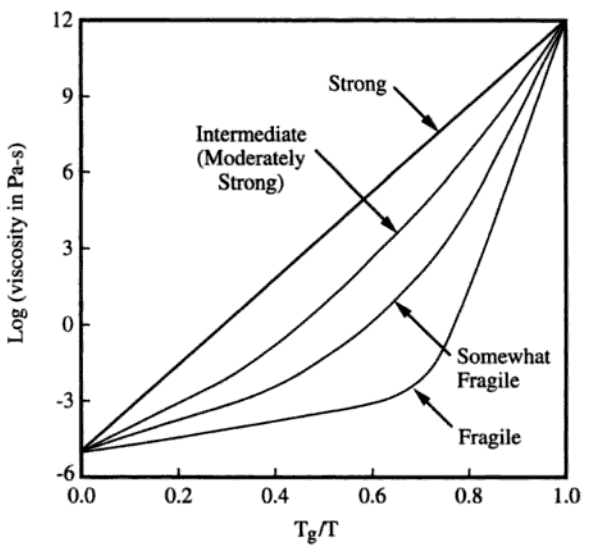
\includegraphics[width=0.75\textwidth]{ShelbyFragilityPlot.png}
	\caption[Viscosity as a function of reduced inverse temperature ($T_{g}/T$) for strong to weak glasses over the flowing range of viscosities. Note the 'ideal' strong glass displays a constant exponential slope over the full temperature range, while weaker glass' slopes very.]{Viscosity as a function of reduced inverse temperature ($T_{g}/T$) for strong to weak glasses over the flowing range of viscosities. Note the 'ideal' strong glass displays a constant exponential slope over the full temperature range, while weaker glass' slopes very. Adapted from \cite{Shelby2005}.}
	\label{fig:ShelbyFragPlot}
\end{figure}

Yu, et al. \cite{Yu2013} found \gls{m} of metallic, molecular, and polymer \glspl{usg} correlate with $\delta T_{g}/T_{g}$, which is surprising given the notable difference in their atomic structures, bonding, and deposition rates (Figure \ref{fig:YuMTgPlot}). From these initial findings it appears greater improvements in \gls{dTg} in relation to the standard \gls{Tg} correlates with more fragile glasses (i.e. high m values supports high \gls{dTg}). Despite Yu, et al. \cite{Yu2013} providing the only \gls{smg} data a review of multiple glass systems by Angell \cite{Angell2014} supports this fragility relationship, suggesting the \gls{dTg} improvements for \glspl{smg} may have a modest limit. 

%single image
\begin{figure}[htb]
	\centering
	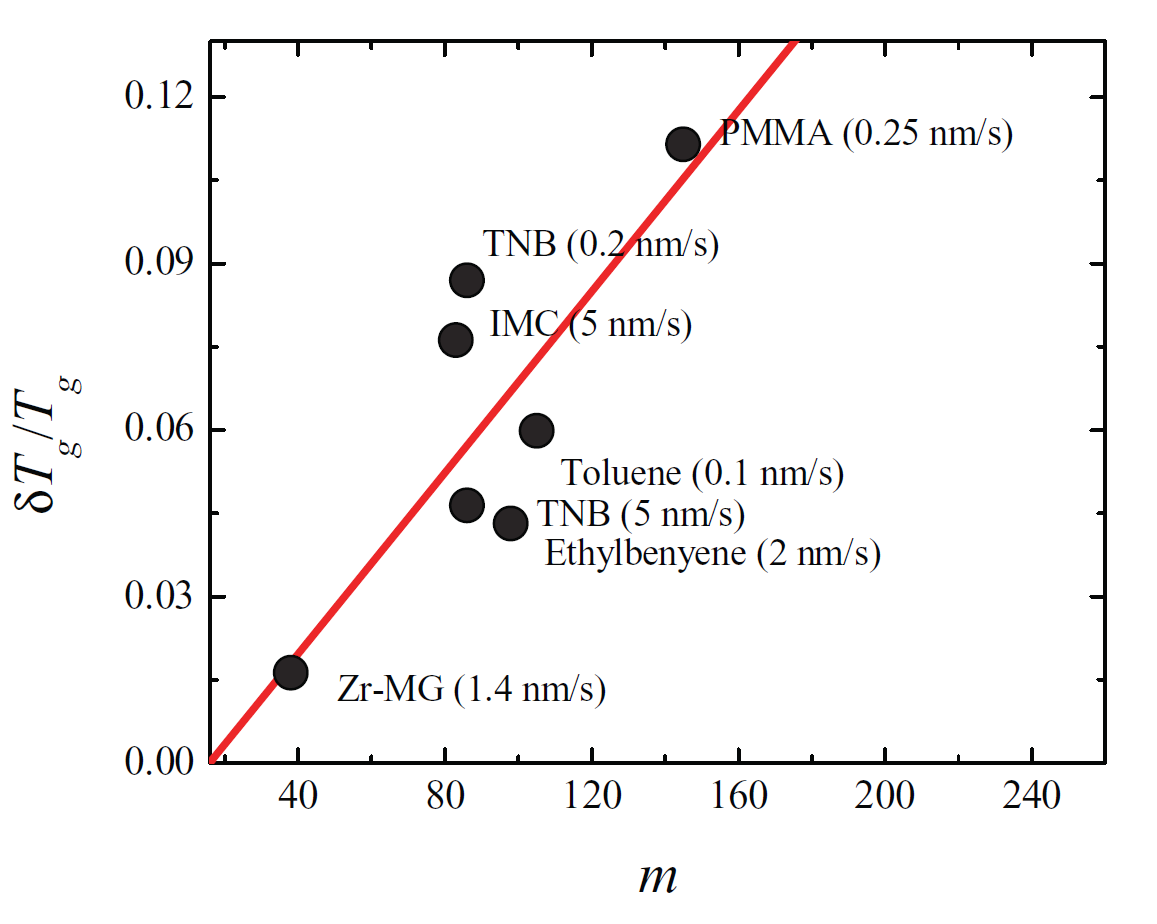
\includegraphics[width=0.75\textwidth]{YuMTg.png}
	\caption[Schematic of the relationship between glass \gls{m} and the enhanced glass transition on glass transition ratio ($\delta T_{g}/T_{g}$) for a selection of metallic, molecular, and polymer \acrshort{usg}s.]{Schematic of the relationship between glass \gls{m} and the enhanced glass transition on glass transition ratio ($\delta T_{g}/T_{g}$) for a selection of metallic, molecular, and polymer \acrshort{usg}s. Reproduced from \cite{Yu2013}.}
	\label{fig:YuMTgPlot}
\end{figure}

\subsubsection{Glass Density (\p)} 
\Gls{usg} are characterised as being denser than their liquid quenched counterparts \cite{Wang2014}. This is somewhat unexpected as traditional glass theory predicts more rapid cooling should produce lower density glass coupled with higher \gls{Tg} (see Figure \ref{fig:GlassCooling}). It appears the process of depositing atoms/molecules layer by layer by \gls{vd} allows glasses to achieve both enhanced density and \gls{Tg}, though Nakayama, et al. \cite{Nakayama2013} point out that while the deposition conditions for dense glass seem to match those of \gls{usg}, it is not yet clear if the two phenomena are the same class of material.

Ishii and Nakayama \cite{Ishii2014} and Nakayama, et al. \cite{Nakayama2013} have found a relationship between deposition temperature and a decrease in molar volume, i.e. increased density, with many molecular glasses. The relationship shows the density of \gls{usg} increase with the \gls{Tsub} up to the \gls{usg} formation temperature limit (see Section 2.3.1) \cite{Ishii2014, Nakayama2013}. Swallen, et al. \cite{Swallen2007} has also observed a very similar relationship between organic glass density and \gls{Tsub}. Dawson, et al. \cite{Dawson2010} suggest the higher temperatures permit the molecules more surface mobility to arrange into more ordered and dense structures, while a low \gls{Tsub} does not provide the required kinetic energy for this efficient rearrangement. This mechanism suggest the \glspl{usg} density can be further increased by reducing the deposition rate as the molecules/atoms have more time to arrange into ordered structures \cite{Dawson2010}.

%code to put 2 images side by side in a figure
\begin{figure}[bp]
	\centering
	%Image 1
	\begin{subfigure}[htbp]{0.75\textwidth}
		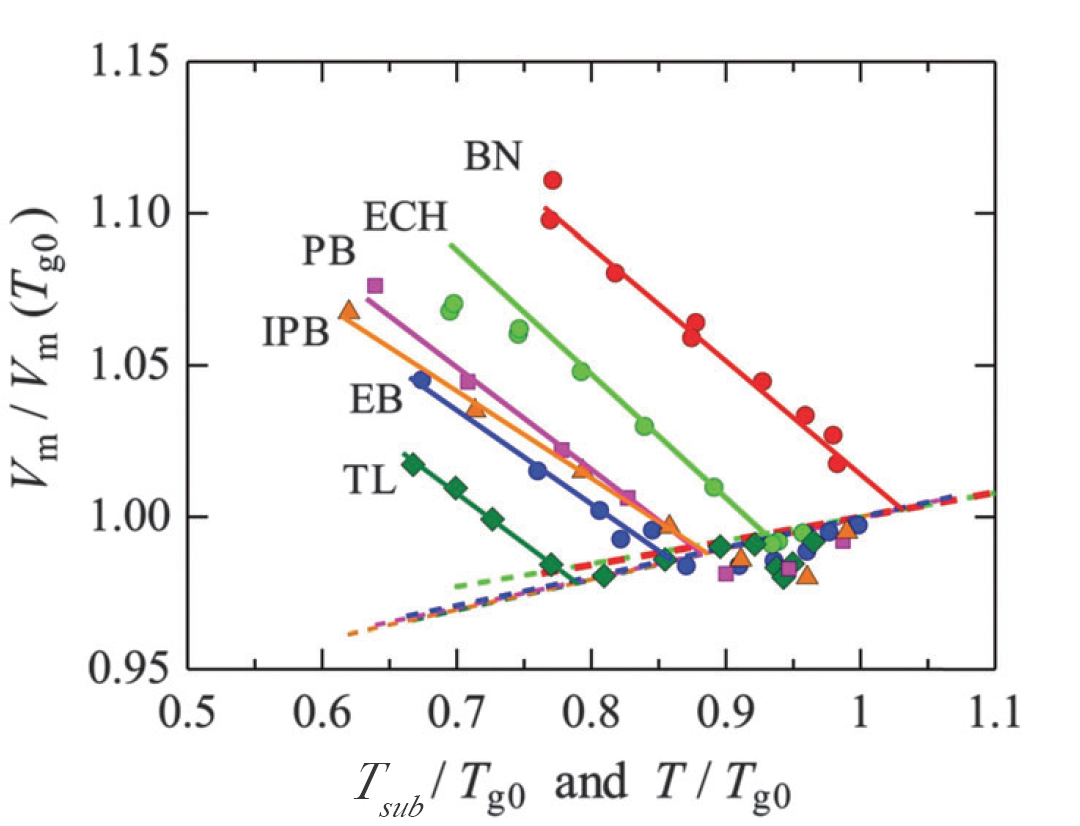
\includegraphics[width=\textwidth]{Density_Vs_Tsub_Ishii.png}
		\caption{}
		\label{fig:IshiiDensityTsub}
	\end{subfigure}
	%Image 2
	\begin{subfigure}[htbp]{0.75\textwidth}
		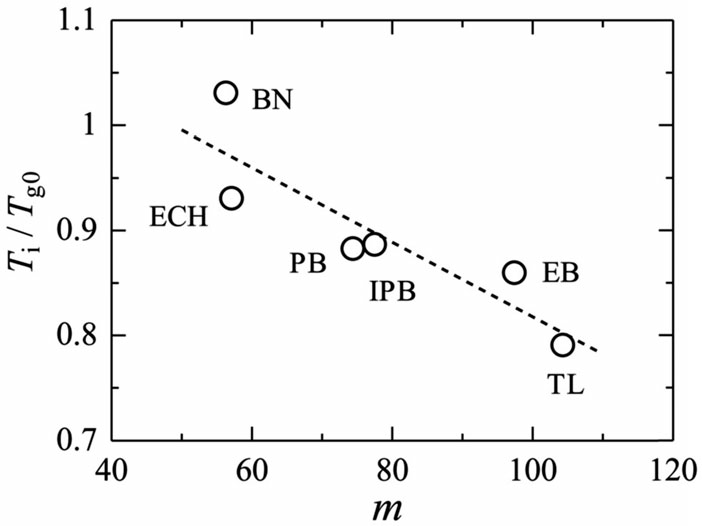
\includegraphics[width=\textwidth]{IshiiMTg.png}
		\caption{}
		\label{fig:IshiiMTg}
	\end{subfigure}
	\caption[(a) Relationship between normalised substrate temperature ($T_{sub}/T_{g0}$) and normalised molar volume ($V_{m}/V_{m} (T_{g0})$) for several \acrshort{vd} molecular glasses showing the greatest density occurs near the intersection of the \acrshort{vd} glasses and their extrapolated \acrshort{scl} \acrshort{Vm} line. (b) Weak relationship between the normalised intersection temperature ($T_{i}/T_{g0}$) found in (a) and the glass \acrfull{m}.]{(a) Relationship between normalised substrate temperature ($T_{sub}/T_{g0}$) and normalised molar volume ($V_{m}/V_{m} (T_{g0})$) for several \acrshort{vd} molecular glasses showing the greatest density occurs near the intersection of the \acrshort{vd} glasses and their extrapolated \acrshort{scl} \acrshort{Vm} line. (b) Weak relationship between the normalised intersection temperature ($T_{i}/T_{g0}$) found in (a) and the glass \acrfull{m}. (a) Modified from \cite{Ishii2014} and (b) Reproduced from \cite{Ishii2014}.}%global caption
	\label{fig:IshiiTsubM}
\end{figure}


The Ishii and Nakayama \cite{Ishii2014} and Nakayama, et al. \cite{Nakayama2013} glass relationship between \gls{Tsub} and \gls{Vm} is presented in Figure \ref{fig:IshiiTsubM}. In Figure \ref{fig:IshiiDensityTsub} the \gls{Tsub} for several molecular glasses are plotted against the \gls{Vm}, both normalised by the quench glass' \gls{Tg} and \gls{Vm}, called \acrshort{Tg0} and \gls{Vm} (\acrshort{Tg0}) respectively. The plot shows the \gls{vd} glass' densities increases with \gls{Tsub}, several being able to achieve enhanced density as per the condition $V_{m}/V_{m} (T_{g0})<1.0$. The densest glasses occur near the \gls{Ti} between the solid \gls{vd} glass trend line and an extrapolated \gls{scl} \gls{Vm} line. Figure \ref{fig:IshiiMTg} shows a weak relationship between this highest density state at $T_{i}/T_{g0}$ and \gls{m}, similar to the one found by Yu, et al. \cite{Yu2013} between $\delta T_{g}/T_{g}$ and m in Figure \ref{fig:YuMTgPlot}. Suggesting high \gls{m} glasses show the greatest promise for increased density, and that \glspl{smg} will have modest enhanced density relative to tradition \glspl{bmg} \cite{Ishii2014, Nakayama2013}. 

Aji, et al. \cite{Aji2013} provides the only density data on \glspl{smg} showing a modest density increase of 0.5\% relative to traditional quenched \gls{bmg}. In contrast Guo, et al. \cite{Guo2012} work has shown polymer \glspl{usg} display a significant reduction in density coupled with \gls{dTg}, though they point out this is the opposite of molecular and other \glspl{usg}. 

\subsubsection{Indentation Modulus ($M$)}
The \gls{M} of a material is an elastic constant which accounts for compressive and shear deformations with compressive load. It is given by;

\begin{equation}
M \equiv 
\frac{E}
{1-\nu^{2}}
\label{equ:IndentModulus}
\end{equation}

The initial work of Yu, et al. \cite{Yu2013} has found a modest increase in \gls{M} for \glspl{smg} over \glspl{bmg} of $5- 10\%$ for the ultrastable \ZrCuAl~ system, indicating \gls{smg} may be able to better support compressive loads. \todo{Assuming this based on the definition.}

\subsection{SMG Structure, Medium Range Order (MRO)} \todo{Normal Glasses only has SRO Crystals have LRO (Donald S. of MIT) So MRO is not a typical situation.}
From molecular glasses it is expected \glspl{usg} will be distinguishable from normal glasses by extra-low angle peaks in \gls{xrd} analysis. However Yu, et al. \cite{Yu2013} have observed this is not the case with \glspl{smg} as the analysis appears identical to \glspl{bmg}, implying \glspl{smg}' corresponding states of packing are not significantly different. This difficultly was also encountered by Aji, et al. \cite{Aji2013} whom were also unable to differentiation between ordinary and ultrastable glass by \gls{xrd} and \gls{hrtem}. However Yu, et al. \cite{Yu2013} went on to suggest there may be a hidden polyamorphous or layer-like super-structures in the \glspl{smg}, although they were unable to confirm it. 

Using \acrshort{stem} techniques Aji, et al. \cite{Aji2013} were able to identify \gls{mro} structures of 2nm in their \ZrCuNiAl~ \gls{smg}, which they believe are responsible for the ultrastable effects. Via \gls{abed} Aji, et al. \cite{Aji2013} examined the \gls{mro} further and found it is not composed of any of the alloy's known simple crystal structures, but are instead distorted icosahedra with local crystal-like cube symmetry. Aji, et al. \cite{Aji2013} believe this \gls{mro} is responsible for the \gls{smg} stability characteristics and offers explanation for why only \gls{vd} techniques can produce \gls{smg}. The \gls{mro} occurs when tens to hundreds of atoms are arranged in the energy minima, but do not form in ordinary glass because solidification from liquid, or annealing already formed glass at elevated temperature, does not allow sufficient time for \gls{mro} formation. Conversely the slow \gls{vd} techniques used in forming \glspl{usg} allows the surface atoms to arrange themselves into the highly order \gls{mro} structures before being covered by later arriving atoms. \todo{Think 3D printing layering.}

\subsection{Potential SMG Challenges}
Investigation has identified potential issues and challenges with the demonstrated \gls{pvd} pressures and \gls{Tsub} required when producing \glspl{smg}. For example, Qin, et al. \cite{Qin2009} has found in the binary amorphous Zr$_{65}$Cu$_{35}$ system raising substrates to just room temperature can cause crystallisation of films if the Ar pressure is not properly refined. This appears concerning as the alloy constituents of this system are in comparable amounts with the Yu, et al. \cite{Yu2013} and Aji, et al. \cite{Aji2013} systems of \ZrCuAl~ and \ZrCuNiAl~ respectively. Additionally Aji, et al. \cite{Aji2013} found more simple binary and ternary system \glspl{smg} were more difficult to produce, had more modest gains in \gls{Tg} and \gls{Tx}, and often contained crystalline phases. However these findings support the theory simple atomic structure metallic alloys may not be suitable to form \glspl{smg}, and it may be only more atomically complicated \glspl{bmg}, such as high \gls{gfa} ternary systems, are suitable to form \glspl{smg} \cite{Yu2013}. As this research will be working with ternary Mg systems, it is believed they will be sufficiently atomically complicated to form \glspl{smg}. 

It is known from Liu, et al. \cite{Liu2012} and Cao \cite{Cao2013} that higher deposition rates result in smoother \glspl{tfmg}, while Kearns, et al. \cite{Kearns2008} work with molecular \glspl{usg} has found lower deposition rates produce more kinetically stable, lower enthalpy glasses. The effects of deposition rate on \gls{smg} production were not examined by Yu, et al. \cite{Yu2013}, Aji, et al. \cite{Aji2013}, and Wang, et al. \cite{Wang2014}, but there was a significant difference in deposition rate used by the three groups. Both Aji, et al. \cite{Aji2013}, and Wang, et al. \cite{Wang2014} made use of very slow deposition rates of less than 0.2nm/s to produced their \glspl{smg} with both materials displacing the ideal behaviour of high kinetic stability coupled with low enthalpy. However Yu, et al. \cite{Yu2013} made use of deposited rate almost a magnitude higher, 1.4nm/s and produced an \glspl{smg} possessing both high kinetic stability and high enthalpy. As Yu, et al. \cite{Yu2013} and Aji, et al. \cite{Aji2013} had similar \glspl{smg} of \ZrCuAl~ and \ZrCuNiAl~ respectively, these observations would suggest it may be possible to produce lower enthalpy \glspl{smg} by lowing the deposition rates, although if the \gls{tfmg} trends hold the films may become more rough. These effects should be examined in new research as there is no body of work on varying \gls{smg} deposition rate and the reliability of \gls{tfmg} trends has not been confirmed to translate to \gls{smg} systems. 

Interestingly Schlüter, et al. \cite{Schluter2012} have already examined the MgZnCa system (Mg$_{45}$Zn$_{50}$Ca$_{5}$ and Mg$_{60}$Zn$_{35}$Ca$_{5}$) over various power and deposition rates to produce thin films. They found high power/deposition rates result in crystalline films while lower rates are able to deposit fully amorphous \todo{Would even slower rates produce SMG? Check their parameters again.} \gls{tfmg} \cite{Schluter2012}. They came to the conclusion the higher powers allow sufficient heat to be added to the substrate for crystallisation to occur \cite{Schluter2012}. Wang, et al. \cite{Wang2014} found similar results working with Au$_{52}$Ag$_{5}$Pd$_{2}$Cu$_{25}$Si$_{10}$Al$_{6}$ \gls{smg} where they showed the heat additions of the magnetron sputtering plasma can be attributed to a 20K temperature fluctuation at the substrate. This alloy has a fairly low \gls{Tg} of 400K meanings its ideal \gls{Tsub} for \gls{smg} deposition is around room temperature, making these 5\% of \gls{Tg} fluctuations significant. Additionally MgZnCa based bio-alloys have a similar low \gls{Tg} (405K for \MgZnCa~ \cite{Cao2013b, Gu2005}) suggesting their substrates can be expected to experience the same 20K temperature fluctuation. 

These findings raise important question as to how high deposition power can be in the Mg system without the risk of elevated \gls{Tsub} exceeding the ideal range and resulting in \gls{tfmg} or crystalline films instead \gls{smg} films. Can \gls{smg} deposition power parameters be refined to the point that no substrate heat addition is needed to produce ultrastable materials, or that substrates will needed to be cooled These are significant as the implications suggest a possibility of reduced production cost through higher production rates, and reduced energy use. 
 
\subsection{Thin Film Testing Methods}
\subsubsection{Adhesion}
Scratch tests can be used to ascertain the film adhesion. 
The adhesion of films is readily tested by scat methods \cite{Bull1996, Burnett1987, Burnett1988, Pan2010}.

\section{Biomedical Materials} \todo{Outline for biomaterials
	-Human Body bio-compatibility requirements
	-Current bio-material limitations
	-Constant elements rolls in body
	-Corrosion
	-Hydrogen evolution
	-Pitting corrosion
	-Cell viability testing?}
\subsection{Introduction}
Biomaterials are materials designed for use within a human or other animal's body for a medical purpose. This task requires the materials to be biocompatible, which is taken to mean they must not adversely affect the body. Generally this requirement has been met by the use of bio-inert materials like Ti or certain polymers which do not interact with the body and do not significantly degrade or corrode. After these bio-inert materials have served their function, they often have to be removed via secondary surgeries. 

\subsection{Biomaterial Requirements} 
In vivo biomaterials are medical devices designed to aid in healing by performing part of the body's internal functions. They are approved and tested by regulatory organisations like the \gls{fda} in the USA, and the \gls{tga} in Australia. To gain approval devices are subjected to a series of biocompatibility tests which establish the body's acceptance to them in the surrounding tissues and the body as a whole. Actual passing requirements are dependent on the consequence of failure (i.e. heart values have stringent requirements as failure can result in death), but as minimal requirements, \textit{in vivo} medical device treatment should not result in any of the following:

%Bullet List
\begin{itemize}
	\item Irritate the surrounding structures;
	\item Provoke an abnormal inflammatory response;
	\item Incite allergic or immunologic reactions; or
	\item Cause cancer. 
\end{itemize}

\subsubsection{Current Metallic Biomaterials}
\todo{Make sure you a paragraph on polymers and ceramics to ensure the lit rev is thorough}
Traditional metallic biomaterials like stainless steels and Ti are designed to be bio-inert and not degrade within the body. After severing their function they must be removed via secondary surgeries unless they have been designed to remain in the body permanently. There is also a significant mismatch between their high stiffness and strength relative to bone, which in orthopaedic applications can result in stress shielding.

Stress shielding is a reduction in bone density and strength which results from reduced stimulus during bone remodelling. It occurs around orthopaedic implants because they are able to carry significant loads and thus the bones are not thoroughly stimulated. Mg implants are less sustainable to this phenomena because their \gls{E} is only about $41 - 45~ GPa$, which is much closer to human bone's $3 - 20~ GPa$ than other metallic biomaterials \cite{Wang2012, Zberg2009}.

\subsubsection{Metallic Biochemistry}
Essential bio-absorbable metallic elements are critical for proper bodily function and when metabolised can aid in the healing process. This makes the elements of Mg, Zn, and Ca ideal major alloy constituents for biodegradable alloys. Moreover, as these elements are water soluble any reasonable excess can be safely excreted from the body via urination.

Mg plays a critical role in numinous reactions within the body. It is an activator in many enzyme reactions, co-regulator in protein synthesis and muscle contraction, and stabiliser of RNA and DNA \cite{Zheng2014} . In the past, when used as an \textit{in vivo} biomaterial Mg has also been linked to stimulating new bone growth \cite{Witte2010}. \todo{Review article reference. Go back and add in the original reference later.} Zn is a trace element in the body which appears in enzyme classes and in muscles \cite{Zheng2014}. \todo{Should be additional sources to back this.} Ca is well known for its structure function in the skeleton, but also has a signal function in muscle contractions, blood clotting, and cell function \cite{Zheng2014}. Other essential minerals which can be safely used in bio-absorbable alloys include Fe and Mn.

Other elements like Al and \glspl{re} have also been alloyed with Mg in past, but their use is not ideal as they are known to not meet the necessary biomaterial requirements. For example, Al has been linked to neurological disorders such as Alzheimers disease \cite{Zheng2014}. Even though the body can tolerate toxic elements in small quantities it is not ideal, and they will not be considered for bio-corrosion applications in these works. 

\subsection{Degradation of Biomaterials} 
Ideally essential metallic element biodegradable alloys are designed to undergo controlled corrosion \textit{in vivo} throughout the tissue healing process. This gradually releases corrosion products around the injury site throughout the healing process, which are either metabolised to assist with the healing or simply excreted. Once healing is complete the support of the biodegradable alloys is no longer needed. The materials continue to degrade ultimately corroding completely to leave no implant residues, and eliminating the need for secondary removal surgeries. 

\subsubsection{Basic Theory of Corrosion and Its Measurement}
Corrosion is an electrochemical reaction describing the flow of electrons which occurs when a physical electrical connection exist between an anode and a cathode via an electrolyte medium. By convention, electrons will flow from the negative anode to the positive cathode, \todo{Anode and Cathode charges are opposite to Sputtering because this reaction releases voltage, like a battery, while sputtering draws voltage.} resulting in oxidation at the anode and reduction at the cathode. 

The kinetics of the corrosion reaction acting upon a specimen can be measured by \gls{pdp} scans, in which the rate of the anodic or cathodic reactions on the specimen (i.e. the working electrode) are represented by the current density (i.e. current per unit area). The rate of the corrosion reaction can be significantly affected by numerous variables including temperature, specimen surface condition \cite{Jones1992}, and the chemical environment and thus these should be carefully controlled and standardised. 

The polarisation scans are performed by controlling the anodic or cathodic reactions' driving force, AKA their \gls{Vp}, and observing the applied \gls{i} required to produce the desired variations in potential. The anodic scans start at low potentials and ramp up, whereas the cathodic start at high potentials and ramp down, hence by convention anodic currents are positive and cathodic negative. \todo{May not be the reason. May have to do with electron flow. Re-read Jones Chapter 3 to see what it says.} The slowest corrosion rate will occur when the anodic and cathodic currents equal each other and the applied current density is at its minimum (theoretically zero); this is known as the \gls{ocp}. 

The Tafel equation (Equation \ref{equ:Tafel}) and Tafel Plots are tools used to interpret the data generated by \gls{pdp} scans. The Tafel equation expresses the anodic or cathodic reactions' current density as a function of their \gls{nOver}; overpotential being defined as the difference between the \gls{Ea} and \gls{ocp} (\acrshort{Eocp}).

\begin{equation}
\eta = E_{A} - E_{OCP}=\beta log \frac{i}{i_{0}}
\label{equ:Tafel}
\end{equation}

Where \acrshort{B} is the Tafel slope, \acrshort{i} the applied current density, and \acrshort{i0} the exchange current density. 

Plotting the Tafel equation for both the anodic and cathodic reactions produces the Tafel Plot (Figure \ref{fig:EnosTafel}) for the corrosion reaction. From the plot the \gls{ocp}, where anodic and cathodic currents are equal, can be obtained by extrapolation. This is performed along the linear region of the anodic and cathodic \acrshort{B} slopes, with the extrapolations' intersection indicating the \gls{ocp}. The current density and potential coordinates of the \gls{ocp} on the plot indicate the \gls{icorr}, and \gls{Ecorr} for the reaction. When evaluating improved corrosion resistance the idea specimen will have both a more noble potential (i.e. \gls{Ecorr} is more cathodic), \todo{i.e. The Potential is a larger number ( -1.0 V < -0.5 V)} and a reduced \gls{icorr} in relation to the comparison specimen.

%single image
\begin{figure}[htb]
	\centering
	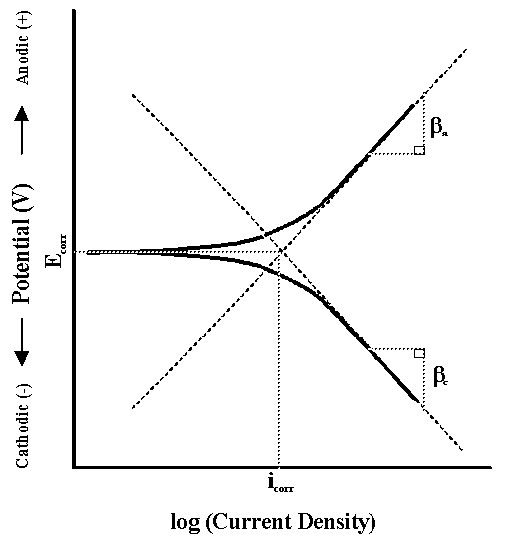
\includegraphics[width=0.75\textwidth]{Enos_TafelPlot.png}
	\caption[Tafel Plot showing the positive anodic Tafle slope $\beta_{a}$ negative cathodic Tafle slope $\beta_{c}$, and their linear extrapolations with their intersection indicating the \acrshort{ocp}, and thus the \acrshort{icorr} and the \acrshort{Ecorr} positions.]{Tafel Plot showing the positive anodic Tafle slope $\beta_{a}$ negative cathodic Tafle slope $\beta_{c}$, and their linear extrapolations with their intersection indicating the \acrshort{ocp}, and thus the \acrshort{icorr} and the \acrshort{Ecorr} positions. Adapted from \cite{Enos1997}.}
	\label{fig:EnosTafel}
\end{figure}

\subsubsection{Mg Hydrogen Evolution}
The corrosion of Mg (equation \ref{equ:MgH}) results in the generation of molecular hydrogen gas products, in a process called hydrogen evolution \cite{Zberg2009}. This is problematic in biomedical applications as biodegradation of Mg alloys can result in the production of hydrogen gas cavities around the treatment area. 

As noted in the Witte \cite{Witte2010} historical review of Mg implant clinical trials, generally these gas cavities were not considered painful and often subsided within days or weeks, with complete corrosion of implants following shortly \cite{Verbrugge1933, Lambotte1932}. The corrosion of the implants also did not appear to harm the surrounding tissues, showing no signs of irritation or inflammation \cite{Verbrugge1933}. Though excessive gas formation produced local swelling and significant pain, resulting in implants being prematurely removed \cite{Lambotte1932}. The cause of these critical failures were soon identified as resulting from the large potentials of electrically coupling Mg with Fe, and were not repeated \cite{Lambotte1932}. 

\begin{equation}
Mg + 2H_{2}O \rightarrow Mg^{2+} + 2OH^{-} + H_{2}
\label{equ:MgH}
\end{equation}

As can be inferred from equation \ref{equ:MgH}, the severity and quantity of H$_{2}$ gas generation via hydrogen evolution is dependent on the corrosion of the Mg. Thus the effects of hydrogen evolution can be greatly mediated by slowing the rate at which H$_{2}$ gas is generated by lowing the corrosion rate of Mg. Common methods employed to improve and inhibit Mg corrosion include the use of high-purity Mg alloys, alloying to promote the formation of protective passive films, and alloying to promote the formation of amorphous structures. 

In devolving high corrosion resistance Mg alloys, Wang, et al. \cite{Wang2012} have found amorphous and semi-crystalline Mg$_{67}$Zn$_{28}$Ca$_{5}$ \todo{Very similar alloy. Thus trend should hold for Mg65Zn30Ca5} alloy are able to quickly form a protective passive film to limit their corrosion rate and hydrogen evolution. Initially these alloys produce a moderate amount of H$_{2}$ gas, but the rate quickly drops off and results in a very small amount of total gas being release throughout the corrosion process \cite{Wang2012}. In contrast, the fully crystalline alloy initially sees its H$_{2}$ gas release rate increase over time, before eventually reducing and stabling at a low level \cite{Wang2012}. This occurs because initially it is difficult for the crystalline alloy to form the passive film, resulting in a high average rate and large total volume of gas release \cite{Wang2012}. The release of large total amounts of hydrogen gas is closely linked to great amounts of specimen weight loss, meaning these crystalline alloys loss far more bulk material to the corrosion process than the amorphous ones, and hence would have shorter service lives \cite{Wang2012}. 

Zberg, et al. \cite{Zberg2009} has also been particularly successful at reducing hydrogen evolution with amorphous Mg$_{60+x}$Zn$_{35-x}$Ca$_{5}$ alloys, showing the passive films generated by Zn can eliminate hydrogen evolution almost completely. From these studies, Zberg, et al. \cite{Zberg2009} showed Zn poor alloys produce significant hydrogen, while alloys with Zn contents greater than 28at\% produced almost none. Additionally Zberg, et al. \cite{Zberg2009} conditioned animal trials on pigs of their alloys via implanting Mg disk of amorphous Mg$_{60}$Zn$_{35}$Ca$_{5}$ and crystalline Mg alloy (WZ21) within the abdominal walls for a period of three months. The wound-healing process was characterised as typical for both alloys with no inflammatory reactions observed for either \cite{Zberg2009}. Though only the crystalline alloy implants showed hydrogen generation during the conducted one and three month examinations \cite{Zberg2009}.

%single image
\begin{figure}[htbp]
	\centering
	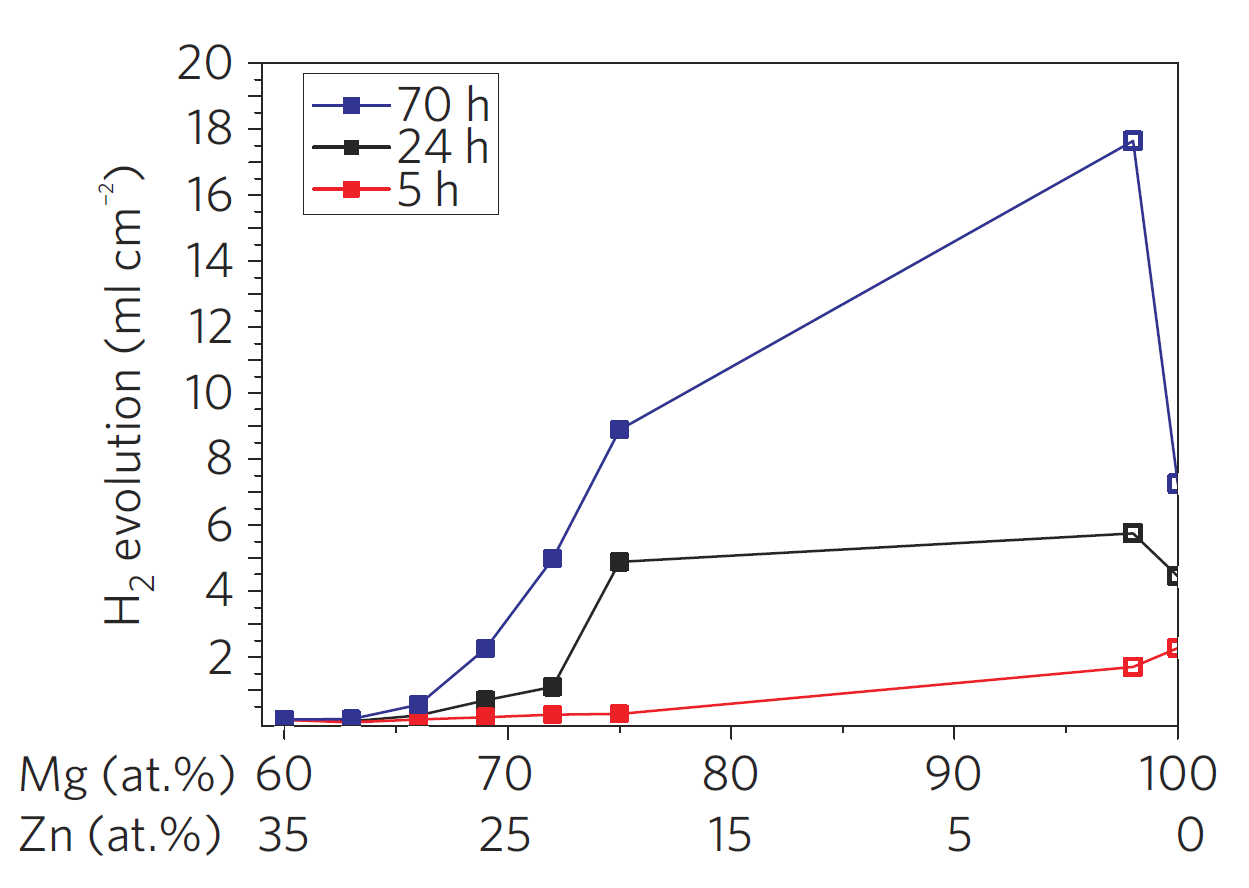
\includegraphics[width=0.75\textwidth]{ZbergHydrogen.png}
	\caption[Plot of hydrogen evolution generated by Mg$_{60+x}$Zn$_{35-x}$Ca$_{5}$ alloys. Note the hydrogen evolution drops off significantly for Zn concentration $>28at\%$. (Filled points are amorphous, open crystalline).]{Plot of hydrogen evolution generated by Mg$_{60+x}$Zn$_{35-x}$Ca$_{5}$ alloys. Note the hydrogen evolution drops off significantly for Zn concentration $>28at\%$. (Filled points are amorphous, open crystalline). Reproduced from \cite{Zberg2009}.}
	\label{fig:ZbergHydrogen}
\end{figure}

As Witte \cite{Witte2010} has shown in his review magnesium was showing promise as a bio-reabsorbable material in the early 1900s before the trend switch to bio-inert materials like Ti. 

The challenges with bio-reabsorbable metals is currently a need to;

%Bullet List
\begin{itemize}
	\item Reduce the level of ion toxicity;
	\item Reduce the amount of hydrogen gas; and
	\item Control the loss of mechanical strength over time. 
\end{itemize}

\subsubsection{Pitting Corrosion}
Generally pitting is associated with the breakdown of passive films, such as in stainless steels \cite{Zheng2014, Jones1992, Schweitzer2009}. Pitting is associated with quenched in free volume surface defects in \gls{bmg} \cite{Wang2012}. \todo{Expect pitting may be less in SMGs, because despite higher density being expected, the surface finish may be higher quality with less defects…}

Pitting corrosion is associated with the breakdown of the passive film (Reread page 41 of Jones fundamentals) \cite{Zheng2014, Jones1992, Schweitzer2009}. This can be due to the presents of Cl- ions \cite{Zheng2014}. 

 \Gls{bmg} suffer from pitting corrosion because of quenched in free volume defects \cite{Wang2012} (many more papers. Check later). Pitting increases with level of amorphousness \cite{Schluter2012}. 

Amorphous Mg allows for higher alloy continents and a homogeneous single-phase structure. These help improve corrosion characteristics. 

Amorphous metal has high corrosion resistance due to

%Bullet List
\begin{itemize}
	\item Chemical homogeneity 
	\item Monolithic structure
	\item Lack of grain boundaries 
\end{itemize}
 
Mg and Ca corrode in preference to Zn, leaving behind a Zn rich surface which promotes a passive layer \cite{Wang2012}.
Pitting occur on anodic end of the Tafel Plots \cite{Schluter2012}.

\subsection{Anti-biotic Scaffolds}


%%%%%%%%%%%%%%%%%%%%%%%%%%%%%%%%%%%%%%%%%%%%%%%%%%%%%%%%%%%%%%%%%%%%%%%%%%

\chapter{EXPERIMENTAL PROCEDURE}
\glsresetall

\section{Target Manufacture} \label{sec:TargetManufacture}
The production of thin films by \gls{pvd} requires targets of appropriate composition for the desired film stoichiometry. These master alloy targets are produced by induction melting of pure constituent element ingots.

\subsection{Base Elements}
The \MgZnCa~ master alloy is prepared from pure constituent element ingots of Mg (99.85 wt\%), Zn (99.995 wt\%), and Ca (99.8 wt\%). Each element ingot is polished and filed to removal surface contamination and oxides. The ingots are cut to size on an auto-cutter (Struers Discotom-6) at a feed rate of no more than $0.2~ mm/s$ at $2850 - 3420$ \acrshort{rpm} (Figures \ref{fig:AutoCutter} and \ref{fig:MgIngot}).

%code to put 2 images side by side in a figure
\begin{figure}[htbp]
	\centering
	%Image 1
	\begin{subfigure}[htbp]{0.49\textwidth}
		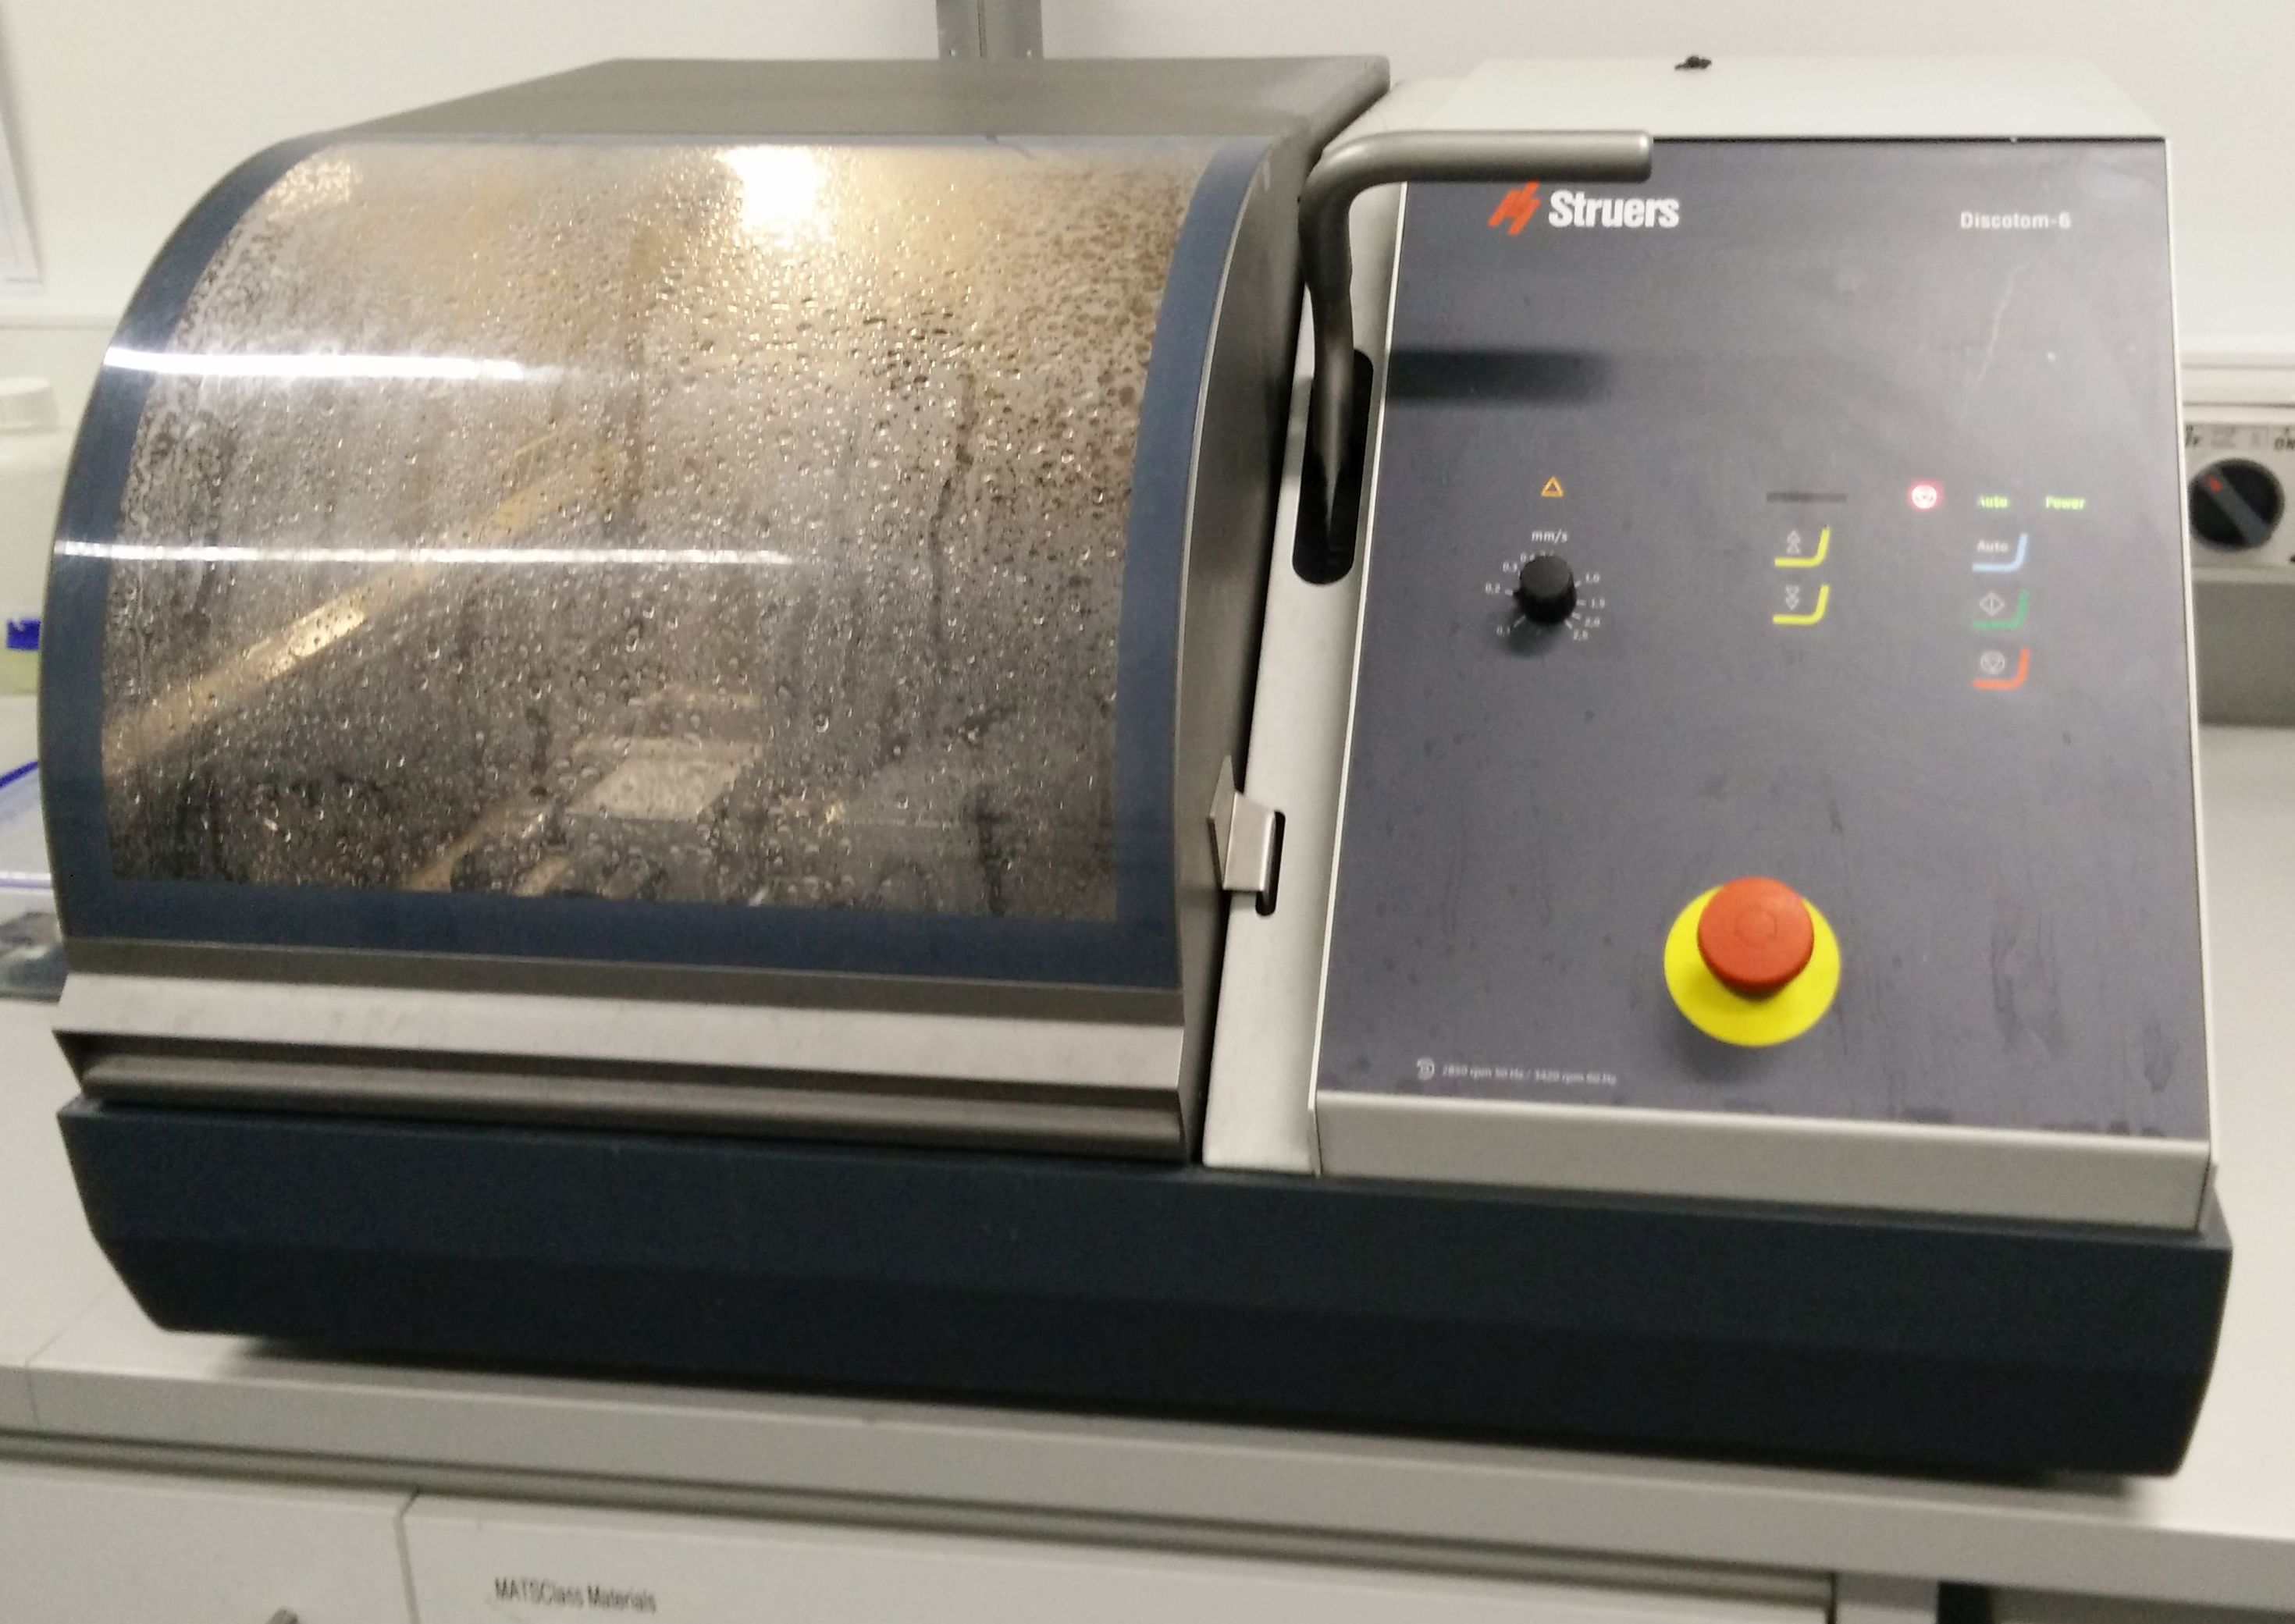
\includegraphics[width=\textwidth]{Ex_AutoCutter.jpg}
		\caption{}
		\label{fig:AutoCutter}
	\end{subfigure}
	%Image 2
	\begin{subfigure}[htbp]{0.30\textwidth}
		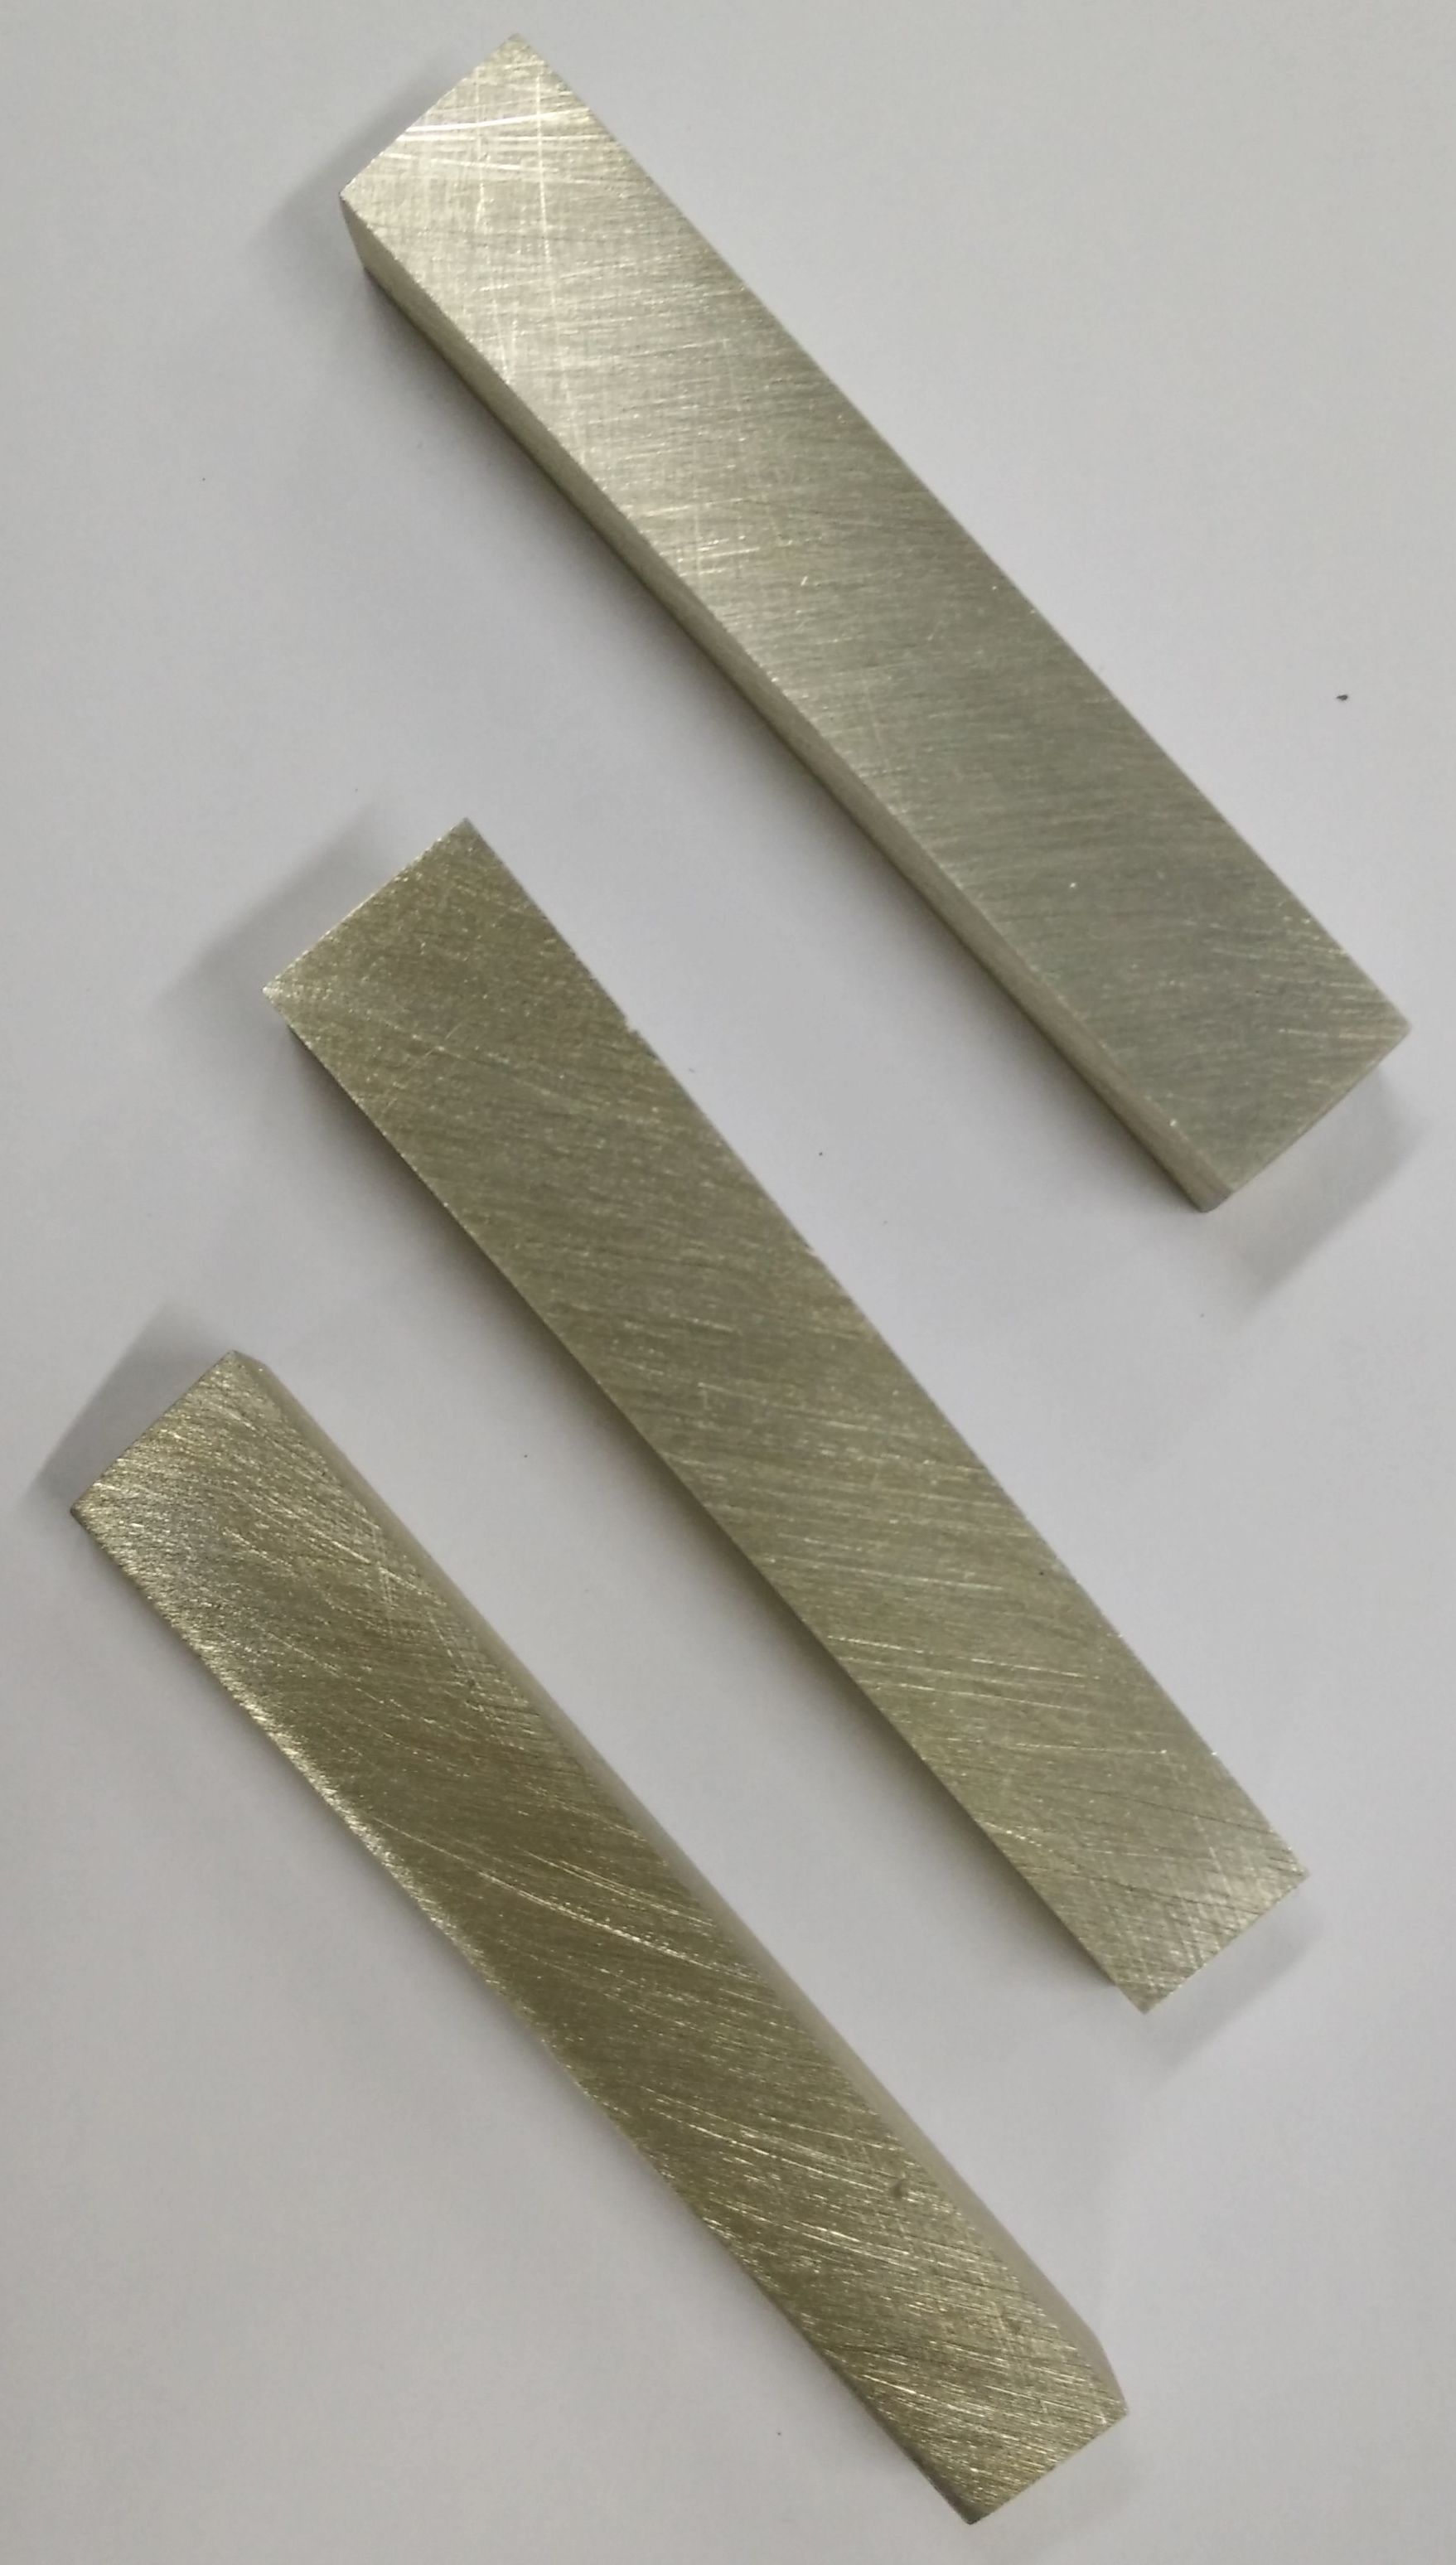
\includegraphics[width=\textwidth]{Ex_Mg_Cut_Ingot.jpg}
		\caption{}
		\label{fig:MgIngot}
	\end{subfigure}
	\caption{(a) Struers Discotom-6 auto-cutter. (b) Cut and fully deoxided Mg ingot ready for casting.}%global caption
	\label{fig:Cutter_MgIngot}
\end{figure}

The total weight of each constituent element required for a master alloy charged is automatically calculated by a developed MS Excel workbook, Figure \ref{fig:ChargeSheet}. This tool auto-computes the required weights of each element from the prepared ingot innovatory, checks the expected master alloy composition, and provides a space for notes on the entire process (i.e. heating cycles, observations, possible future refinements, etc.).

%single image
\begin{figure}[htbp]
	\centering
	\includegraphics[width=0.99\textwidth]{Ex_ChargeSheet.png}
	\caption{Screenshot of the MS Excel workbook developed for auto-calculating master alloy charge weights, checking expected master alloy composition, and taking notes for future refinements.}
	\label{fig:ChargeSheet}
\end{figure}

\subsection{Induction Furnace Melting}
\subsubsection{Induction Furnace Equipment}
The \MgZnCa~ master alloy was prepared from the base element ingots by an in house induction furnace and casting facility (Figures \ref{fig:CastingSchematic} and \ref{fig:LawsCasting}). The facility has a maximum temperature of 1300\degree C, heating rate of 500\degree C/min, and vacuum and dynamic gas melting capability \cite{Laws2007}. The dyanmic gas flow rate can be varied from $0-200~ cm^{3}/min$, and temperature regulated by a K-type thermocouple \cite{Laws2007}. The casting capabilities allow for conventional gravity casting, inverted injection casting, vacuum/suction casting or combination injection/vacuum casting \cite{Laws2007}.

%single image
\begin{figure}[htbp]
	\centering
	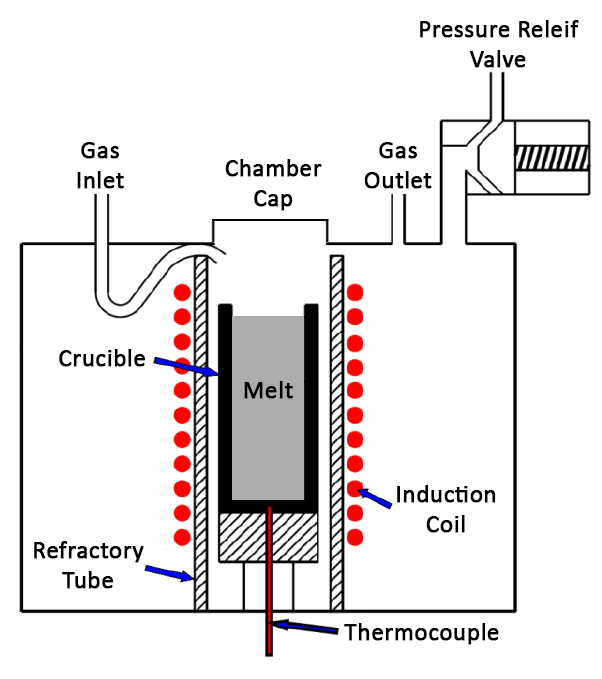
\includegraphics[width=0.75\textwidth]{Ex_Laws_Induction_Schematic.png}
	\caption[Schematic of induction casting melting chamber.]{Schematic of induction casting melting chamber. Adapted from \cite{Laws2007}.}
	\label{fig:CastingSchematic}
\end{figure}

\subsubsection{Crucibles}
Boron nitride coated graphite crucibles were used for the melting because the coating is inert in molten Mg. Two sizes are available for the facility, $32~ mm$ and $34~ mm$ diameter, by $85~ mm$ in length, allowing for melts of $40$ and $60~ cc$ respectively. The Mg and Zn ingots were placed in the bottom of the crucible with maximum wall contact, with the Ca being added on the top, Figure \ref{fig:CrucibleCharge}.

\subsubsection{Melt Cycle}
The crucible was sealed in the induction furnace chamber, evacuated and purged with Ar (99.997 vol.\% purity) five times before starting a continues circulating Ar flow through the camber to prevent oxidation of the melt (Figure \ref{fig:CastingSchematic}). The crucible charge was induction melted at 700\degree C for a couple minutes and stirred with a tungsten rod. The melt was then partially solidification at 385\degree C, remelted and stirred at 650\degree C, partially re-solidification at 385\degree C, and remelted and stirred again at 650\degree C. The melt was then cooled to a casting temperature of $500- 510$\degree C and removed from the melt camber by the incorporated raising bar. This heating/cooling cycle between the alloy's solidus/liquidus region and the liquid state helps ensure a homogeneous alloy melt. 

\subsubsection{Gravity Casting}
For naturally cooled gravity casting the melt was manually poured into a prepared copper plate mould. This mould has spacers allowing for plate thickness ranging from $2~ mm$ to several $mm$, with $4~ mm$ plate proving the most practical (Figures \ref{fig:LawsMould} and \ref{fig:FilledMould}). The $4~ mm$ plate variation has a volume of approximately $20~ cc$ with the riser holding an additional $15.5~ cc$. The mould was prepared by cleaning with lint free paper, polishing with Brasso \textcopyright, and wiping clean again with paper.

%code to put 4 images side by side in a figure
\begin{figure}[htbp]
	\centering
	%Image 1
	\begin{subfigure}[htbp]{0.49\textwidth}
		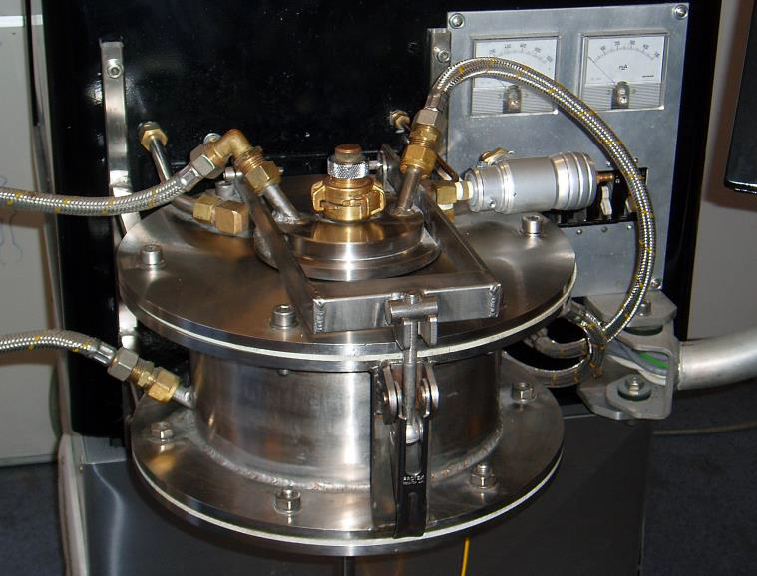
\includegraphics[width=\textwidth]{Ex_LAWS_Induction_Casting.png}
		\caption{}
		\label{fig:LawsCasting}
	\end{subfigure}
	%Image 4
	\begin{subfigure}[htbp]{0.375\textwidth}
		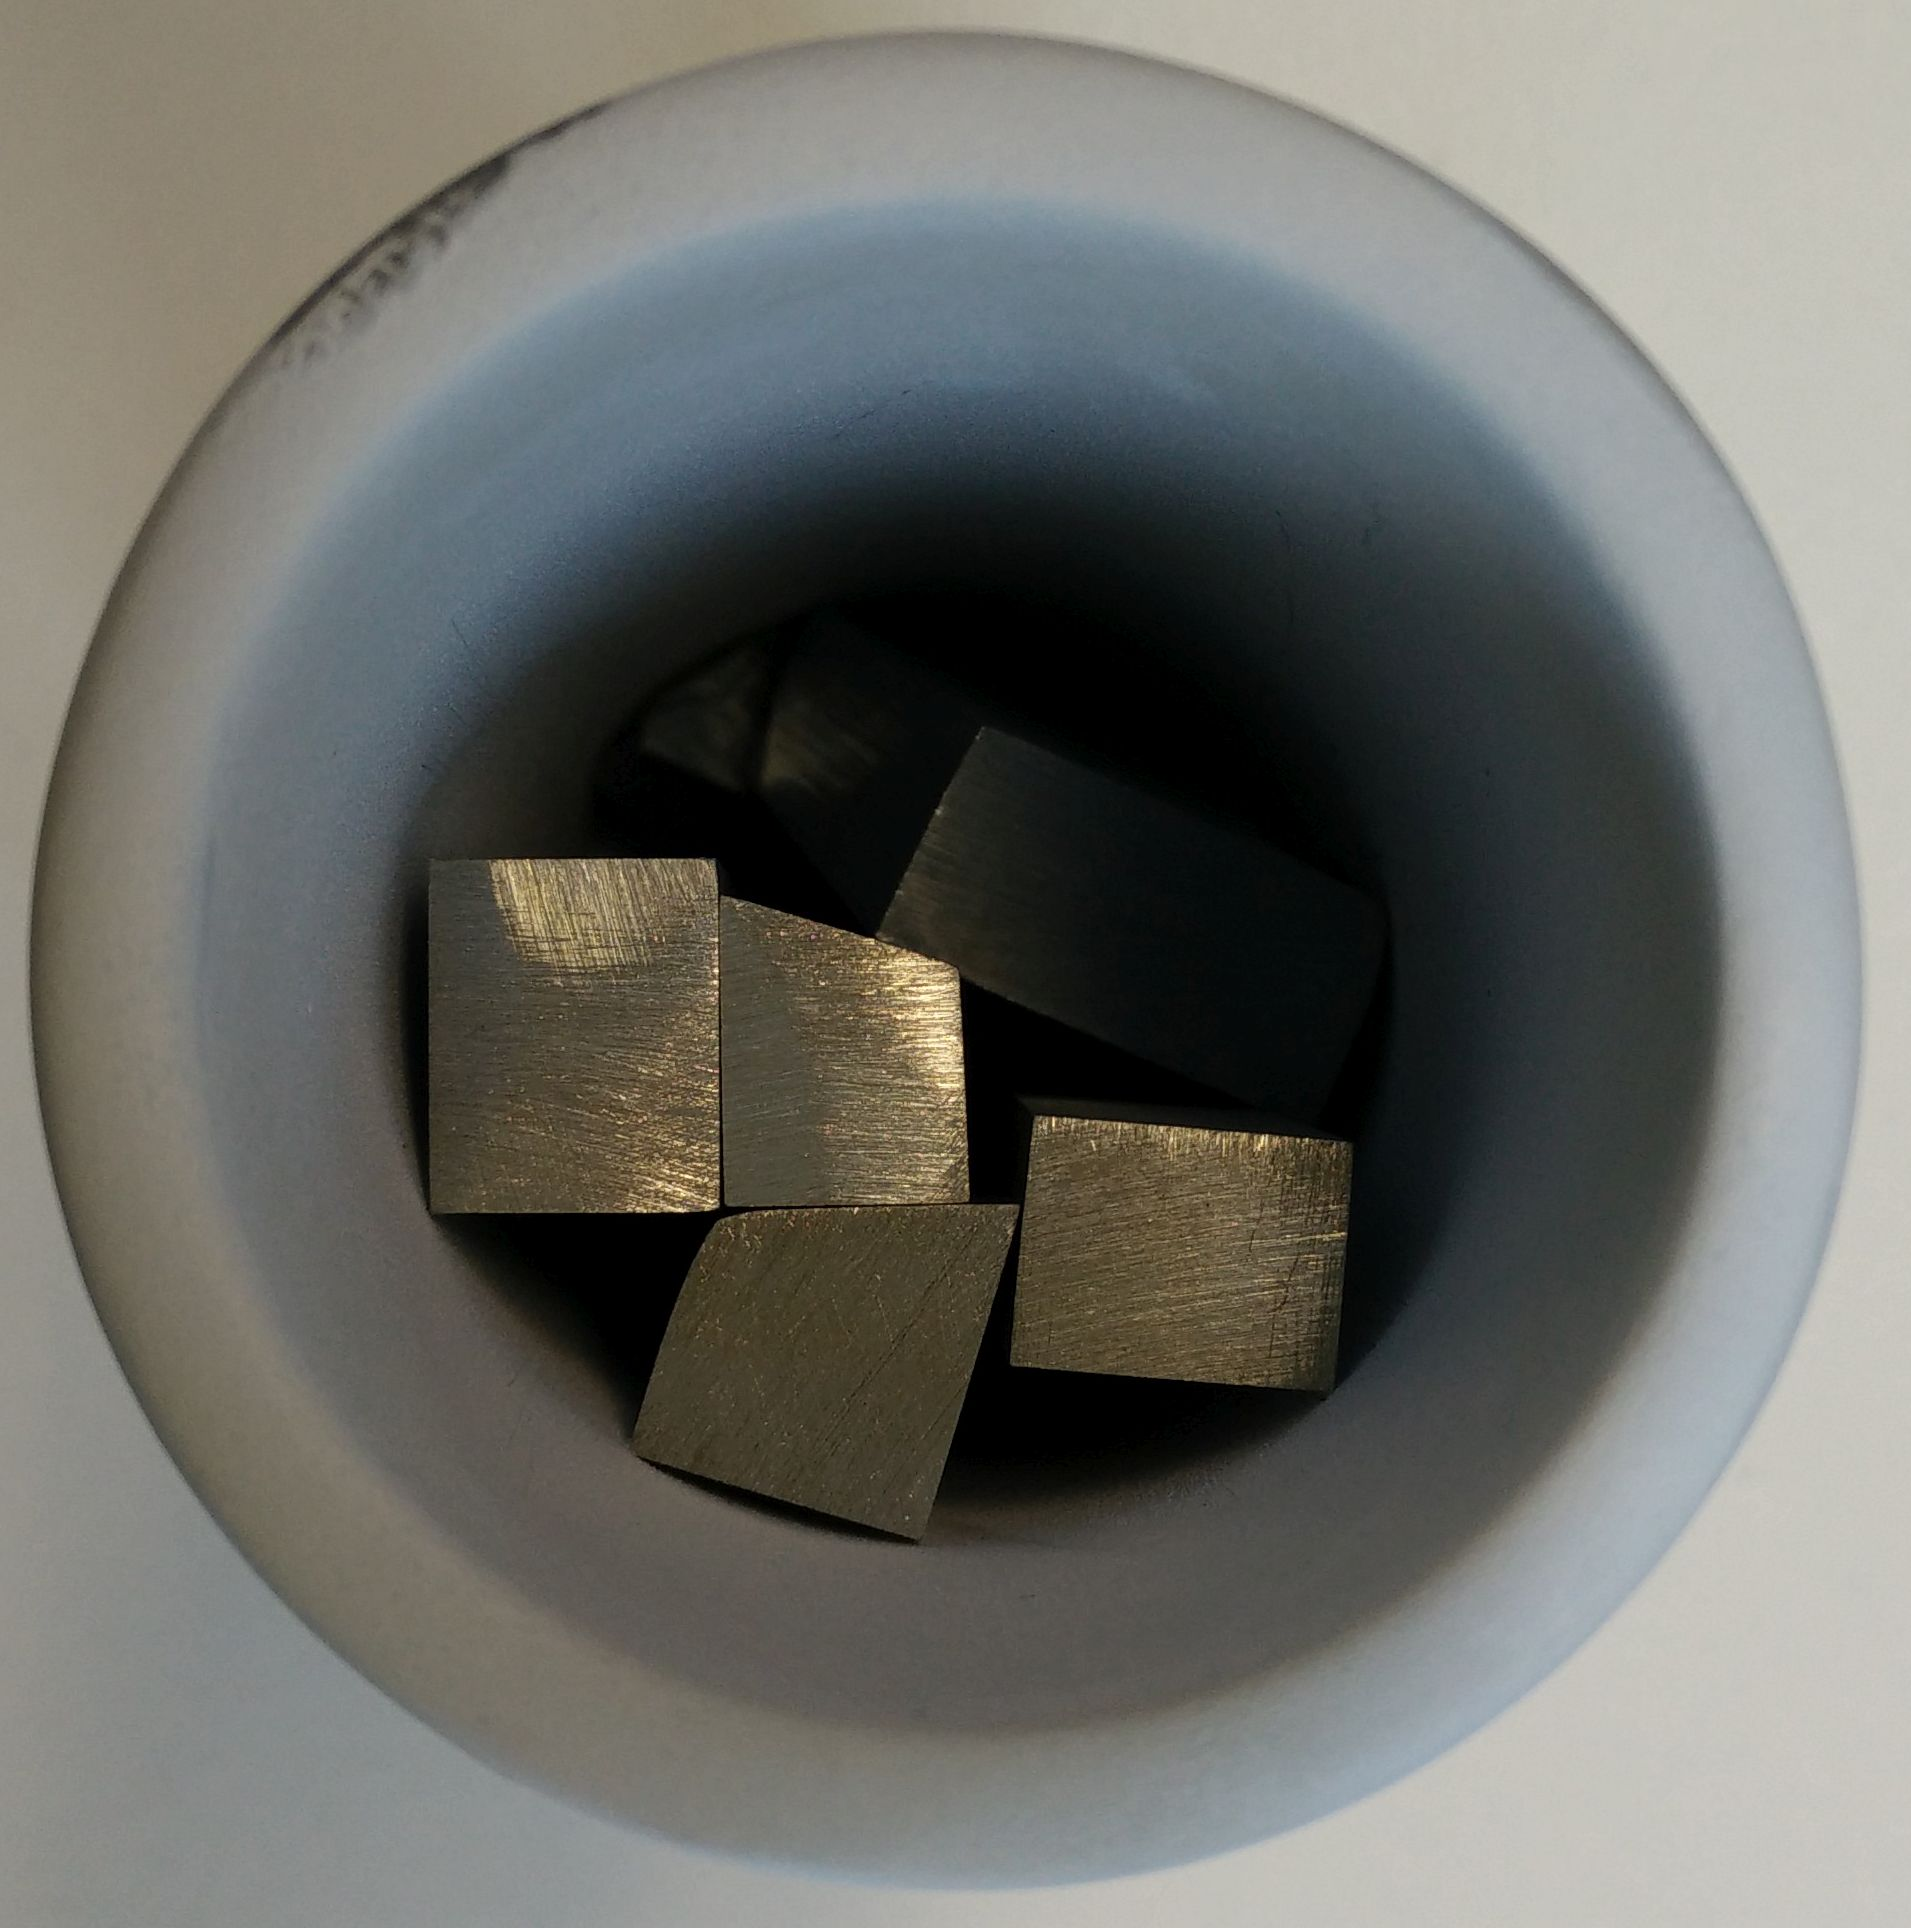
\includegraphics[width=\textwidth]{Ex_Crucible_Charge.jpg}
		\caption{}
		\label{fig:CrucibleCharge}
	\end{subfigure}
	%Image 2
	\begin{subfigure}[htbp]{0.41\textwidth}
		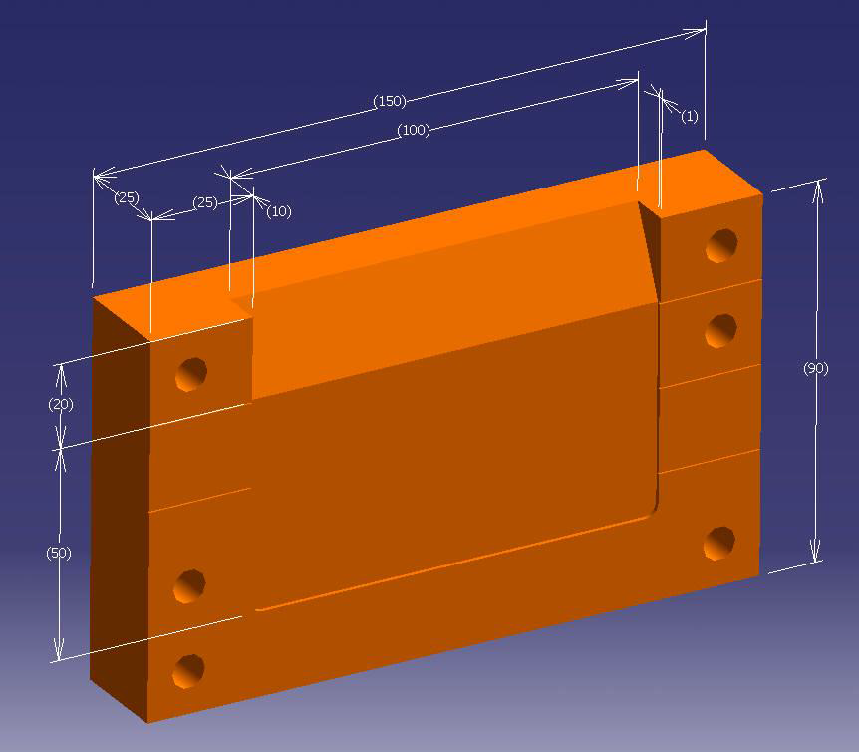
\includegraphics[width=\textwidth]{Ex_Laws_Copper_Mould.png}
		\caption{}
		\label{fig:LawsMould}
	\end{subfigure}
	%Image 3
	\begin{subfigure}[htbp]{0.49\textwidth}
		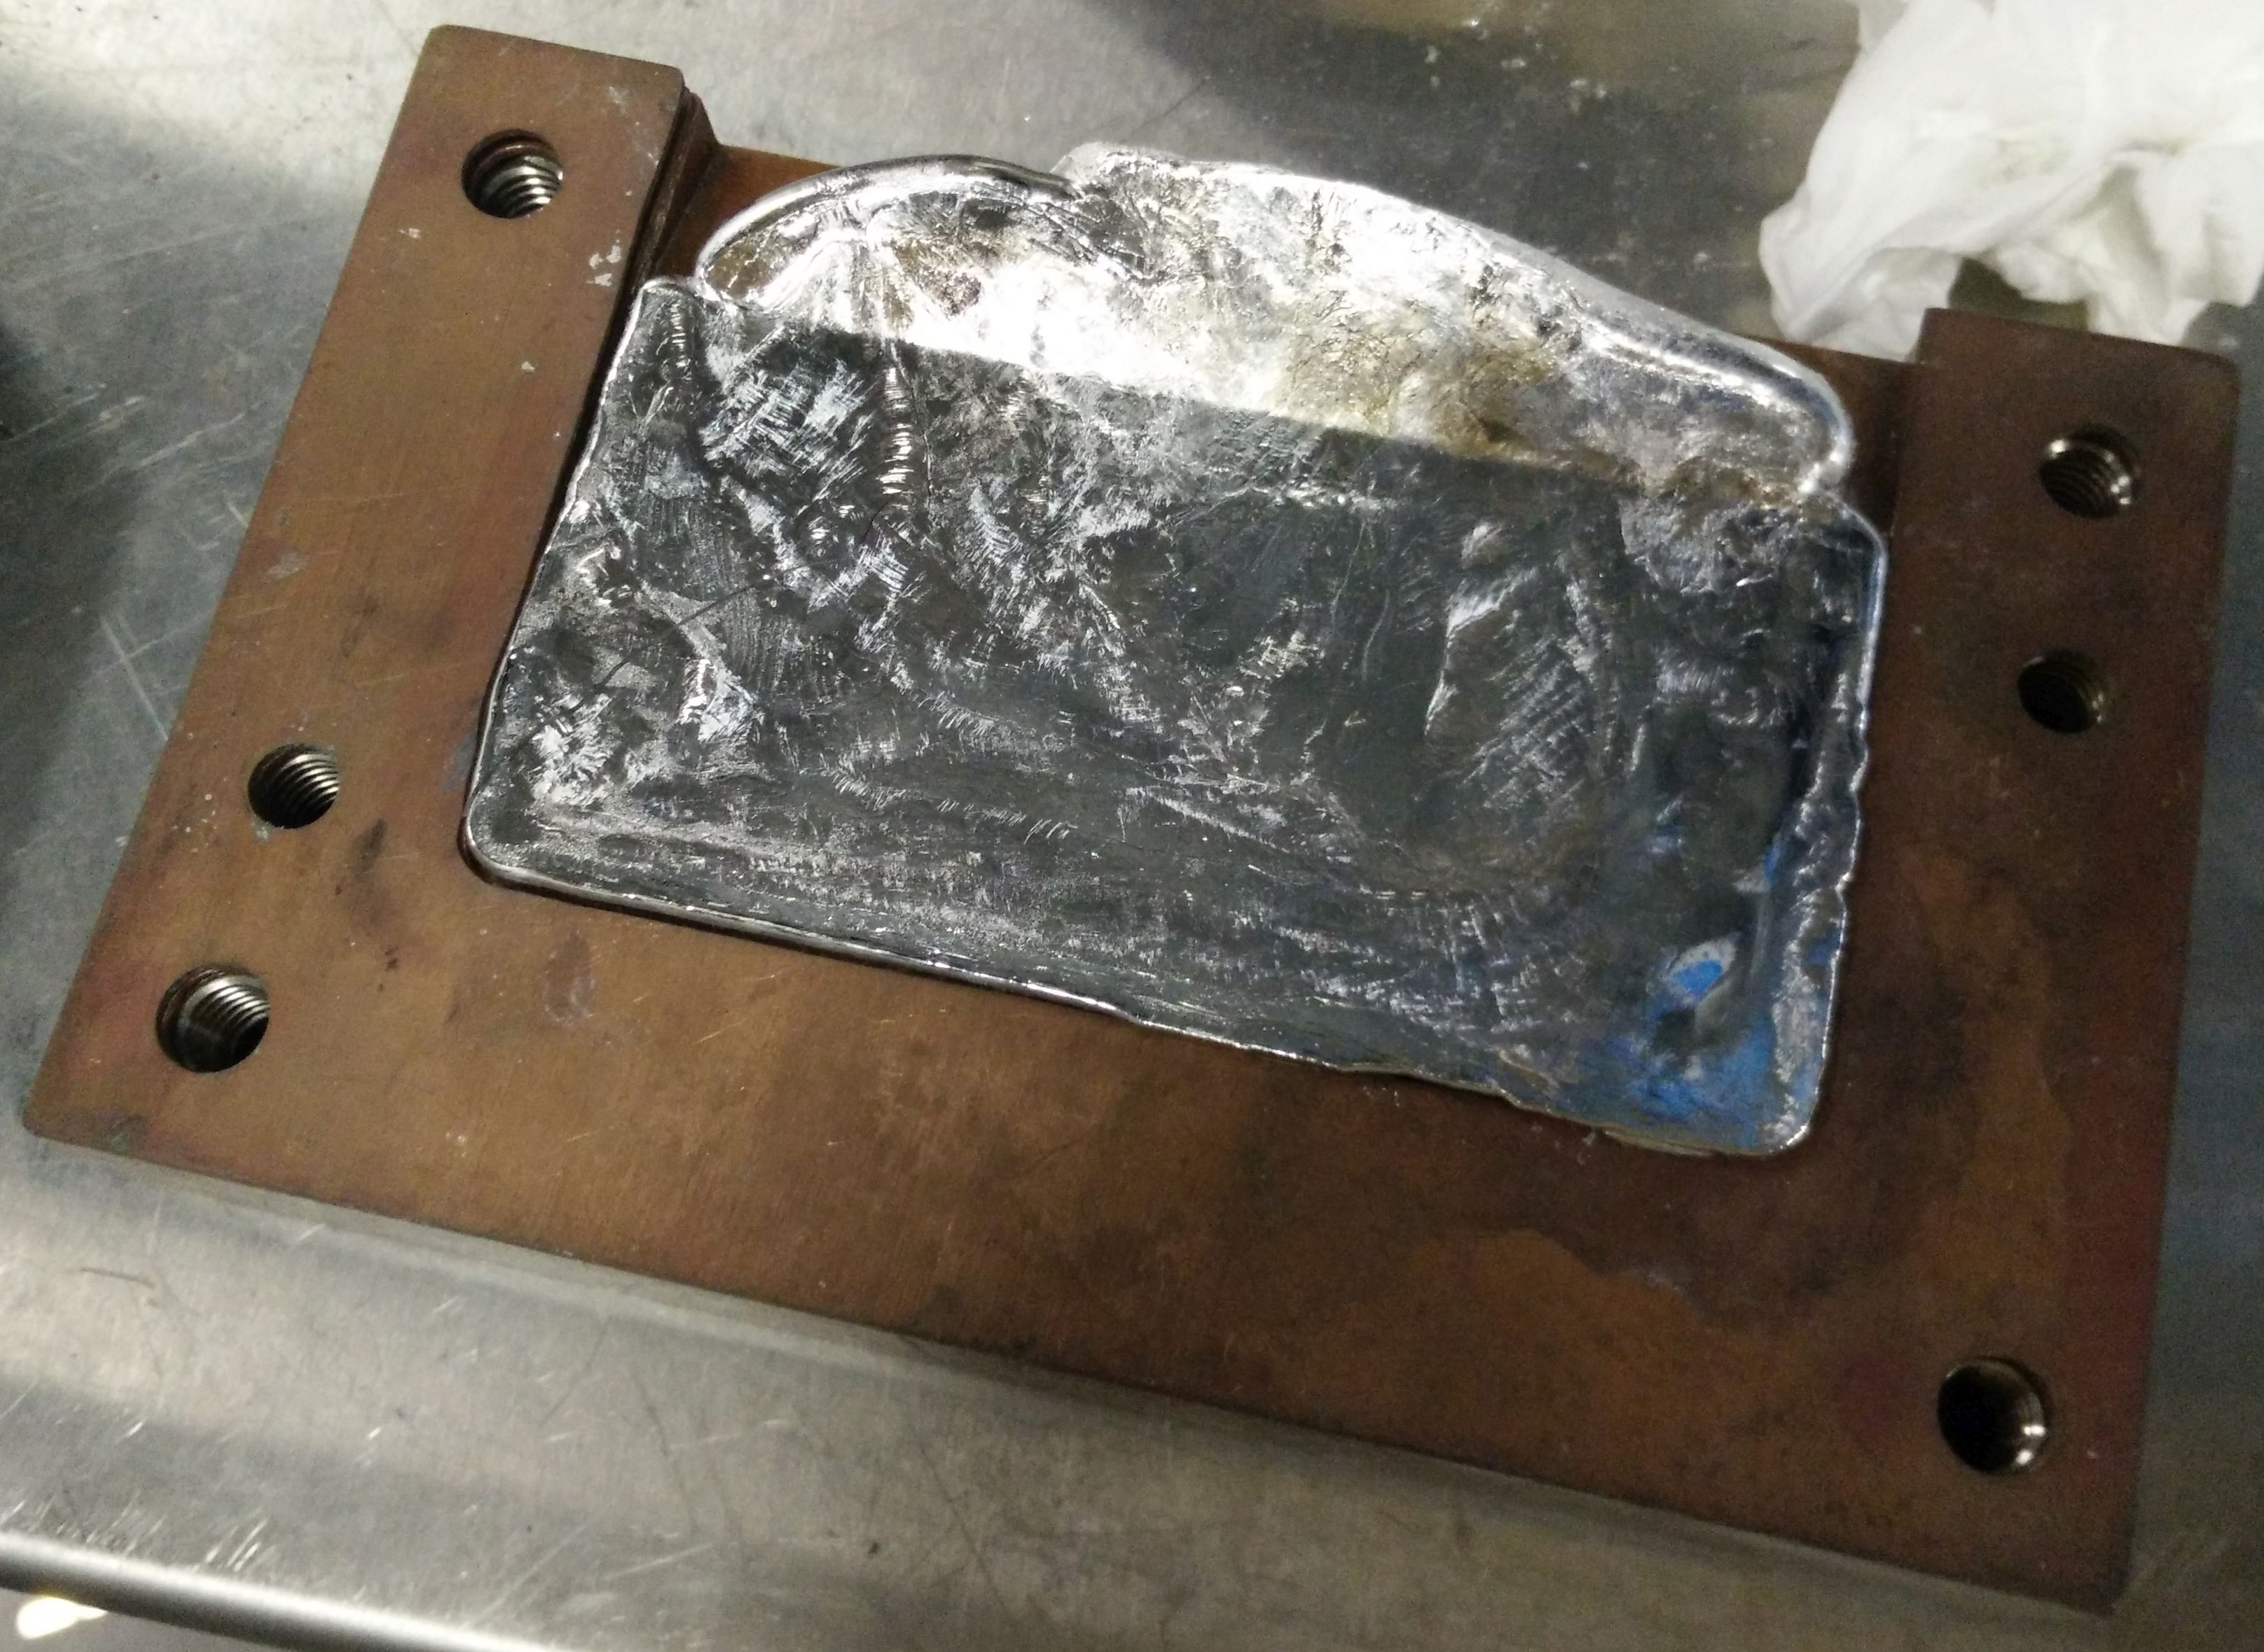
\includegraphics[width=\textwidth]{Ex_Mould_Cast_Plate.jpg}
		\caption{}
		\label{fig:FilledMould}
	\end{subfigure}
	\caption[(a) Inducting casting chamber. (b) Boron nitrate coated graphite crucible with Mg and Zn ingot charge. (c) 3D schematic of copper plate mould with dimentions. (d) Cast \MgZnCa~ master alloy plate within mould.]{(a) Inducting casting chamber. (b) Boron nitrate coated graphite crucible with Mg and Zn ingot charge. (c) 3D schematic of copper plate mould with dimentions. (d) Cast \MgZnCa~ master alloy plate within mould. (a) and (c) reproduced from \cite{Laws2007}.}%global caption
	\label{fig:Induction}
\end{figure}

\subsection{Final Shaping}
\subsubsection{Riser Removal} \label{sec:RiserRemoval}
Once master alloy plate was cast the riser was removed. The plate was mounted in a polymer grip vice and the riser carefully cut off with a 24 or 32 \acrshort{tpi} hacksaw. Paper was placed under the vice grips to capture the dust for later analysis (Figure \ref{fig:Vice}).

\subsubsection{Target Extraction}
The target was extracted from the plate by a notched $32~ mm$ diameter diamond bit drill on a Hercus Sales (W2) drill press at 360 \acrshort{rpm} with a bore rate of approximately $15~ mm/hr$. The plate was mounted in a polymer grip horizontal vice on top of cut plywood for dampening, and placed in a drip tray. A constant stream of lubricating distilled water was supplied by a standard spray bottle (Figures \ref{fig:DrillBit} and \ref{fig:DrillPress}).

\subsubsection{Target Rounding}
The target was then shaped to a nominally $1~ in$ ($25.2 - 25.4~ mm$) diameter disk by removal of excess circumferential material. Large sections were removed by hacksaw as outlined in Section \ref{sec:RiserRemoval}, with finer shaping accomplished by linishing operations. Target roundness was checked throughout by comparing with a 2 Euro or washer template, $25.75~ mm$ and nominal $1~ in$ diameter respectively. Final nominal target diameter was confirmed by vernier caliper measurement (Figure \ref{fig:TargetEuro}).  

\subsubsection{Target Polishing}
The target was progressively manually polished with light pressure on glass plate in a figure eight pattern with flowing lubricating water. Targets were polished on both sides and rotated through small angles every couple seconds to ensure a consistent flat surface. The grit progression was 320, 800, 1200, and 4000 with target washing between all stages. After 800 and higher grit stages the target was ultrasound cleaned for 1 minute in soap and water. Polishing wheels were not used because they produce a less consistent flat surface and targets require high surface tolerance to fire within the sputtering gun. Target flatness was checked by micrometre, with nominal variation between the two opposing surfaces being less than 1\% the target diameter, about $0.254~ mm$. 

%single image
\begin{figure}[htbp]
	\centering
	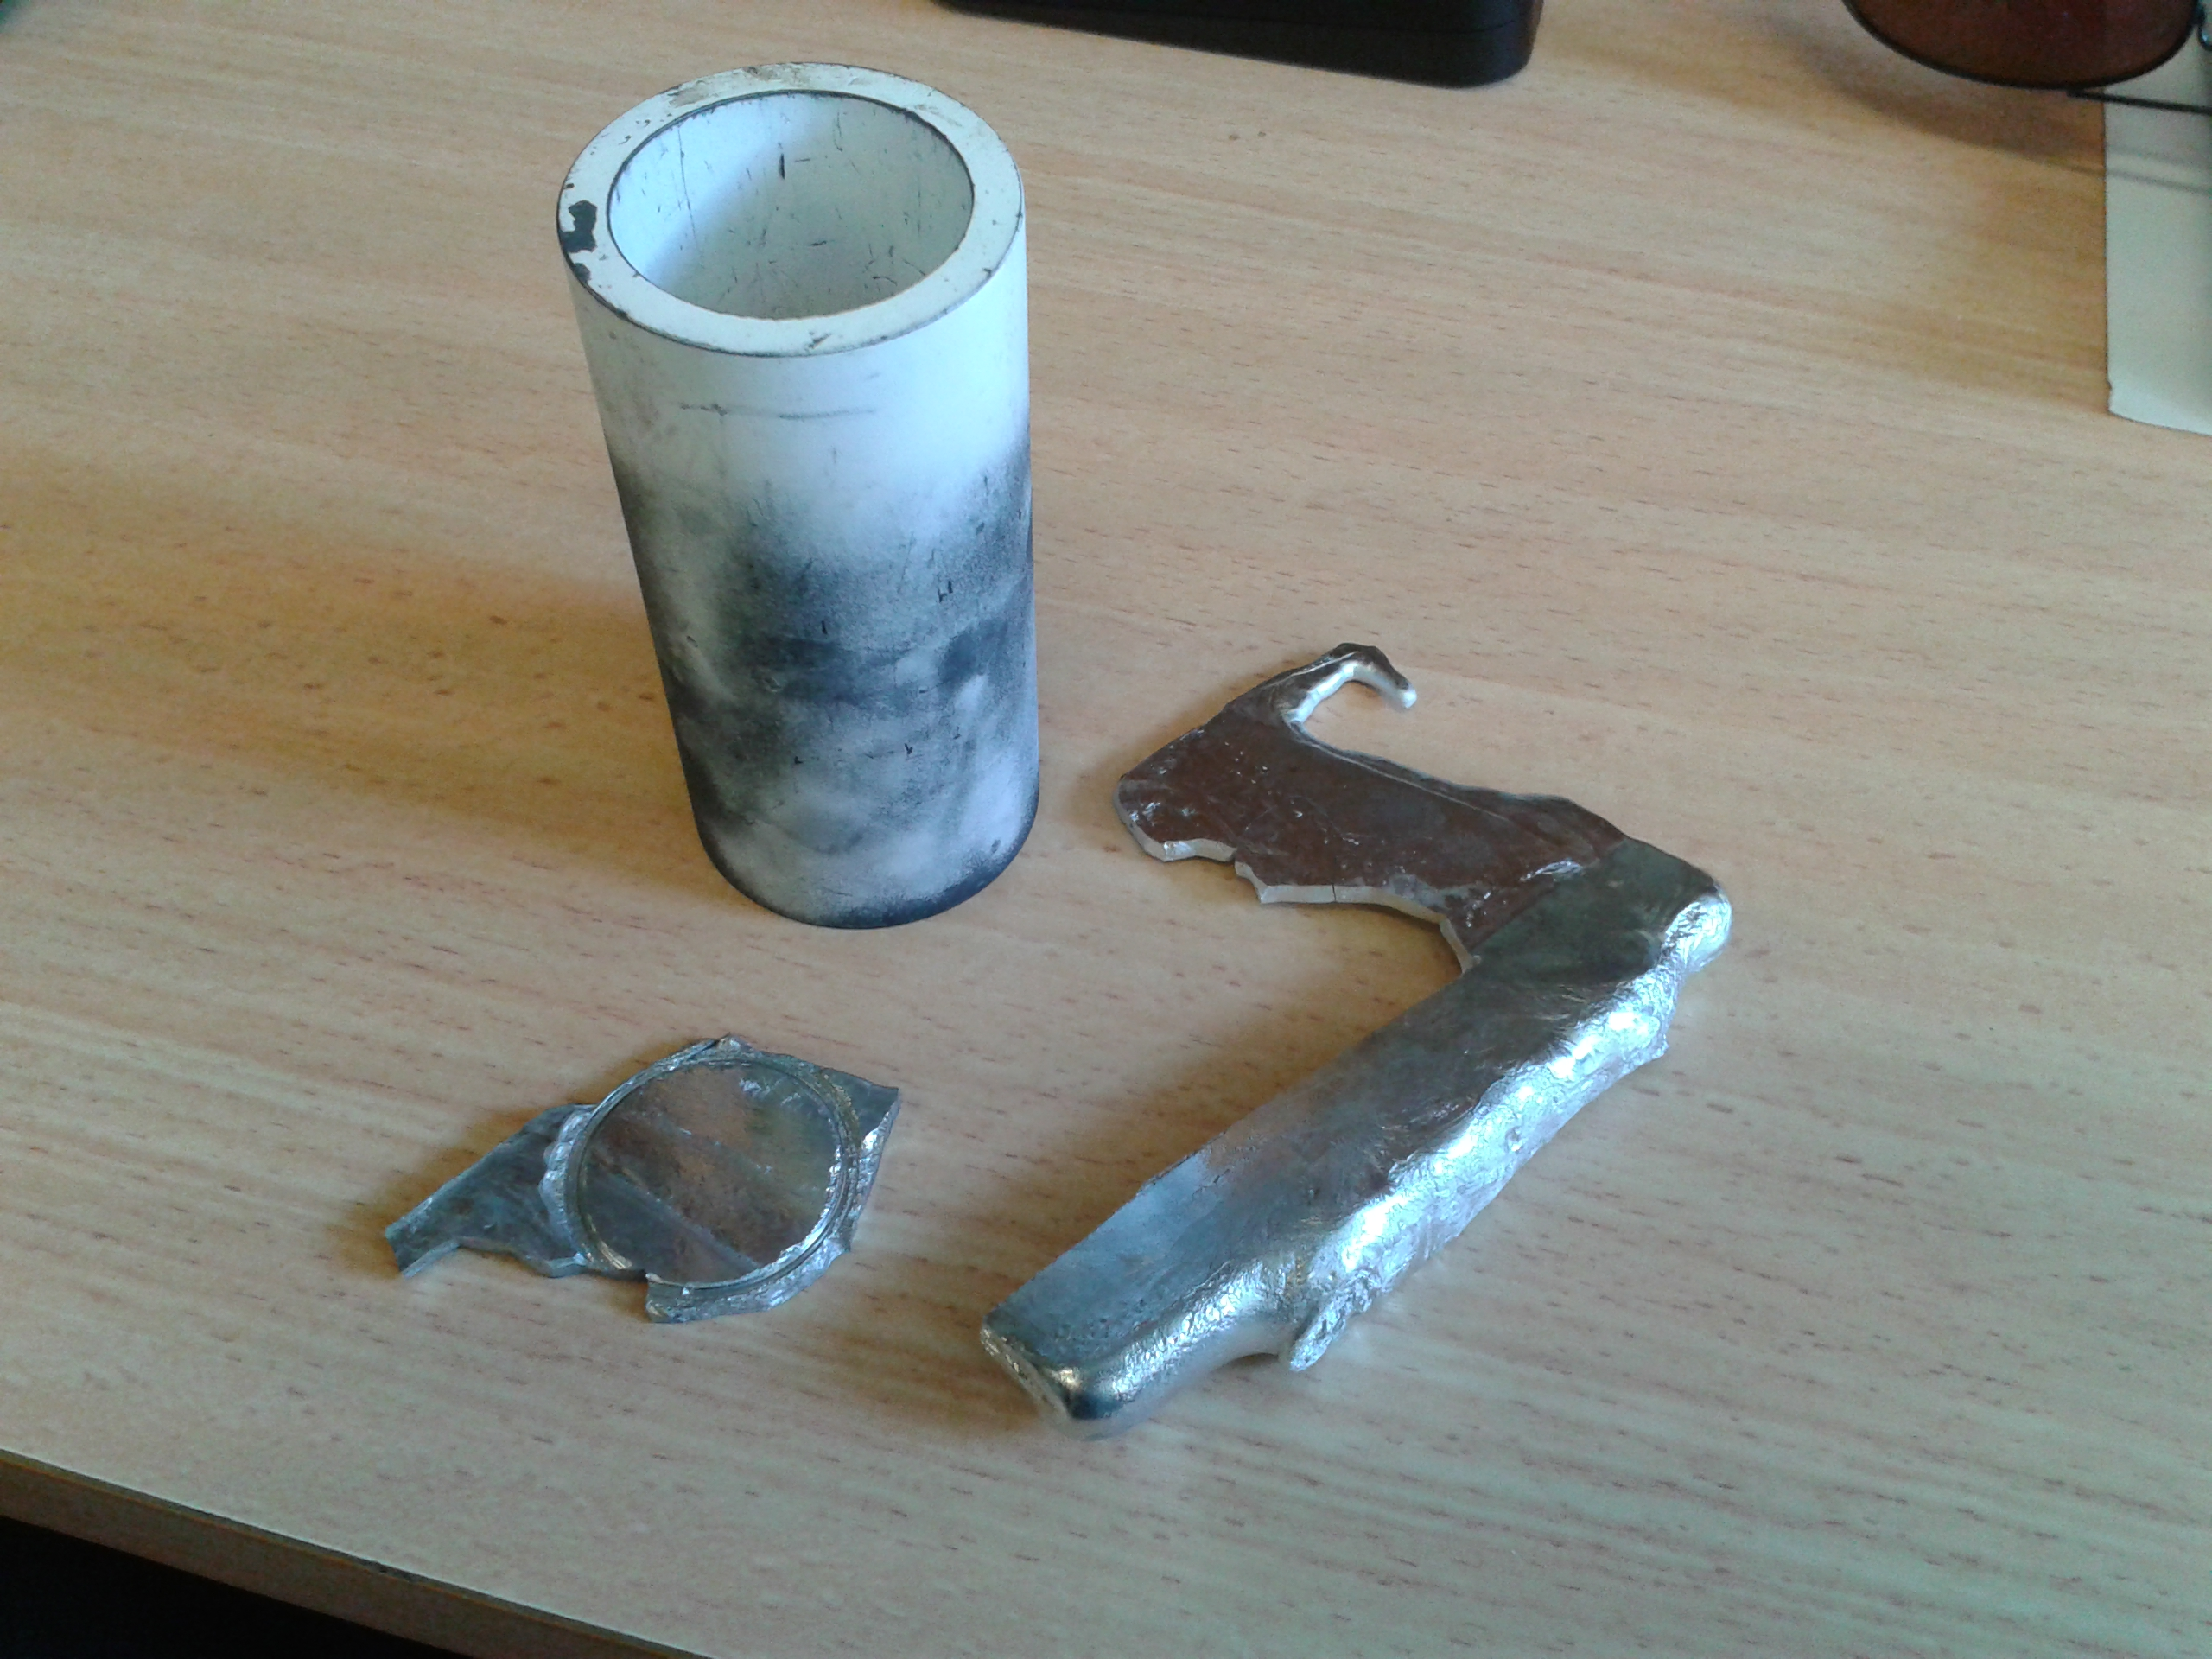
\includegraphics[width=0.75\textwidth]{Ex_CruciblePlateRiserRoughtarget.png}
	\caption{(a) Boron nitrate coated graphite crucible for induction furnace melting of alloys, (b) Cracked \MgZnCa~ master alloy plate, (c) Riser cut free from main casting, and (d) Drilled and partly shaped target.}
	\label{fig:CrucibleShaping}
\end{figure}

%code to put 4 images side by side in a figure
\begin{figure}[htbp]
	\centering
	%Image 1
	\begin{subfigure}[htbp]{0.49\textwidth}
		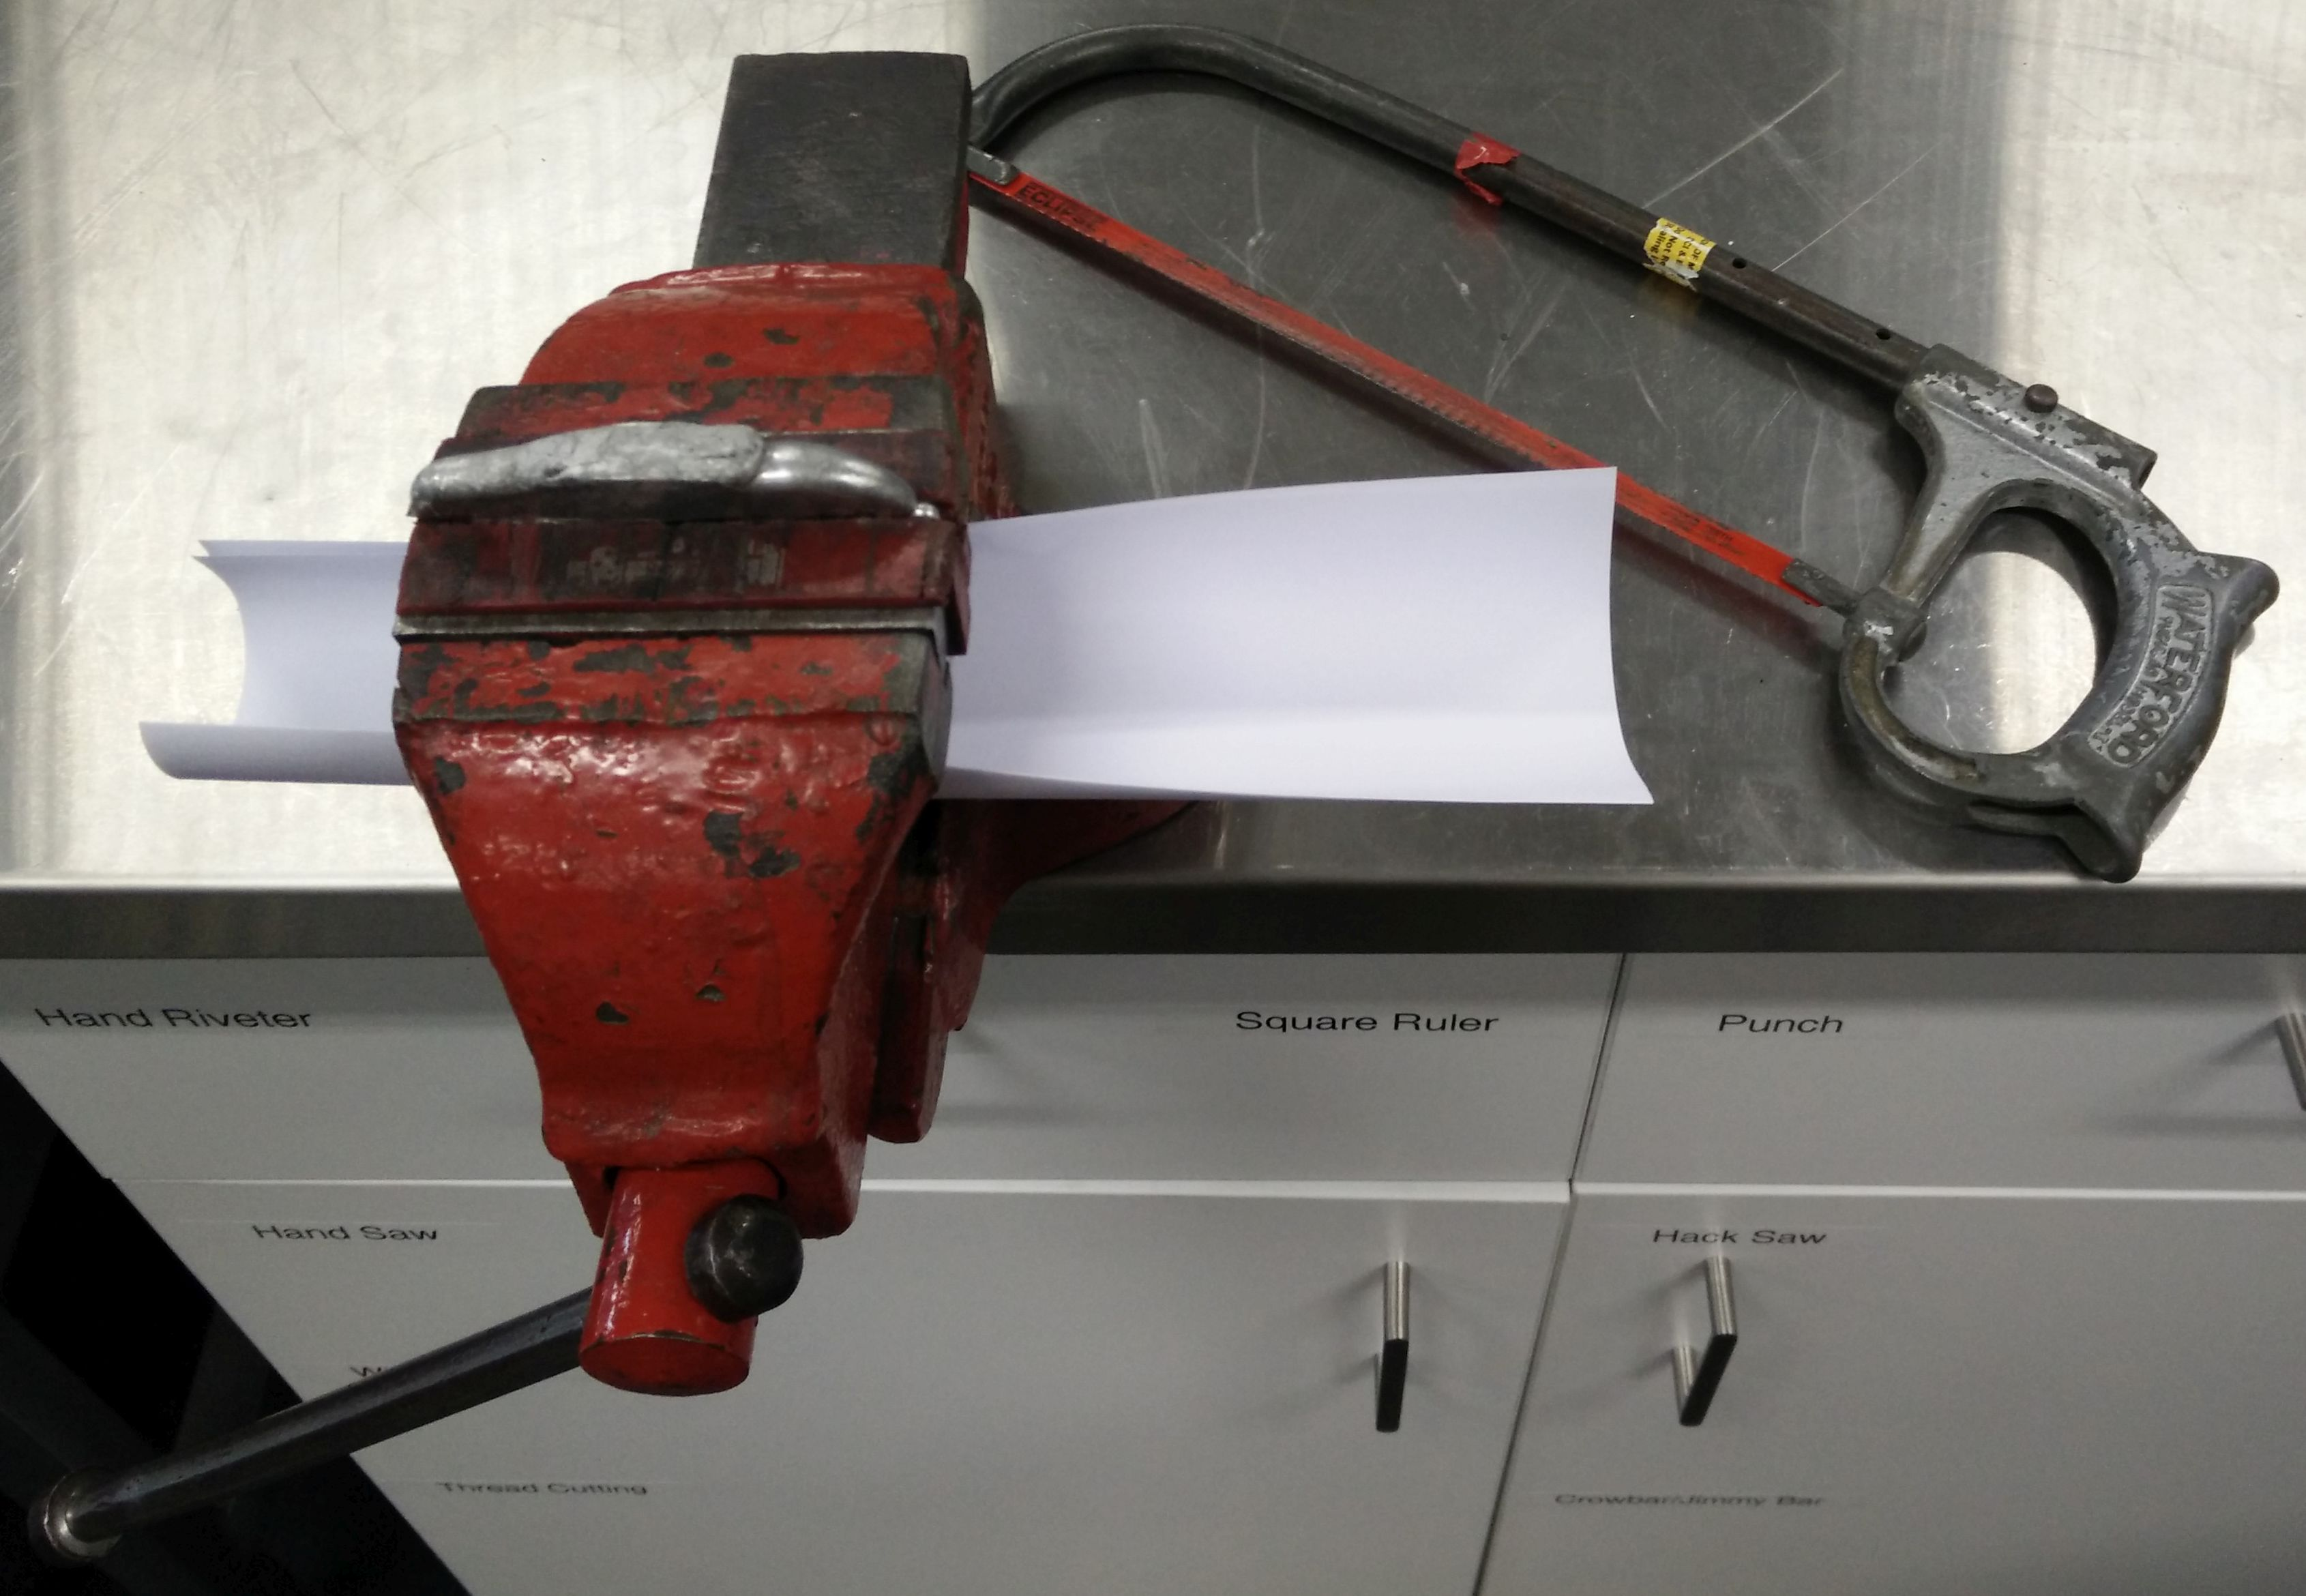
\includegraphics[width=\textwidth]{Ex_Vice_Hacksaw.jpg}
		\caption{}
		\label{fig:Vice}
	\end{subfigure}
	%Image 2
	\begin{subfigure}[htbp]{0.38\textwidth}
		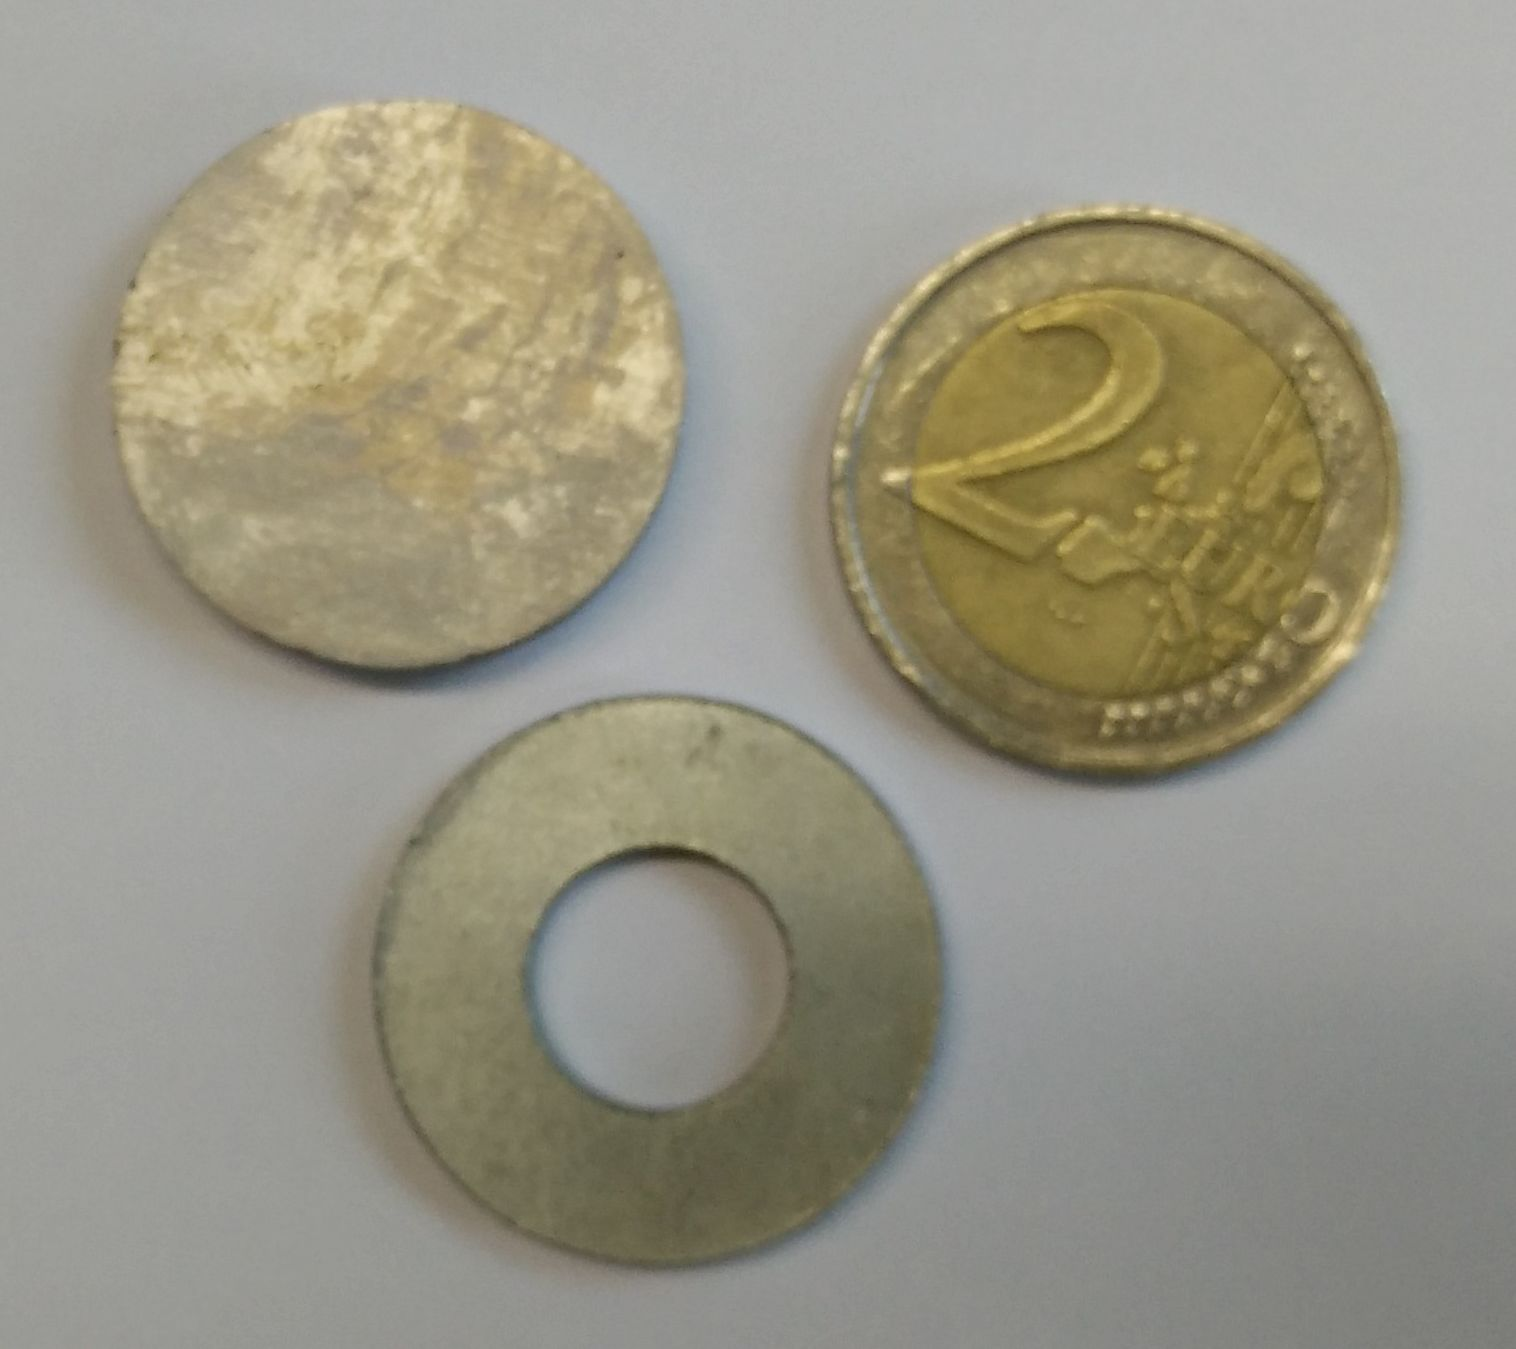
\includegraphics[width=\textwidth]{Ex_Target_Euro.jpg}
		\caption{}
		\label{fig:TargetEuro}
	\end{subfigure}
	%Image 3
	\begin{subfigure}[htbp]{0.275\textwidth}
		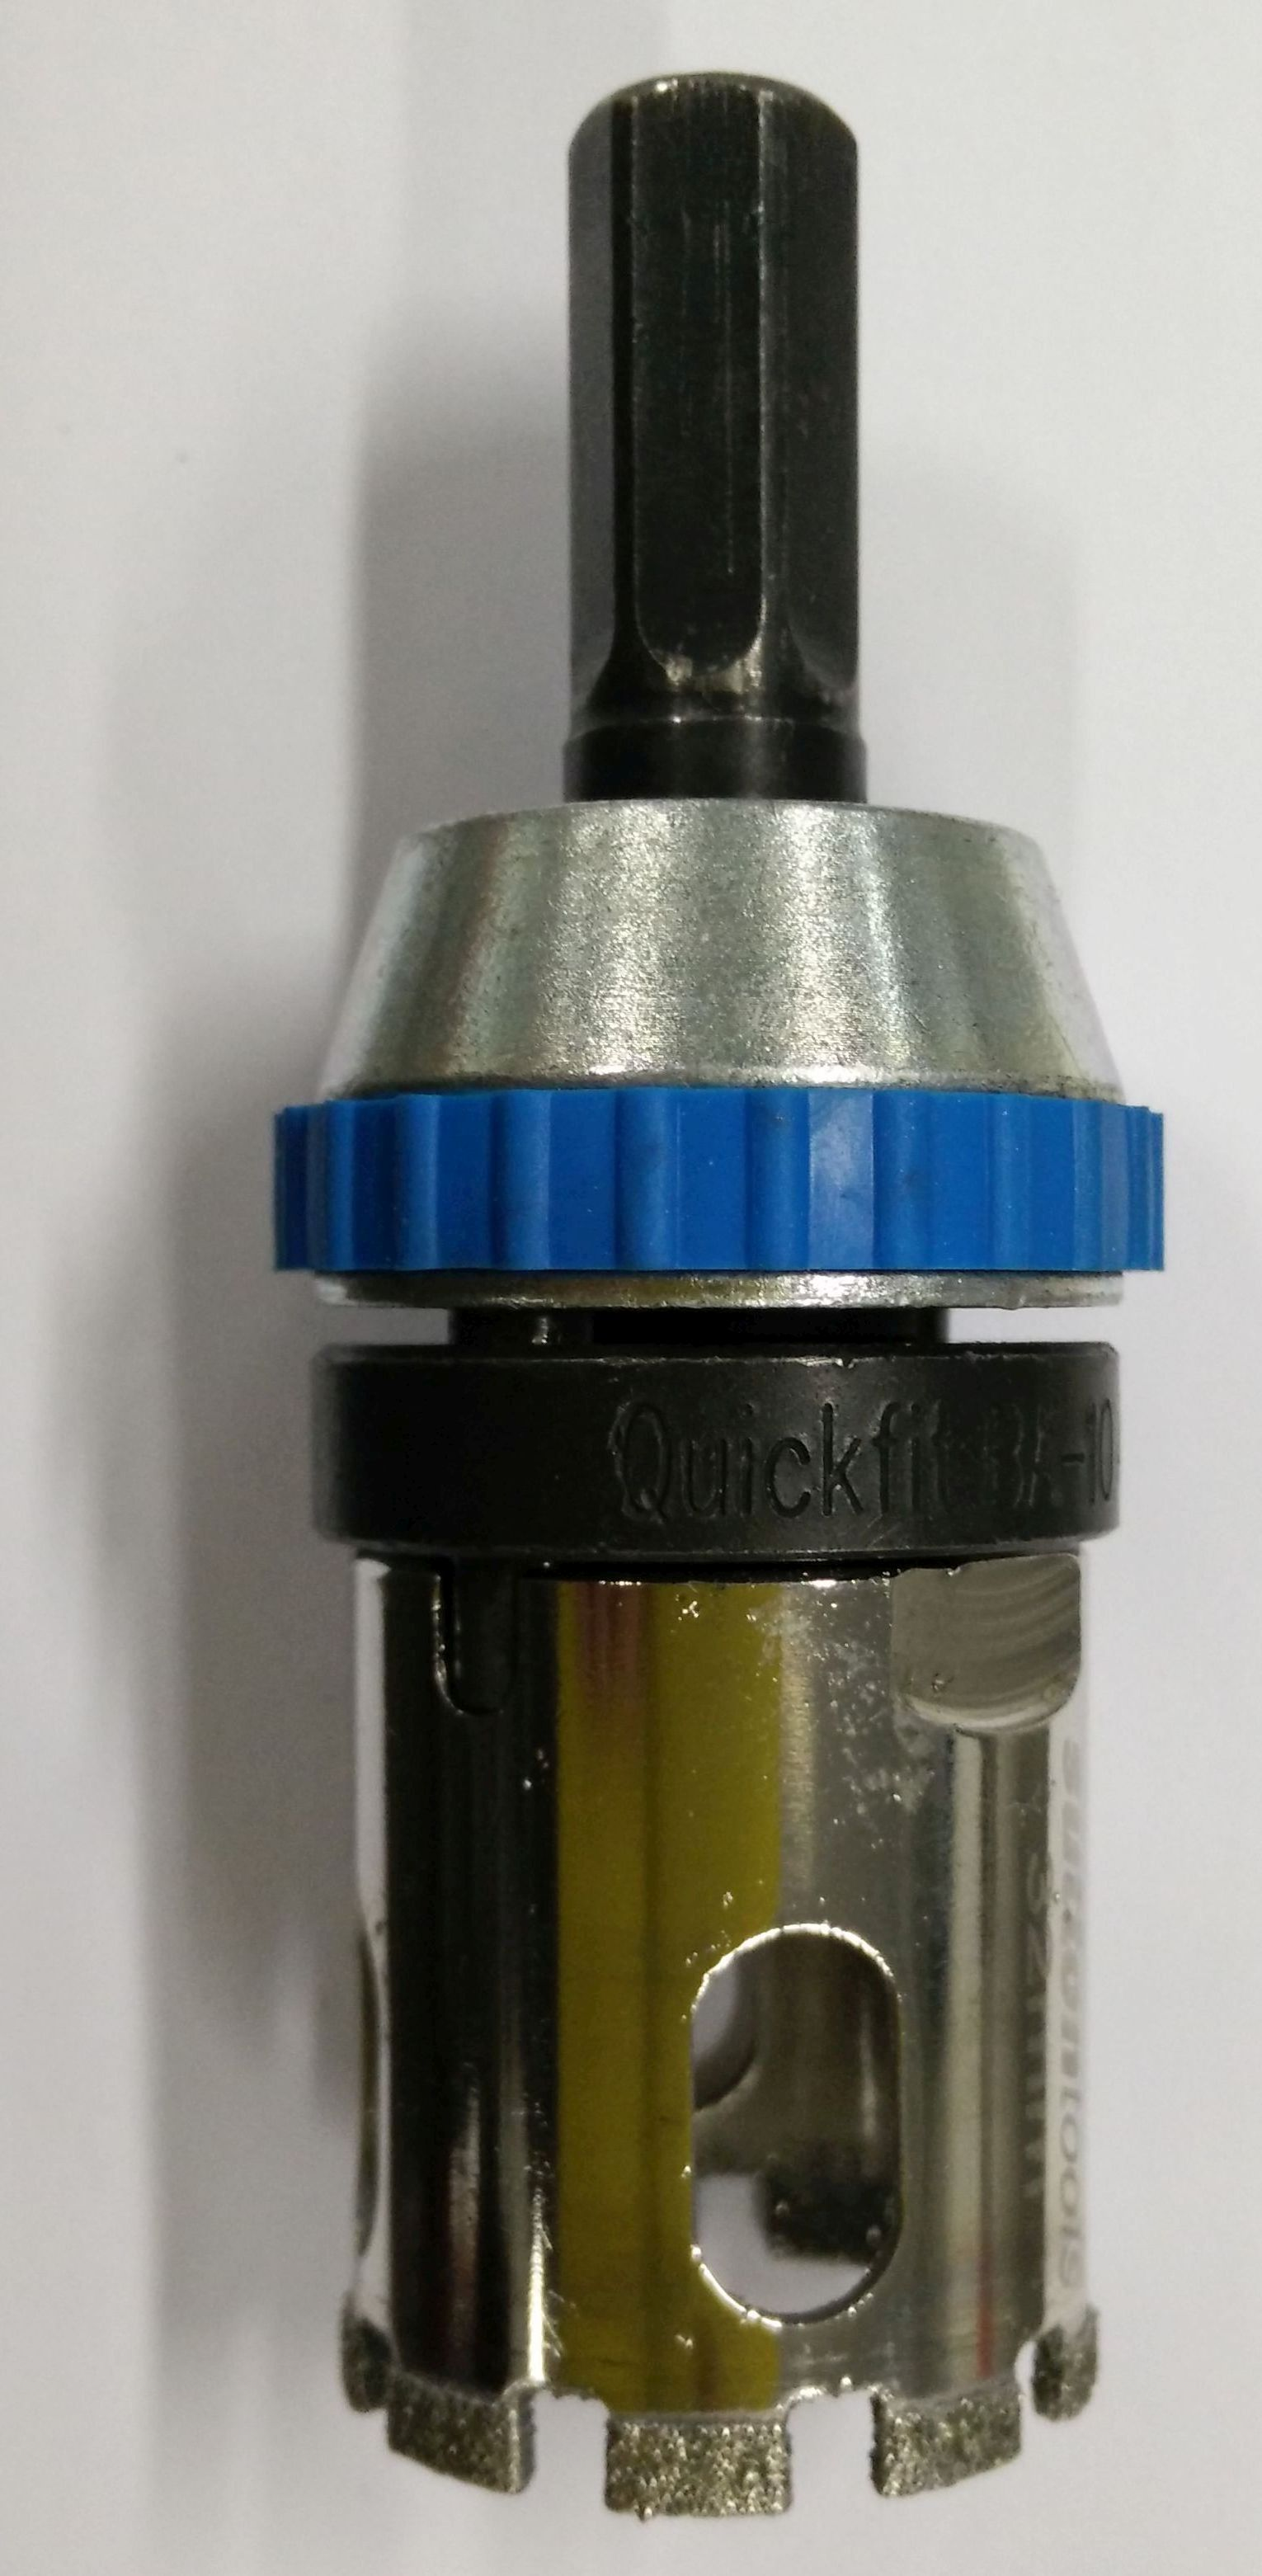
\includegraphics[width=\textwidth]{Ex_Drill_Bit.jpg}
		\caption{}
		\label{fig:DrillBit}
	\end{subfigure}
	%Image 4
	\begin{subfigure}[htbp]{0.30\textwidth}
		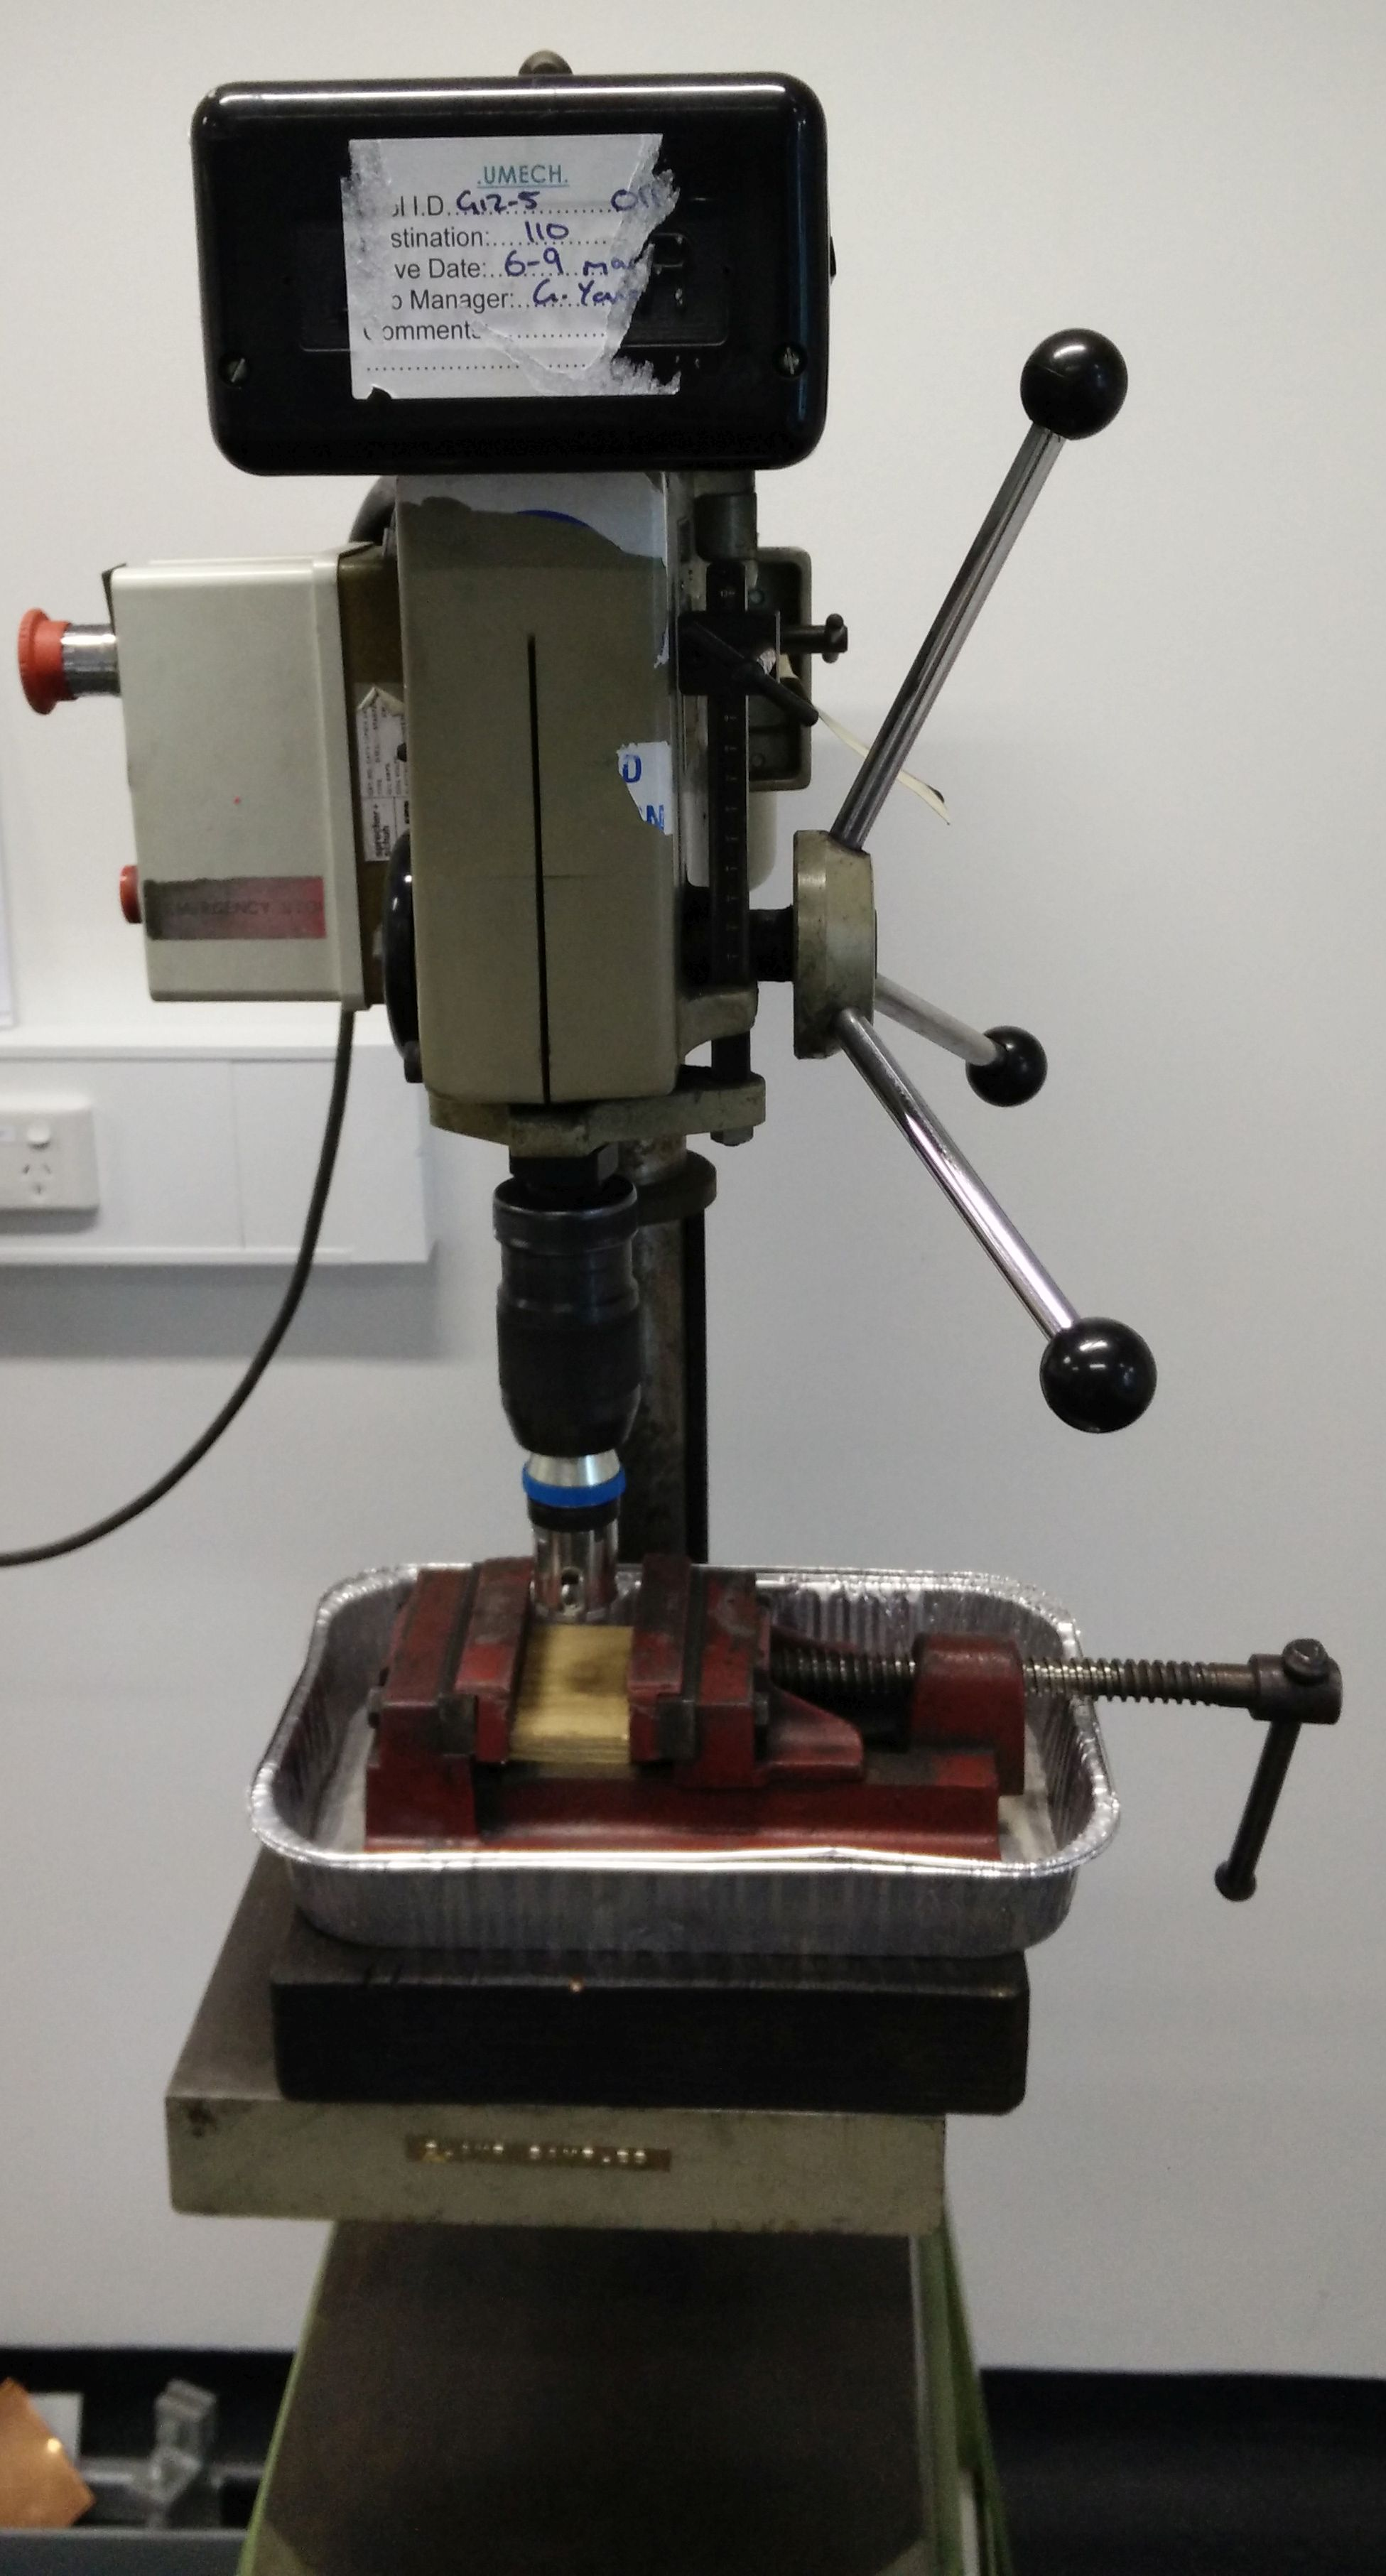
\includegraphics[width=\textwidth]{Ex_Drill_Press.jpg}
		\caption{}
		\label{fig:DrillPress}
	\end{subfigure}
	\caption{(a) Polymer grip vice clamping plate below riser with 32 \acrshort{tpi} hacksaw. (b) Fully shaped, unpolished target with 2 Euro and washer template. (c) Notched $32~ mm$ diameter diamond drill bit. (d) Drill press, bit, horizontial vice with polymer grips, plywood damper and drip tray for target extraction.}%global caption
	\label{fig:ShapingEquipment}
\end{figure}

\clearpage

\section{DC Magnetron Sputtering}
\subsection{DC Magnetron Sputtering Equipment}
The thin films were deposited by an in house \acrshort{dc} magnetron sputtering facility (Figure \ref{fig:CaoSputtering}). This facility has a maximum power of 50 W, with a working gas of ultra-high purity Ar (99.999\%). The sputtering gun nominal target diameter is $25.4~ mm$ ($1~ in$). The chamber can achieve a base vacuum pressure of at least $10^{-2}~ Pa$, and a working Ar pressure of at least $2~ Pa$ at constant flow rate of $2~ cm^{3}/s$. The chamber has direct access and a large deposition area, allowing for batch processing of multiple substrates simultaneously.

%single image
\begin{figure}[htbp]
	\centering
	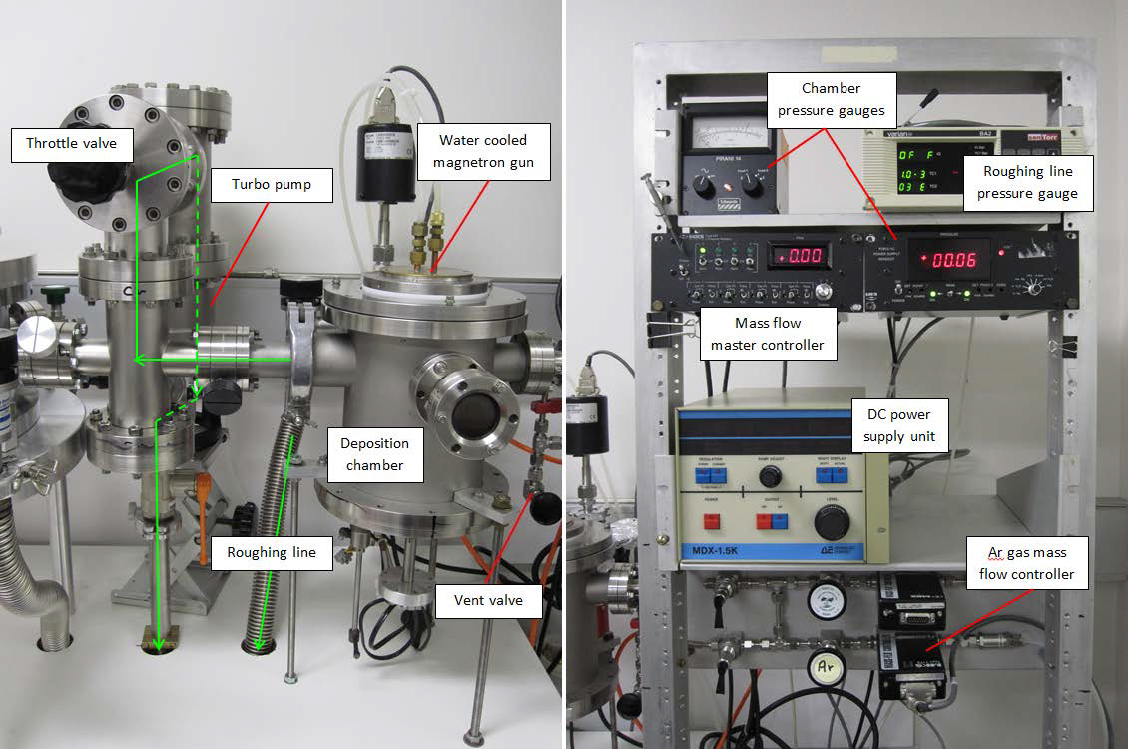
\includegraphics[width=0.75\textwidth]{Ex_Cao_SputterMachine.png}
	\caption[In house \acrshort{dc} magnetron sputtering facility.]{In house \acrshort{dc} magnetron sputtering facility. Reproduced from \cite{Cao2013}.}
	\label{fig:CaoSputtering}
\end{figure}

\subsection{Depostion of Thin Films}
A target was affixed in the sputtering gun mount by applying \hl{thermal gel} to one side for coincident contact. The desired substrate was position on the sample stage within the chamber and the chamber sealed. The chamber was evacuated to the desired base pressure, and then backfilled to the desired working Ar pressure. Coincident Ar pressure was maintained by a constant flow of Ar gas. This was necessary because the number of Ar$^{+}$ ions increases with chamber pressure, and accordantly increases the rate of deposition \cite{Ozeki2002}. Before deposition the targets were prepared by a pre-sputter to remove contamination and oxides from their surface. During this stage the substrates were protect by a shield positioned over the sample area preventing deposition.

The \glspl{tfmg} were deposited onto room temperature substrates, and \glspl{smg} onto elevated temperate substrates. The elevated substrate temperatures were achieved and controlled by a hot plate and K-type thermocouple.

The initial \gls{tfmg} sputtering parameters were based on Liu, et al. \cite{Liu2012} work on \ZrCuNiAl~ film refinement, and the \gls{smg} parameters were based on Yu, et al. \cite{Yu2013} and Aji, et al. \cite{Aji2013} work on \ZrCuAl~ and \ZrCuNiAl~ \gls{smg} films respectively. These parameters were refined by appropriate step sizes as required to suit the examined MgZnCa biocompatible systems. 

%table
\begin{table}[h]
	\centering
	\begin{tabular}{ l l l }
		\toprule
		Nominal Sputtering Parameters: & \acrshort{tfmg} & \acrshort{smg} \\
		\midrule
		Base Camber Pressure: & $3 \times 10^{-4} - 10^{-2}~ Pa$ & $5 \times 10^{-5} - 10^{-4}~ Pa$ \\
		Deposition Ar Pressure:	& $0.3 - 3.0~ Pa$ & $5\times 10^{-2} - 0.3~ Pa$\\
		Deposition Power Range:	& $30 - 50~ W$ & $30 - 50~ W$\\
		Max Deposition Rate: & $3.3~ nm s^{-1}$ & $1.4~ nm s^{-1}$ \\	 
		Substrate Deposition Temperature: & \acrshort{rt} & $0.7 - 0.8$ \acrshort{Tg} \\
		\bottomrule
	\end{tabular}
	\caption{Nominal Sputtering Parameters}
	\label{tab:NomSputterParameters}
\end{table} \todo{Probably will be much closer to the 50 W end (Jake topped out at 55 W).
MgCaZn has more light elements near Ar than ZrCuNiAl.
Therefore expect greater deposition efficiencies and to not require as much power.
ZrCuNiAl used 50 – 150 W, but we cannot get power that high unless we use 3 inch targets (not practical).} 	

\subsection{Target Lifespan}
Each target is expected to be able to deposit approximately $10 - 15~ \mu m$ of total film thickness onto a substrate, which is about an hour of deposition at rate of 3.3nm/s. After full deposition the targets are no longer usable and should be disposed. 

\section{Examined Substrates} 
The thin films will be deposited onto four different substrates for examination; silicon wafer, water soluble substrate, \gls{bmg} substrates, and \gls{pcl} scaffold substrates.

\subsection{Silicon Wafer Substrate}
Thin films are easily and readily deposed onto un-doped (100) silicon wafer with minimal difficult. This substrate allows film properties to be easily examined with minimal influence from the substrate (I.E. film amorphousness can be confirmed with confidence by \acrshort{xrd}). These substrates can be purchased. 

\subsection{Water Soluble Substrate} 
Depositing films onto water soluble substrates allows the films be physically separated from a substrate and examined without substrate influence. A possible candidate substrate is NaCl wafer which dissolve quickly with the application of water, allowing for the physical separation of the films. These substrates can be purchased. 

\subsection{BMG Substrate}
Depositing films onto \gls{bmg} substrates of similar composition allows for property modification effects of the films to be examined. Knowing the properties of the \gls{bmg} substrates and the applied films independently will allow the extent of the property modification to be fully evaluated, and should allow for modelling. These substrates can be manufactured as per the method described in Section \ref{sec:TargetManufacture}. \todo{Wedge mould to get amorphous metal!}

\subsection{Polycaprolactone (PCL) Scaffolds}
Depositing films onto \gls{pcl} scaffolds substrates will allow for examination of the films' effects and degradation performance. Ideally this will lead to the slow, controlled release of infused with antimicrobial, antibiotic, or analgesics packages.

\section{Thin Film Characterisation}
The properties of the \glspl{tfmg} and \glspl{smg} will be investigated by characterising the films after application to the different substrates; allowing standalone films as well as their substrate property modification effects to be investigated. 

\subsection{Physical and Chemical Properties}
The physical and chemical properties of the films will be characterised by a range of techniques; \acrshort{xrd}, \acrshort{dsc}, \acrshort{fib}, \acrshort{eds}, \acrshort{epma}, \acrshort{icp}, \acrshort{sem}, \acrshort{tem}, \acrshort{stem}, \acrshort{abed}, etc. 

\subsection{Quality of Deposition} 
The quality of the \gls{tfmg} deposition will be ascertained by investigation of the surface finish, coating adhesion, bonding, etc.

The rate of deposition will be calculated by dividing the measured film thickness (determined by \acrshort{tem}) by the total deposition elapse time. Thickness can also be measured by a 'stylus profiler.'

\subsection{Biocompatibility and Bioabsorption} 
The biocompatibility and bioabsorption of the \glspl{tfmg} will be characterised by cytotoxicity testing, \acrshort{pdp} scans, etc. 

%%%%%%%%%%%%%%%%%%%%%%%%%%%%%%%%%%%%%%%%%%%%%%%%%%%%%%%%%%%%%%%%%%%%%%%%%%

\chapter{RESULTS AND DISCUSSION}
\glsresetall

\section{Experimental Results} \todo{These are all for 3mm targets. Now using 4mm targets.}
\subsection{Casting Challenges and Observations}
When casting the target plates it was found slow melt pouring resulted in a poor mould fill while quicker pour experienced greater fills. The thin plate and relatively large mould riser creates a notable cooling difference between the two sections within the casting. It is believe this temperature gradient encourages the formation of cracks which often make the casting unusable. Additionally, the casting often display porosity within the plate, which may result in increased brittleness of the material. 

Once the casting size was increased from 3mm thickness to 4mm the fill problems and thermal cracking were largely mitigated. These 4mm plates often experience full or near full fills, and displayed much less cracking. The 4mm plates appear to have fewer internal defects as it has been possible to extract two nominal targets from each plate, while was difficult to extract even one target from the 3mm plate. 

\subsection{DSC Scans}
Isochoric \gls{dsc} scans are performed as a simple check for amorphous alloy structure by looking for evidence of the distinct exothermal \gls{Tg} and \gls{Tx} recrystallization peaks, and the endodermal \gls{Tm} and \gls{Tl} troughs. Scans are performed at heating rate of 20K/min in sealed alumina crucibles under a protective Ar atmosphere.

\subsection{Target Structure}
Ideal \MgZnCa~ targets should be completely amorphous as this should make them more resistance to corrosion before use, and provide a more homogenous distribution of constructional elements within the targets. The initial \gls{dsc} scans of the targets produced thus far do not display clear exothermal peaks, indicating they are not fully amorphous. However it is possible the targets are semi-crystalline, especially given how subtle exothermal peaks can be in MgZnCa systems \cite{Gu2010}. 

It is expected \gls{xrd} analysis may be able to provide more detail into the structure of the target plates as this technique has proven effective in differentiating between amorphous, semi-crystalline, and crystalline MgZnCa alloy \cite{Schluter2012, Wang2012}, although it can still be difficult \cite{Zhou2013}. Fully amorphous MgZnCa should display wide halo peaks around 38\degree and 66\degree (2 theta) and no additional sharp peaks, while semi-crystalline alloy would start to displace additional peaks \cite{Cao2013b, Gu2005, Wang2012, Gu2010, Cao2012}. 

Alloys of similar composition, like Mg$_{70}$Zn$_{25}$Ca$_{5}$, have a low \gls{gfa} with a \gls{tmax} of only about 3mm \cite{Gu2005, Zhou2013}. This coupled with the casting riser's (Figure \ref{fig:CrucibleShaping}c) ability to hold heat and thus extend the solidification time provides evidence that some amount of crystallization should be expected within the plate casting. 

The work of Schlüter, et al. \cite{Schluter2012}, Zhou, et al. \cite{Zhou2013}, and Wang, et al. \cite{Wang2012} on Mg$_{60}$Zn$_{35}$Ca$_{5}$, Mg$_{70}$Zn$_{25}$Ca$_{5}$, and Mg$_{67}$Zn$_{28}$Ca$_{5}$ respectively shows, semi-crystalline structures display both lower corrosion current density and more noble corrosion potential in comparison to fully crystalline alloy, and similar values to amorphous alloy. Hence semi-crystalline targets are expected to be relativity stable from crystalline galvanic/intergranular corrosion between the alloy constituents. 

%single image
\begin{figure}[htbp]
	\centering
	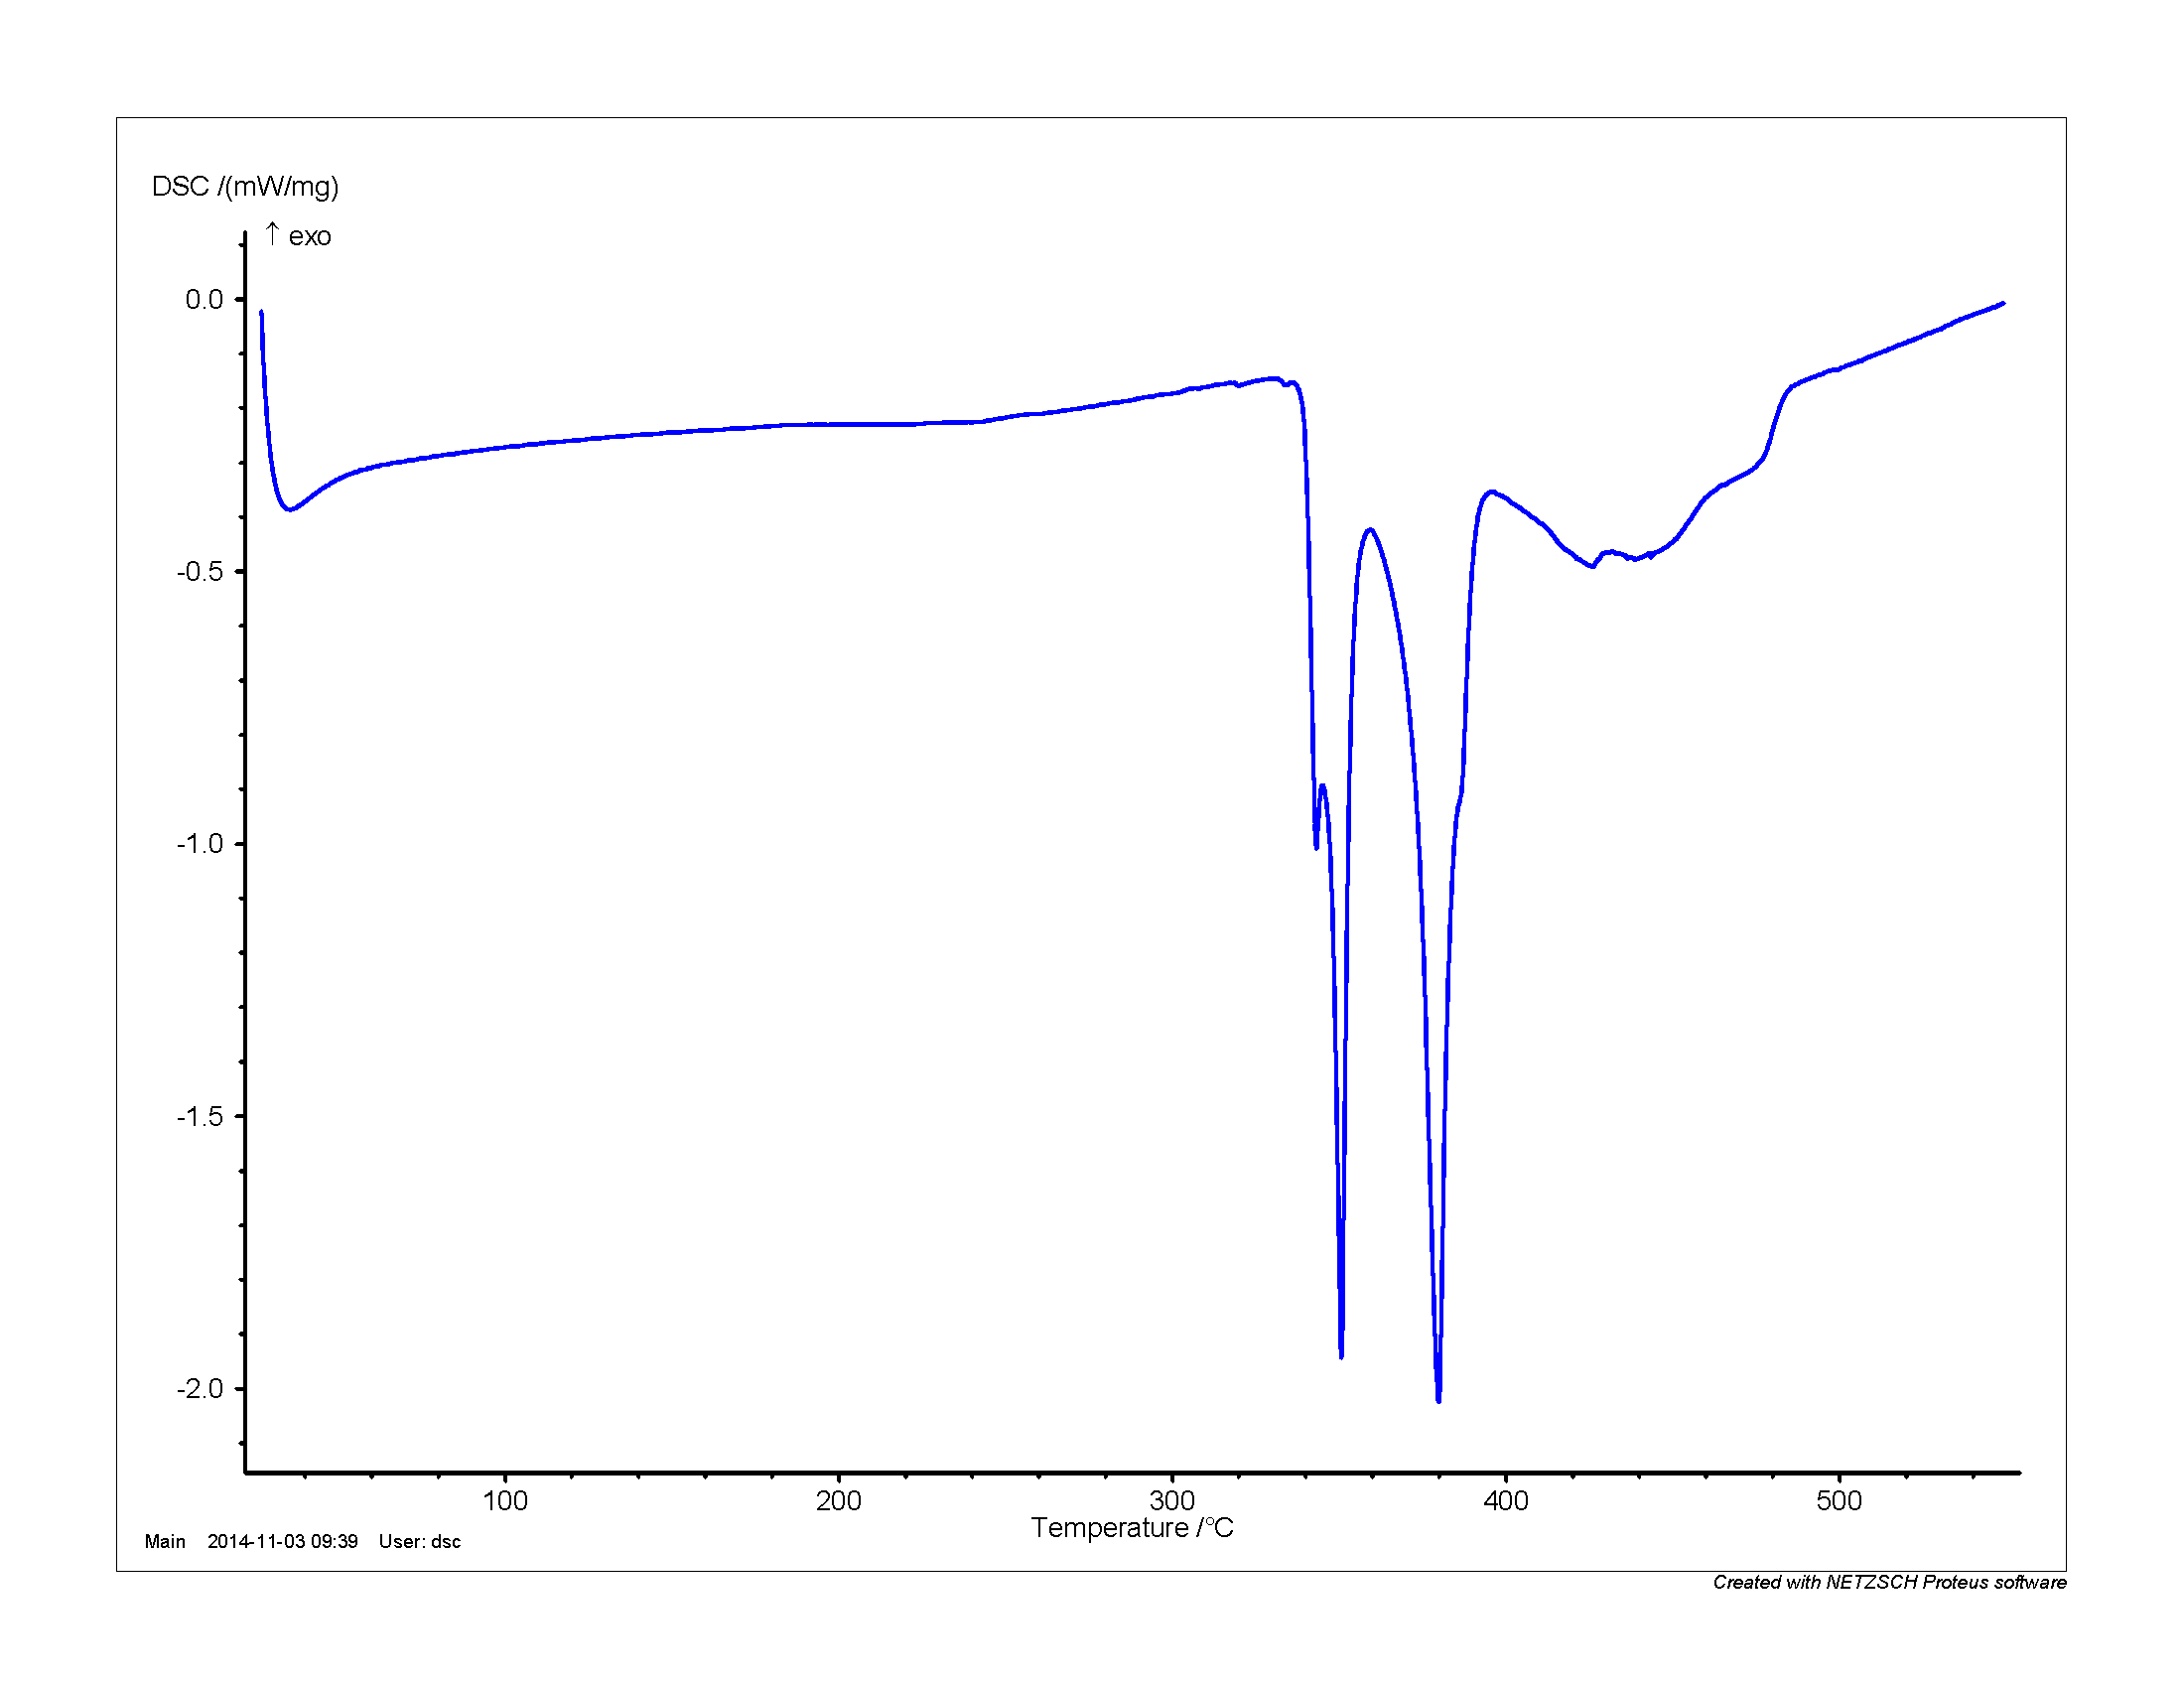
\includegraphics[width=0.75\textwidth]{T1_Curve2_Test2+Correction_20kmin_MgZnCa_301014.png}
	\caption{\acrshort{dsc} trace of the 3mm \MgZnCa~ target plate casting. The trace shows clear endothermic troughs indicating \acrshort{Tm} and \acrshort{Tl}, but no clear exothermal peaks which would indicate \acrshort{Tg} and \acrshort{Tx}. This data suggest the casting is primary crystalline.}
	\label{fig:DSCTarget1}
\end{figure}

However Zhou, et al. \cite{Zhou2013} has shown that despite this amorphous alloy has increased cathodic reaction kinetics and decreased anodic reaction when compared to \acrshort{comp} Mg, suggesting the corrosion rate of amorphous and semi-crystalline alloys is not significantly different from pure Mg. 

Ehrler \cite{Ehrler2008} master's on amorphous ribbons found Mg$_{67}$Zn$_{28}$Ca$_{5}$ becomes more brittle after 4 days of aging at \gls{rt}. Suggest targets should be shaped as soon as possible after casting in order to maximise ductility. 

\subsection{Target Composition}

\Acrshort{icp} testing found the first 3mm target plate only has about 26\% Zn. This is a loss of about 13\% Zn, or 8 grams of the total 108 grams of alloy cast. \todo{Draft result. And rough numbers. Put in correct ones if you use this.} This is too much material to attribute to loses, implying the Zn has migrated to riser during cooling. Injection moulding may produce more even cooling and better composition. 

\Gls{eds} analysis by \gls{sem} (S3400 Hitachi) on the first five plates has shown (insert results here). 

%%%%%%%%%%%%%%%%%%%%%%%%%%%%%%%%%%%%%%%%%%%%%%%%%%%%%%%%%%%%%%%%%%%%%%%%%%

\chapter{SUMMARY AND CONCLUSIONS}
\glsresetall

Found \glspl{tfmg} and \glspl{smg} were...

This implies...

Significant because...


%%%%%%%%%%%%%%%%%%%%%%%%%%%%%%%%%%%%%%%%%%%%%%%%%%%%%%%%%%%%%%%%%%%%%%%%%%

%Bibliography
\bibliography{ThesisBib}
\bibliographystyle{unsrt}

%%%%%%%%%%%%%%%%%%%%%%%%%%%%%%%%%%%%%%%%%%%%%%%%%%%%%%%%%%%%%%%%%%%%%%%%%%

\chapter{APPENDICES}

\section{MgZnCa Binary Phases}

%single image
\begin{figure}[h]
	\centering
	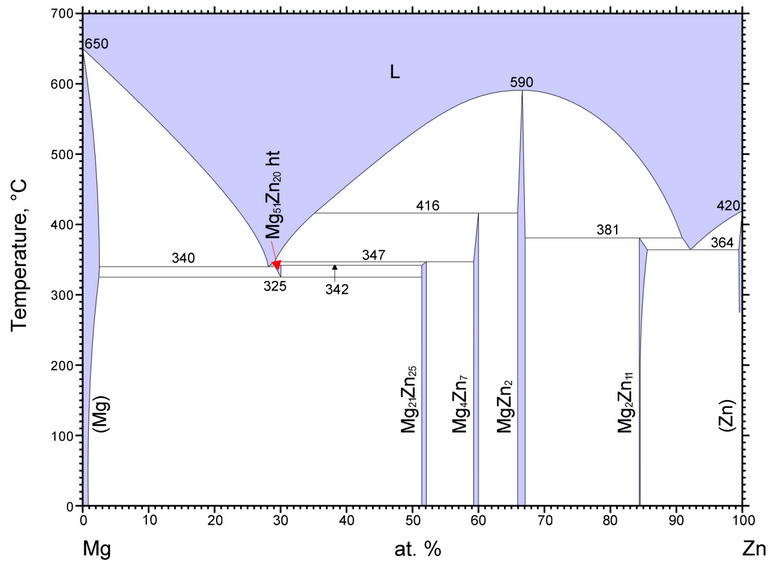
\includegraphics[width=0.9\textwidth]{Ph_Mg-Zn_Binary_Phase_Diagram.png}
	\caption[Mg-Zn binary phase diagram.]{Mg-Zn binary phase diagram. Reproduced from \cite{Predel1997}.}
	\label{fig:MgZnDiagram}
\end{figure}

%single image
\begin{figure}[h]
	\centering
	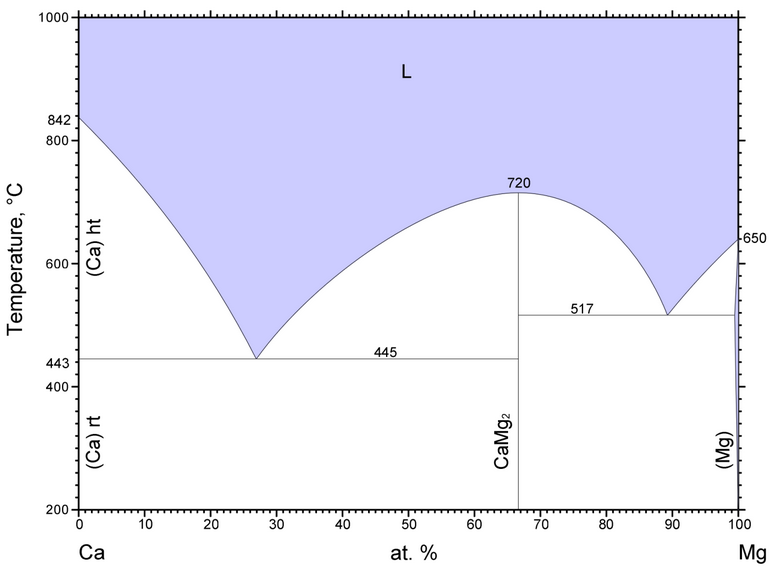
\includegraphics[width=0.9\textwidth]{Ph_Ca-Mg_Binary_Phase_Diagram.png}
	\caption[Ca-Mg binary phase diagram.]{Ca-Mg binary phase diagram. Reproduced from \cite{Nayeb1987}.}
	\label{fig:CaMgDiagram}
\end{figure}

%single image
\begin{figure}[h]
	\centering
	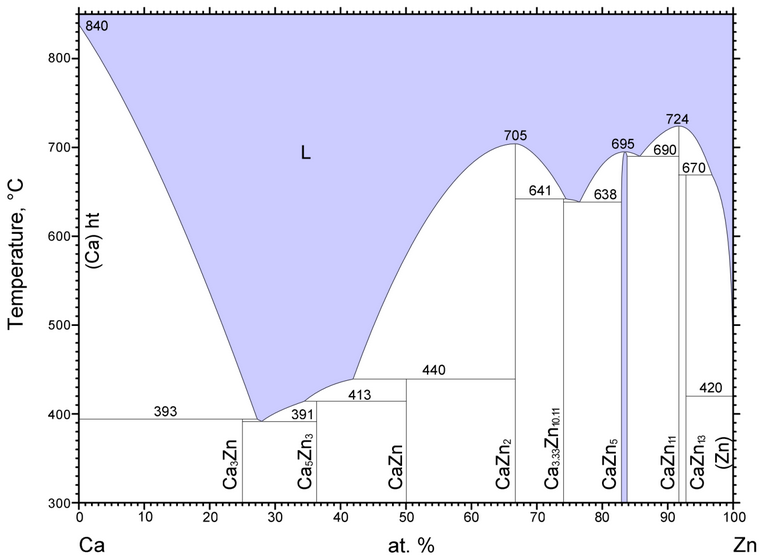
\includegraphics[width=0.9\textwidth]{Ph_Ca-Zn_Binary_Phase_Diagram.png}
	\caption[Ca-Zn binary phase diagram.]{Ca-Zn binary phase diagram. Reproduced from \cite{Itkin1990}.}
	\label{fig:CaZnDiagram}
\end{figure}

\clearpage
\newpage

\section{MgZnCa Ternary Phases}

%single image
\begin{figure}[htb]
	\centering
	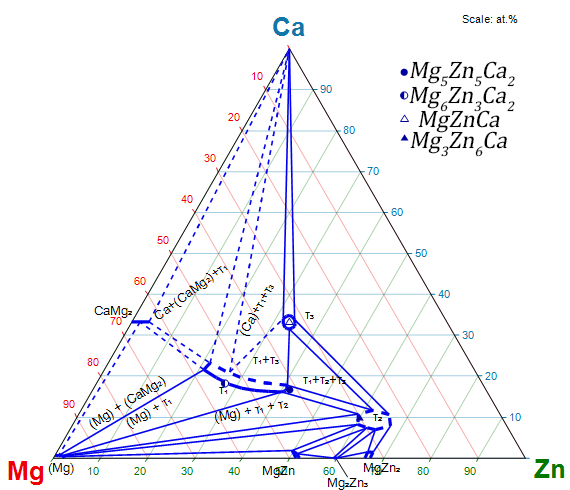
\includegraphics[width=0.9\textwidth]{Ph_MgZnCa300CPhaseDiagram_SprMats.png}
	\caption[Mg-Zn-Ca ternary phase diagram; partial isothermal at 300\degree C.]{Mg-Zn-Ca ternary phase diagram; partial isothermal at 300\degree C. Modified from \cite{Melnik1978}.}
	\label{fig:MgZnCa300PhaseD}
\end{figure}

%table
\begin{table}[H]
	\centering
	\begin{tabular}{ l l l }
		\toprule
		Phase & Composition & Source \\
		\midrule
		$T_{1}$ & Mg$_{6}$Zn$_{3}$Ca$_{2}$ OR & \cite{Clark1961} \\
		& Mg$_{5}$Zn$_{5}$Ca$_{2}$ & \\
		$T_{2}$	& Mg$_{5}$Zn$_{13}$Ca$_{2}$ OR & \cite{Clark1961} \\
		& Mg$_{3}$Zn$_{6}$Ca & \\
		$T_{3}$	& MgZnCa & \cite{Schulze1961} \\
		\bottomrule
	\end{tabular}
	\caption[Mg-Zn-Ca ternary phases $T_{1}$, $T_{2}$, and $T_{3}$ of Figure \ref{fig:MgZnCa300PhaseD}. Note: The first composition of both $T_{1}$ and $T_{2}$ are better supported by data.]{Mg-Zn-Ca ternary phases $T_{1}$, $T_{2}$, and $T_{3}$ of Figure \ref{fig:MgZnCa300PhaseD}. Note: The first composition of both $T_{1}$ and $T_{2}$ are better supported by data. Compiled from \cite{Clark1961, Schulze1961}.}
	\label{tab:SputterParameters}
\end{table}

%single image
\begin{figure}[htb]
	\centering
	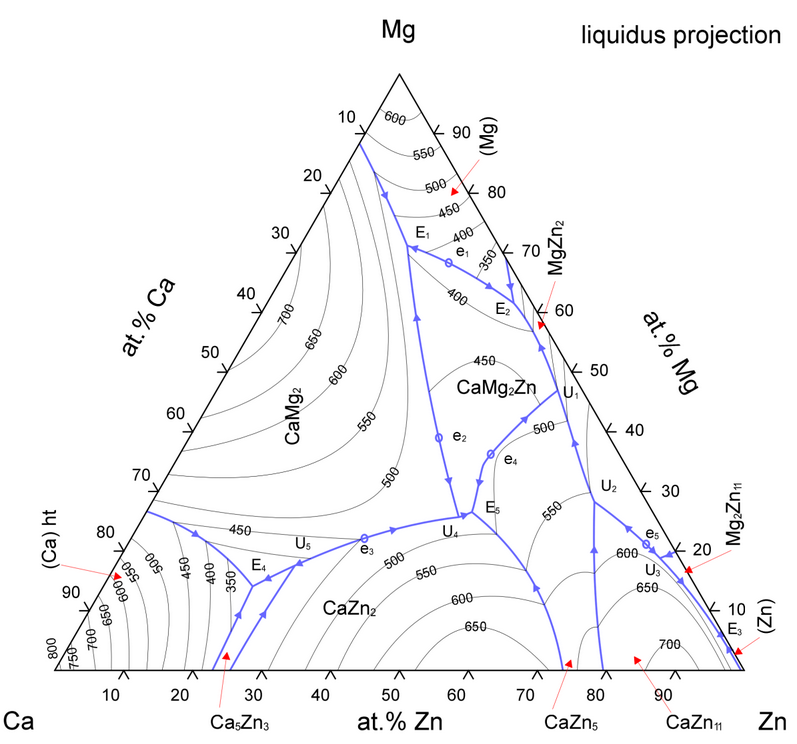
\includegraphics[width=0.9\textwidth]{Ph_MgZnCaLiquidPhase_SprMats.png}
	\caption[Mg-Zn-Ca ternary phase diagram; liquidus projection.]{Mg-Zn-Ca ternary phase diagram; liquidus projection. Reproduced from \cite{Paris1933}}
	\label{fig:MgZnCaLiquidPhaseD}
\end{figure}

%table
\begin{table}[h]
	\centering
	\begin{tabular}{ l l l l l l l l l l }
		\toprule
		Composition & \acrshort{Tg} & \acrshort{Tx} & \acrshort{Tm} & \acrshort{Tl} & \acrshort{dT} & \acrshort{Trg}$_{(m)}$ & \acrshort{Trg}$_{(l)}$ & \acrshort{gfa} & Source \\ 
		& & & & & $(T_{x} - T_{g})$ & $(T_{g}/T_{m})$ & $(T_{g}/T_{l})$ & (mm) & \\ 
		\midrule
		Mg$_{70}$Zn$_{24}$Ca$_{6}$ & 120 & 141 & 352 & 442 & 21 & 0.629 & 0.550 & 3.0 & \cite{Cao2013, Cao2012} \\ 
		Mg$_{68}$Zn$_{26}$Ca$_{6}$ & 128 & 151 & 336 & 406 & 23 & 0.658 & 0.591 & 3.3 & \cite{Cao2013, Cao2012} \\ 
		Mg$_{66}$Zn$_{28}$Ca$_{6}$ & 129 & 155 & 334 & 410 & 26 & 0.662 & 0.589 & 2.8 & \cite{Cao2013, Cao2012} \\ 
		Mg$_{64}$Zn$_{30}$Ca$_{6}$ & 131 & 160 & 335 & 412 & 29 & 0.664 & 0.590 & 2.7 & \cite{Cao2013, Cao2012} \\ 
		Mg$_{62}$Zn$_{32}$Ca$_{6}$ & 138 & 169 & 338 & 424 & 31 & 0.673 & 0.590 & 1.5 & \cite{Cao2013, Cao2012} \\ 
		Mg$_{75}$Zn$_{20}$Ca$_{5}$ & 114 & 122 & 353 & 452.5 & 8 & 0.618 & 0.533 & 1.0 & \cite{Gu2005} \\ 
		Mg$_{70}$Zn$_{25}$Ca$_{5}$ & 124 & 136 & 351 & 398 & 12 & 0.636 & 0.592 & 3.0 & \cite{Gu2005, Zhou2013} \\ 
		Mg$_{67.5}$Zn$_{27.5}$Ca$_{5}$ & 134 & 146 & 336 & 375 & 12 & 0.668 & 0.628 & 4.0 & \cite{Gu2005} \\ 
		Mg$_{68}$Zn$_{28}$Ca$_{5}$ & 134.5 & 145.5 & 333 & 374.5 & 11 & 0.672 & 0.629 & 4.0 & \cite{Gu2005} \\ 
		Mg$_{65}$Zn$_{30}$Ca$_{5}$ & 141.5 & 155 & 336 & 387 & 13.5 & 0.681 & 0.628 & 3.0 & \cite{Gu2005} \\ 
		Mg$_{60}$Zn$_{35}$Ca$_{5}$ & 169 & 174 & 336 & 432.5 & 5 & 0.726 & 0.627 & 2.0 & \cite{Gu2005} \\ 
		Mg$_{72}$Zn$_{24}$Ca$_{4}$ & 84 & 115 & 335 & 420 & 31 & 0.587 & 0.515 & 1.1 & \cite{Cao2013, Cao2012} \\ 
		Mg$_{70}$Zn$_{26}$Ca$_{4}$ & 86 & 126 & 335 & 398 & 40 & 0.590 & 0.535 & 2.8 & \cite{Cao2013, Cao2012} \\ 
		Mg$_{69}$Zn$_{27}$Ca$_{4}$ & 111 & 139 & 339 & 378 & 28 & 0.627 & 0.590 & - & \cite{Wang2013} \\ 
		Mg$_{68}$Zn$_{28}$Ca$_{4}$ & 84 & 135 & 331 & 393 & 51 & 0.591 & 0.536 & 4.0 & \cite{Cao2013, Cao2012} \\ 
		Mg$_{66}$Zn$_{30}$Ca$_{4}$ & 89 & 140 & 336 & 391 & 51 & 0.594 & 0.545 & 3.5 & \cite{Cao2013, Cao2012} \\ 
		Mg$_{64}$Zn$_{32}$Ca$_{4}$ & 89 & 142 & 335 & 436 & 53 & 0.595 & 0.511 & 0.7 & \cite{Cao2013, Cao2012} \\
		\bottomrule 
	\end{tabular}
	\caption[Known basic \acrshort{bmg} properties of several MgZnCa alloys. All temperatures are in \degree C.]{Known basic \acrshort{bmg} properties of several MgZnCa alloys. All temperatures are in \degree C. Temperature values from \cite{Gu2005} have been interpreted from plots, as has \acrshort{Tg} from \cite{Wang2013}. Compiled from \cite{Cao2013, Gu2005, Zhou2013, Cao2012, Wang2013}.}
	\label{tab:MgZnCaAlloys}
\end{table}

%code to put 3 images side by side in a figure
\begin{figure}[htb]
	\centering
	%Image 1
	\begin{subfigure}[htbp]{0.49\textwidth}
		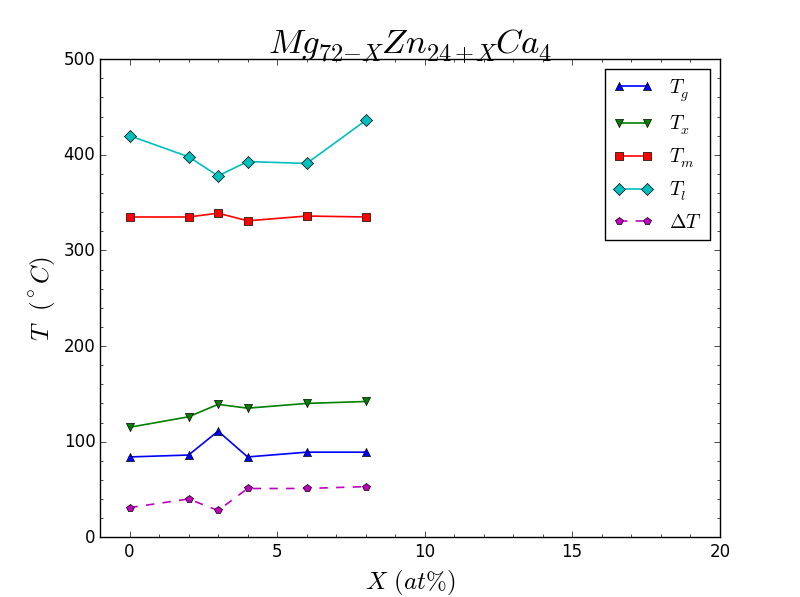
\includegraphics[width=\textwidth]{Mg72-XZn24+XCa4.png}
		\caption{}
		\label{fig:Mg72xZn24xCa4}
	\end{subfigure}
	%Image 2
	\begin{subfigure}[htbp]{0.49\textwidth}
		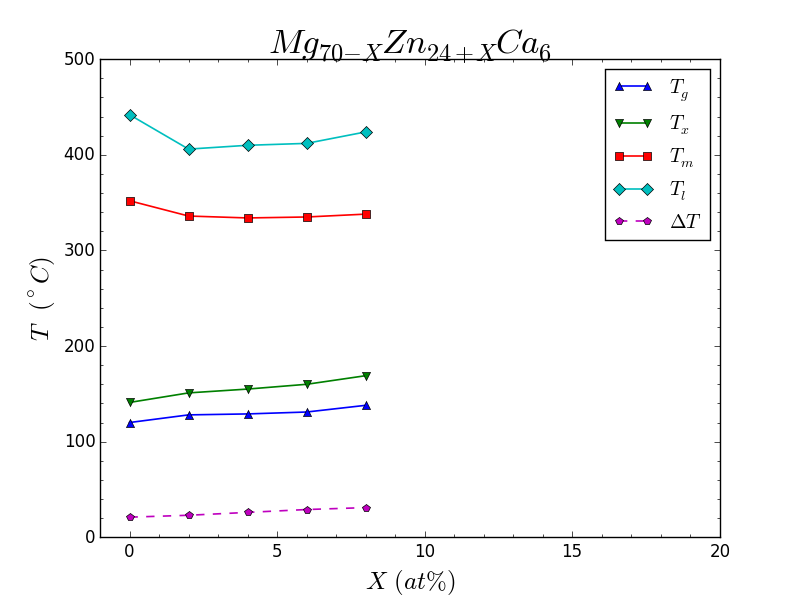
\includegraphics[width=\textwidth]{Mg70-XZn24+XCa6.png}
		\caption{}
		\label{fig:Mg70xZn24xCa6}
	\end{subfigure}
	%Image 3
	\begin{subfigure}[htbp]{0.49\textwidth}
		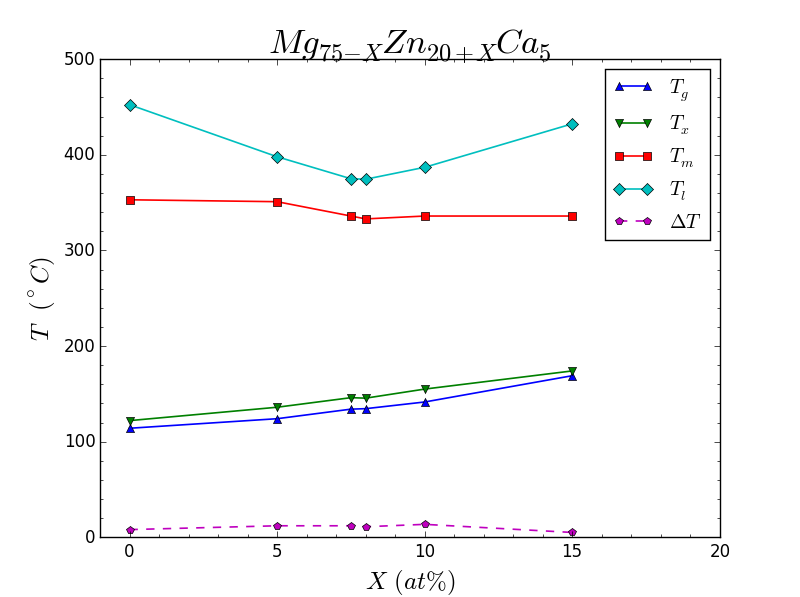
\includegraphics[width=\textwidth]{Mg75-XZn20+XCa5.png}
		\caption{}
		\label{fig:Mg75xZn20xCa5}
	\end{subfigure}
	\caption[Plots of \acrshort{Tg}, \acrshort{Tx}, \acrshort{Tm}, \acrshort{Tl}, and \acrshort{dT} for alloys presented in Table \ref{tab:MgZnCaAlloys}. (a) Mg$_{72-X}$Zn$_{24+X}$Ca$_{4}$, (b) Mg$_{70-X}$Zn$_{24+X}$Ca$_{6}$, (c) Mg$_{75-X}$Zn$_{20+X}$Ca$_{5}$.]{Plots of \acrshort{Tg}, \acrshort{Tx}, \acrshort{Tm}, \acrshort{Tl}, and \acrshort{dT} for alloys presented in Table \ref{tab:MgZnCaAlloys}. (a) Mg$_{72-X}$Zn$_{24+X}$Ca$_{4}$, (b) Mg$_{70-X}$Zn$_{24+X}$Ca$_{6}$, (c) Mg$_{75-X}$Zn$_{20+X}$Ca$_{5}$. Compiled from \cite{Cao2013, Gu2005, Zhou2013, Cao2012, Wang2013}.}%global caption
	\label{fig:MgZnCaPlots}
\end{figure}

\newpage

%%%%%%%%%%%%%%%%%%%%%%%%%%%%%%%%%%%%%%%%%%%%%%%%%%%%%%%%%%%%%%%%%%%%%%%%%%

%Glossary
\printglossaries

\end{document}